\documentclass[10pt,a4paper]{article}

% import en preámbulo
\usepackage[spanish]{babel} % Idioma
\usepackage[utf8]{inputenc} % Codificación
\usepackage{comment} % Permite utilizar el entorno comment
\usepackage{amsmath}
\usepackage{amsthm}
\pagestyle {plain} % Configuración de página
\usepackage{graphicx} % Gráficos
\usepackage{titling}
\usepackage{amsfonts}
%\usepackage{subfigure}
\newcommand{\subtitle}[1]{%
  \posttitle{%
    \par\end{center}
    \begin{center}\large#1\end{center}
    \vskip0.4em}%
}
\usepackage{mathrsfs}
\usepackage[T1]{fontenc}
\usepackage[htt]{hyphenat}
\usepackage{float}
\usepackage{subcaption}
\usepackage[a4paper,top=2cm,bottom=3cm,left=2.5cm,right=2.5cm,marginparwidth=1.75cm]{geometry}
\usepackage{multirow}
\usepackage{siunitx} % For \num and \SI
\sisetup{output-exponent-marker=\ensuremath{\mathrm{e}}}
\usepackage{blindtext}
\usepackage{scrextend}
\usepackage[table]{xcolor}
\usepackage{pdfpages} % Para incluir PDF
%\addtokomafont{labelinglabel}{\sffamily} % For labeling lists
\renewcommand{\labelitemi}{$\bullet$}

\usepackage{hyperref} % Index con hipervinculos :)
\hypersetup{colorlinks,citecolor=black,filecolor=black,linkcolor=black,urlcolor=black}
%\captionsetup[figure]{labelfont={bf},name={Figura},labelsep=period}
%\captionsetup[table]{labelfont={bf},name={Tabla},labelsep=period}
\renewcommand{\spanishtablename}{Tabla}

\usepackage{etoolbox}
\makeatletter
\patchcmd{\@makecaption}
  {\scshape}
  {}
  {}
  {}
\makeatother


\usepackage{cancel}

\usepackage{empheq}

%\usepackage{minipage}

\newtheorem{mydef}{Definición}

%Directorio de imágenes
\graphicspath{{./img/}}

%Para bibliografía
\usepackage[backend=bibtex,style=numeric,sorting=none]{biblatex}
\addbibresource{bib_file.bib}

\usepackage{csquotes}

\DeclareRobustCommand*{\ora}{\overrightarrow}

% Comienzo del documento
\begin{document}

\newcommand{\HRule}{\rule{\linewidth}{0.5mm}}
\begin{center}
{\LARGE Tesis de Ingeniería Electrónica}\\[0.5cm]
\textbf{\Large Diseño y Construcción de una Computadora de Vuelo para Vehículos Autónomos con Tolerancia a Fallas}\\[0.6cm]
\end{center}

\begin{center}
        \begin{tabular}{lllll}
                Alumno: & & & & \\
                        & 98211 & Nuñez Frau Federico Ignacio & fnunezf@fi.uba.ar & %1130888185
                        \\
                & & & & \\
                Director: & & & & \\
                & 203004 & Pose Claudio & cldpose@fi.uba.ar & %1166889316
                \\ 
                & & & & \\
                Co-director: & & & & \\
                & %{\color{red} COMPLETAR} 
                & Garberoglio Leonardo & lgarberoglio@frsn.utn.edu.ar & %{\color{red} COMPLETAR}
                \\ 
        \end{tabular}
\end{center}

\vspace{0.3cm}

\begin{center}
        %{\color{red} COMPLETAR LA FECHA}
        25 de septiembre de 2023
\end{center}

\vspace{1.0cm}
\tableofcontents
\newpage

\section{Objetivo}

%Objetivo: a dónde querés llegar con este trabajo. Acá describo en 1 ó 2 páginas cuál es el objetivo, es decir: 
%- El análisis de las características de sistemas críticos en general. 
%- La construcción de la placa para usar como computadora de vuelo.
%- El desarrollo del prototipo, simulando las fallas.

El presente trabajo de tesis tiene por objetivo el diseño y construcción de una computadora de vuelo de bajo nivel, a ser utilizada en un vehículo aéreo hexarotor, no tripulado. Como aspecto particular, esta debe contar con la capacidad de tolerar fallas %de hardware y de software 
que puedan ocurrir en pleno vuelo. Lo que se busca es que estas fallas no impacten en la misión del vehículo y que puedan ser detectadas lo antes posible para tomar una acción.

En primera medida, se hace un análisis e investigación acerca del estado del arte, para vehículos aéreos no tripulados de caracter comercial. El objetivo es conocer los mecanismos de seguridad que comúnmente se aplican en este tipo de vehículos.%, tanto de hardware como de software. Por otro lado, se busca conocer cuáles son las normas actuales pertinentes al uso y comercialización de este tipo de vehículos.

En cuanto al desarrollo de la computadora de vuelo, esto comprende la definición de los requerimientos de la misma, principalmente de hardware en cuanto a sensores, conectores y funcionalidades deseadas. Se realiza una investigación de la variedad de componentes disponibles, para luego pasar a una etapa de selección de los componentes a utilizar. Por último, se define un circuito esquemático y se diseña un PCB, el cual será enviado a fabricación.

%Para abordar la tolerancia a fallas de la computadora de vuelo, se plantea utilizar técnicas que involucran la redundancia, tanto de hardware como de software. Para ello, se lleva a cabo una investigación de las técnicas comúnmente utilizadas en el sector aeronáutico para tolerancia de fallas. Finalmente, se define un esquema y una arquitectura a utilizar como mecanismo de tolerancia a fallas.

%Para demostrar los resultados, se presentan resultados de pruebas de control de un motor en una arquitectura redundante, sobre la cual se simula la manifestación de distintos tipos de fallas. Se presentan los resultados y la respuesta del sistema.

Para demostrar el funcionamiento de la computadora de vuelo, se presentan resultados donde se emulan distintas fallas sobre uno de los sensores, la unidad de medición inercial (IMU). Se presentan los resultados y el comportamiento del sistema frente a estas fallas.

\section{Introducción}\label{sec:Introduccion}

%Introducción: acá se pone en contexto, por ejemplo se puede describir el proyecto del LAR y llegar a que uno de los elementos del drone es la computadora de vuelo, pertinente a este trabajo. También acá, tendría que mencionar el por qué de la tolerancia a fallas. Podría dar algún ejemplo de algún accidente que haya ocurrido. Por último, ejemplos de usos y aplicaciones civiles. Acá se justifica el por qué de la tolerancia a fallas. En las siguientes secciones se explica cómo se aborda y qué se desarrolló.

Los vehículos aéreos no tripulados (UAVs) originalmente fueron desarrollados para uso en aplicaciones militares. Al no contar con un piloto ni con una tripulación a bordo, estos permiten llevar adelante tareas peligrosas, que pueden llegar a poner en riesgo la vida de las personas. Sumado a esto, el desarrollo y mantenimiento de este tipo de vehículos resulta menos costoso frente al de un avión tripulado \cite[p.~490]{collinson2023introduction}. Estos factores fueron claves como motivación para el desarrollo de este tipo de vehículos.

Algunos de los principales usos en el ámbito militar son reconocimiento, vigilancia y monitoreo. Al contar con distintos tipos de sensores, como cámaras, sensores infrarrojos, entre otros, estos pueden recolectar información en zonas hostiles, de manera económica y segura.

A partir de los avances en la tecnología y la reducción en los costos de fabricación, tanto para sensores como componentes en general, este tipo de vehículos han comenzado a ser utilizados para fines civiles y comerciales. De esta manera, las mismas ventajas por las cuales comenzaron a ser utilizados en el ámbito militar, despertaron el interés de distintos sectores por fuera de este. Hoy en día estos vehículos son utilizados para distintas aplicaciones civiles y comerciales. Algunas de ellas son:

\begin{itemize}
    \item Búsqueda y Rescate: En escenarios de desastres naturales, los UAVs son utilizados para tomar imágenes y videos de las zonas afectadas o búsqueda de personas. El uso de un UAV frente a un avión o helicóptero, elimina potenciales riesgos para el piloto y la tripulación, además de reducir el costo de la operación. Un ejemplo relevante de este uso de UAVs fue durante el accidente nuclear de Fukushima del año 2011 ocurrido en Japón. Debido a la radiación de la zona, el uso de UAVs fue necesario para la recolección de imágenes y video. Además, se utilizó un UAV de la Fuerza Aérea de Estados Unidos (FAA) equipado con un sensor infrarrojo para conocer la temperatura de los reactores nucleares \cite{adams2011survey}.
    \item Teledetección: El bajo coste de los UAVs permite obtener gran cantidad de datos para distintas investigaciones del suelo y del medio ambiente. En \cite{villa2016overview} se puede encontrar un trabajo en donde se utilizaron vehículos aéreos no tripulados para realizar un muestreo ambiental en el Ártico, además de estudios acerca de la temperatura de la superficie del océano. En \cite{mcgonigle2008unmanned} se presenta un trabajo donde se utiliza un UAV para realizar mediciones sobre gases volcánicos. Utilizando distintos tipos de espectrómetros y sensores electroquímicos, se analizan las concentraciones de dióxido de carbono y dióxido de azufre.
    \item Inspección en Infraestructura y Construcciones: Utilizando UAVs es posible realizar tareas de inspección para encontrar problemas en la red de distribución de energía eléctrica \cite{luque2014power}. Existen algunas empresas que se dedican a estas actividades de inspección, como por ejemplo Cyberhawk. Esta además ofrece otros servicios destinados a distintos sectores industriales, como monitoreo en construcciones y de generadores eólicos.
    \item Agricultura de Precisión: El uso de UAVs en este sector está destinado a mejorar el rendimiento del cultivo, a través de distintas actividades como el riego programado, la detección temprana de pestes y el sensado de la textura del suelo. Este último puede usarse como indicador de la calidad del suelo para cultivo.
    \item Vigilancia: Los UAVs se utilizan para patrullar y controlar las fronteras, por ejemplo para detectar situaciones de tráfico ilegal.
\end{itemize}

El factor común a todas estas aplicaciones es que la incorporación de los UAVs en el ámbito civil y comercial ha abierto oportunidades para realizar tareas y actividades que de otra forma serían muy costosas y/o riesgosas para las personas.

Teniendo en cuenta la importancia que han tomado, además del hecho de que en muchas de estas aplicaciones estos sobrevuelan zonas donde circulan personas, resulta mandatorio garantizar cierto grado de confiabilidad en su funcionamiento. Este es un aspecto que caracteriza la capacidad de un sistema para funcionar correctamente durante un período de tiempo, donde ``correctamente'' se refiere a cumplir con la tarea para el cual fue diseñado. Para el caso de un UAV, el hecho de volar en espacio aéreo civil puede llegar a causar daño físico a personas, si es que un vehículo presenta una falla y por ejemplo pierde el control. Otra de las posibles consecuencias tiene que ver con los costos que puede ocasionar una falla en una misión relacionada a una actividad laboral. El hecho de tener que repetir la misión puede traer mayores costos para la actividad en cuestión.

Un UAV típicamente se compone de distintos elementos. Cada uno de ellos es susceptible de manifestar distintos tipos de fallas que pueden afectar al vehículo de distintas maneras. Algunos de los elementos más importantes son la estructura mecánica, el sistema de batería y alimentación, los motores y actuadores, un sistema de comunicación remota con un piloto y la computadora de vuelo. En este trabajo se abordarán aspectos relacionados a fallas relacionadas con este último.

\subsection{Computadora de Vuelo}

La computadora de vuelo se compone de una unidad de procesamiento que realiza la adquisición de datos de sensores y ejecuta los algoritmos necesarios para estabilizar y controlar el vehículo. Suelen incorporar una variedad de sensores a bordo, siendo el más común de ellos la Unidad de Medición Inercial (IMU), compuesta por acelerómetros y giróscopos triaxiales. A su vez, suelen disponer de magnetómetros triaxiales, barómetros, GPS, LiDARs, sensores ultrasónicos, sensores de flujo óptico, entre otros diferentes tipos de sensores de velocidad y distancia. Sumado a esto, suelen contar con distintas interfaces para comunicación con otros módulos externos, como pueden ser sensores, actuadores u otros que sean de uso específico para cumplir con la misión del vehículo.

Los datos de los sensores son utilizados para ejecutar los distintos algoritmos de navegación y control. Periódicamente se adquieren mediciones de los distintos sensores del vehículo, se procesan dichos datos para luego aplicar acciones de control a los distintos actuadores, es decir actuar sobre los motores. De esta manera se logra que el vehículo recorra una trayectoria previamente configurada, o bien que responda adecuadamente a los comandos enviados por un piloto a distancia.

%Se encarga de adquirir datos de los sensores, ejecutar los algoritmos necesarios para estabilizar y controlar el vehículo y aplicar los resultados a sus actuadores, es decir sobre los motores del vehículo.


%Para ello, periódicamente se adquieren mediciones de los distintos sensores del vehículo, se procesan dichos datos para luego aplicar acciones de control a los distintos actuadores, es decir actuar sobre los motores. De esta manera se logra que el vehículo recorra una trayectoria previamente configurada, o bien que responda adecuadamente a los comandos enviados por un piloto a distancia.


%La computadora de vuelo es el elemento central en un vehículo aéreo no tripulado. Esta centraliza toda la información. Se encarga de realizar la adquisición de datos de sensores y ejecutar los algoritmos necesarios para estabilizar y controlar el vehículo. Para ello, periódicamente se adquieren mediciones de los distintos sensores del vehículo, se procesan dichos datos para luego aplicar acciones de control a los distintos actuadores, es decir actuar sobre los motores. De esta manera se logra que el vehículo recorra una trayectoria previamente configurada, o bien que responda adecuadamente a los comandos enviados por un piloto a distancia.

%\subsection{Características de la Computadora de Vuelo a Desarrollar}
%\subsection{Características y Objetivos Particulares}
\subsection{Tolerancia a Fallas y Redundancias}

Resulta evidente que la computadora de vuelo es el elemento central en un vehículo aéreo no tripulado, por lo que una falla puede traer consecuencias graves. Por ejemplo, una falla en una lectura de un sensor, puede resultar en una mala estimación de la posición del vehículo o incluso decantar en la pérdida de control de este. En vehículos aéreos tripulados como aviones comerciales y militares, es común que se utilicen distintas técnicas de tolerancia a fallas para mejorar la confiabilidad. Esto mismo ocurre con vehículos aéreos no tripulados de uso militar, aunque no es tan común en aquellos de uso civil y comercial. 

La computadora de vuelo de este trabajo se desarrollará teniendo como objetivo la necesidad de implementar técnicas de tolerancia a fallas a partir del uso de redundancias. Esta es la principal técnica utilizada en sistemas de tiempo real \cite{nelson1990fault} e implica que las tareas realizadas se ejecuten utilizando réplicas de hardware. En el eventual caso de que una de estas réplicas presente una falla y el sistema la detecte, luego se puede tomar una acción, como por ejemplo descartar la réplica fallada y utilizar alguna de las réplicas sin fallas. 

El solo hecho de incoporar redundancias en un sistema no equivale a incrementar la confiabilidad. Es necesario incorporar mecanismos que administren correctamente los aspectos relacionados al manejo de las redundancias. La forma más común de detectar fallas es realizando comparaciones entre los resultados calculados por cada réplica. Por ejemplo, si se contara con un sistema con doble redundancia, podría concluirse que alguna de las dos réplicas presentó una falla a partir de la comparación de los resultados obtenidos por cada réplica. Sin embargo, a priori no podría decirse cuál de estas fue la que falló. Ambas réplicas deberían ejecutar una rutina auxiliar que realice una verificación interna. Teniendo en cuenta que el sistema de control de vuelo del UAV es un sistema de tiempo real, la ejecución de esta rutina podría perjudicar su determinismo temporal y poner en riesgo la estabilidad del vehículo. Este ejemplo ilustra la necesidad de analizar y administrar correctamente los aspectos relacionados al manejo de las redundancias.

En es te trabajo se diseñará el circuito correspondiente a la computadora de vuelo y se fabricarán tres réplicas, cada una en su propio PCB. Luego de verificar el correcto funcionamiento de cada una de estas por separado, se procederá a proponer una arquitectura distribuida, para administrar las redundancias. Finalmente, se utilizarán las tres placas para demostrar el funcionamiento del sistema redundante.

%A partir de la comparación de los resultados obtenidos por cada réplica, es posible detectar fallas y tomar acciones que permitan continuar con la misión del vehículo.

%Se toman las consideraciones necesarias para la conexión y gestión de la información entre las tres réplicas. Se plantea una arquitectura distribuida, donde cada nodo recibe los datos adquiridos por las demás y ejecuta un algoritmo para corroborar la consistencia de los mismos. Para validar el funcionamiento, se realiza una prueba experimental donde se detecta la falla de una unidad inercial.

%En este contexto, el objetivo de este trabajo de Tesis es el diseño y construcción de una computadora de vuelo, con la capacidad de implementar mecanismos de tolerancia a fallas, a partir de redundancias, utilizando componentes commercial off-the-shelf (COTS).

%En este contexto, el objetivo de este trabajo de Tesis es el diseño y construcción de una computadora de vuelo, con la capacidad de implementar mecanismos de tolerancia a fallas, a partir de redundancias, utilizando componentes commercial off-the-shelf (COTS).

%Un UAV típicamente se compone de varios elementos, como una estructura mecánica, un sistema de batería y alimentación para el vehículo, sus motores y actuadores, un sistema de comunicación remota con un piloto y una computadora de vuelo. Si bien cada uno de estos es susceptible de manifestar distintos tipos de fallas que puedan afectar al vehículo de distintas formas, en este trabajo se abordarán aspectos relacionados a fallas en la computadora de vuelo. Este es el elemento central...

%En los últimos años se ha incrementado mucho la presencia de UAVs en espacio aéreo civil. Debido a esto, se plantea que los UAVs deberían presentar características que permitan un funcionamiento correcto, tolerante a fallas. Como consecuencias posibles, el hecho de volar en espacio aéreo civil puede llegar a causar daño físico a personas, si es que un vehículo presenta una falla y por ejemplo pierde el control. Otra de las posibles consecuencias tiene que ver con los costos que puede ocasionar una falla en una misión relacionada a una actividad laboral. El hecho de tener que repetir la misión puede traer mayores costos para la actividad en cuestión. El objetivo del diseño tolerante a fallas consiste en mejorar la confianza (Dependability) del sistema, apuntando a que este pueda seguir ejecutando su función de manera correcta a pesar de la presencia de una cierta cantidad de fallas [54]. De esta última expresión se puede tomar una definición de lo que es un sistema tolerante a fallas

%En vehículos aéreos tripulados como aviones comerciales y militares, es común que para ello se utilicen técnicas de tolerancia a fallas a partir de redundancias. Esto mismo ocurre con vehículos aéreos no tripulados de uso militar, aunque no es tan común en aquellos de uso civil y comercial. En este contexto, el objetivo de este trabajo de Tesis es el diseño y construcción de una computadora de vuelo, con la capacidad de implementar mecanismos de tolerancia a fallas, a partir de redundancias, utilizando componentes commercial off-the-shelf (COTS).

%En los últimos años ha habido un incremento en el uso de vehículos aéreos no tripulados... Esto implica que se requiere cierto grado de confiabilidad...\\

%La computadora de vuelo se compone de ...\\

%Un sistema crítico (en inglés \textit{safety-critical system}) es aquel en el que un fracaso puede traer consigo consecuencias catastróficas, como daños graves a personas, pérdida de vidas o daños importantes al medio ambiente \cite[p.~271]{kopetz-2011}. Por su definición, un sistema puede caracterízarse como crítico o no crítico antes de su implementación, ya que lo que determina esto es simplemente el uso que se le dará. Algunas áreas típicas donde se pueden encontrar estos sistemas son aviónica, equipamiento médico y energía nuclear.\\

%\textbf{{\color{red} COMPLETAR}}

%\section{Análisis de Sistemas Críticos y Tolerancia a Fallas}

\section{Estado del Arte}\label{sec:estado_del_arte}

En esta sección se analizan distintos casos de implementación de sistemas de control de vuelo redundantes. Si bien en este trabajo se desarrolla una computadora de vuelo para UAVs, se toma como referencia características generales del funcionamiento del sistema utilizado en aviones comerciales, por ser el sistema críticos por excelencia. Estos funcionan correctamente durante muchas horas, trasladando a muchas personas. Seguido a esto, se analizan trabajos y computadoras de vuelo utilizadas en UAVs que implementen redundancias. Los sismteas analizados utilizan distintas técnicas para implenetar las redundancias. Lo que se busca es detectar similitudes y posibles requerimientos que caractericen a un sistema con redundancias. 

\subsection{Redundancias en Sistemas de Control de Vuelo en Aviones}

En aviónica, el sistema de control de vuelo es sin dudas un sistema crítico. Originalmente constituidos por sistemas mecánicos complejos, estos fueron reemplazados por sistemas denominados \textit{fly-by-wire}, introducidos en vuelos comerciales en el Airbus 320 en 1987 y el Boeing 777 en 1994 \cite{FBWNASA}, con el objetivo de alivianar la carga del avión y mejorar su rendimiento en cuanto al consumo de combustible. Su nombre deriva del hecho de que la acción de control del piloto no es directa sobre el avión, sino que es una computadora la que la ejecuta. Todas las señales de sensores y de comandos son transmitidas eléctricamente desde y hacia una computadora de vuelo.\\

A modo de ejemplo en la figura \ref{fig:Boeing_777_diagrama}, se muestra un diagrama simplificado de la arquitectura del sistema de control de vuelo principal del avión Boeing 777. En esta imagen se muestran distintos bloques los cuales se encuentran comunicados a través de un bus. Cuando el piloto del avión quiere ejecutar una acción, este lo hace a través de métodos convencionales como palancas o pedales que se encuentran en la cabina. Estas acciones generan señales analógicas las cuales son entregadas a los bloques denominados \textit{Actuator Control Electronics} (ACEs). Estos bloques convierten la señal analógica en una señal digital que puede enviarse a través del bus de comunicaciones a los bloques denominados \textit{Primary Flight Control System} (PFCs).

\begin{figure}[H]
    \centering
    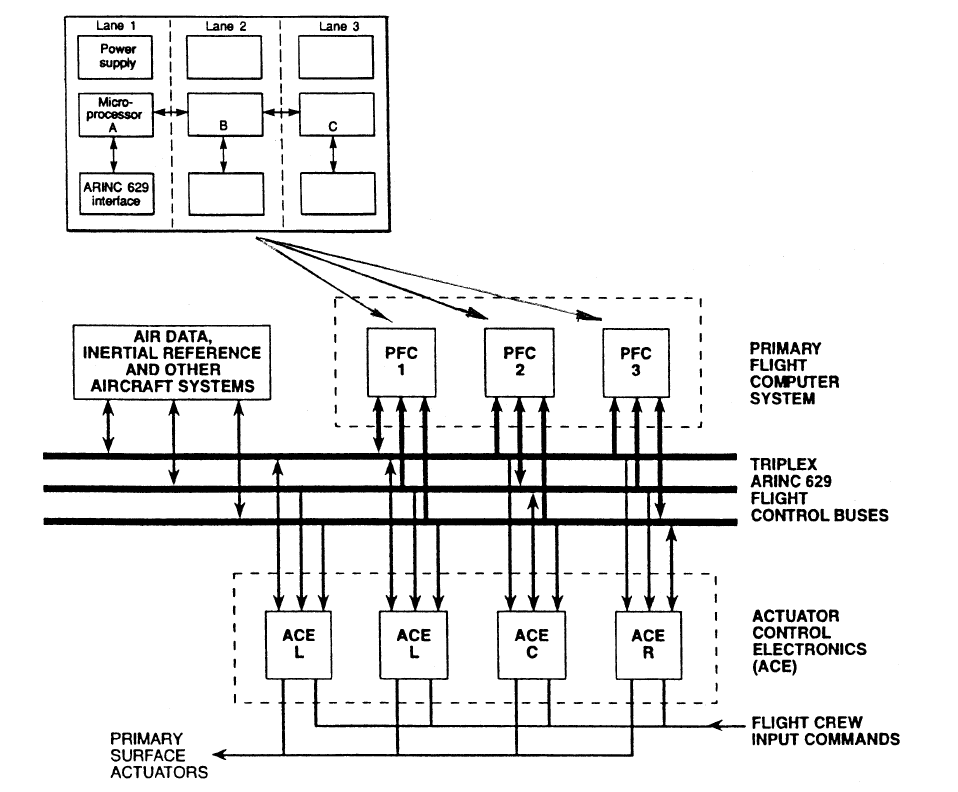
\includegraphics[width=0.7\textwidth]{img/Boeing_777_diagrama.png}
    \caption{Arquitectura del sistema principal de vuelo, conformado por varias computadoras en una configuración redundante. La imagen se extrajo de \cite{collinson2023introduction}.}
    \label{fig:Boeing_777_diagrama}
\end{figure}

Además de la acción del piloto, las PFCs toman datos de los distintos sensores para poder calcular todas las acciones de control que se aplicarán a los distintos actuadores del avión. Los resultados de los cálculos son enviados a los actuadores nuevamente a través del bus de comunicación a cada bloque ACE asignado para cada actuador el cual interpreta el comando recibido por el bus y lo convierte en una señal analógica que aplicará su actuador asignado. En \cite{yeh1996triple} puede encontrarse una explicación más detallada del funcionamiento de este sistema en el avión Boeing 777.\\

En la figura \ref{fig:Boeing_777_diagrama} lo que se observa es que hay redundancias en los bloques PFCs y ACEs. No solo eso, sino que además hay redundancias en el canal de comunicación, es decir en el bus. Por si fuera poco, en el Boeing 777, cada una de las PFCs se compone a su vez de 3 microprocesadores, cada uno con su fuente de alimentación propia e interfaz de comunicación con el bus. Cada uno de esos 3 procesadores son de distintos fabricantes y sus respectivos softwares son desarrollados por grupos de trabajo distintos. Generalmente solo un procesador de cada PFC se encuentra en funcionamiento normal y los otros actúan como monitores, verificando que lo que estas calculan es correcto.\\

Sin dudas todo el sistema de control de vuelo presenta una complejidad muy grande. El hecho de incorporar redundancias en el sistema incrementa notablemente la seguridad. La forma en la que esta se cuantifica es a través de la probabilidad de que el sistema fracase de forma catastrófica. Para aviones comerciales típicamente debe ser $10^{-9}/h$ \cite[p.~217]{collinson2023introduction}. Este valor es tan bajo que incluso es imposible de verificar de forma expermiental, ya que habría que ejecutar el sistema durante $10^9$ horas aproximadamente. La probabilidad de falla de los semiconductores no alcanza este valor \cite[p.~272]{kopetz-2011}. Este es el motivo por el cual se incluyen bloques redundantes en los sistemas de control de vuelo. Por ejemplo, el hecho de que cada PFC tenga 3 procesadores de distintos fabricantes permite eliminar problemas que sean propios del componente. A su vez, el hecho de que cada procesador tenga un software distinto desarrollado por un grupo de personas distinto permite que las fallas que estos puedan tener sean eliminadas a tiempo.\\

{\color{red} ACÁ AGREGAR UNA CUENTA SÚPER FÁCIL CON UN SISTEMA CON REDUDANCIAS EN PARALELO Y CON LA PROBABILIDAD DE FALLA EXPONENCIAL}.

El uso de redundancias trae consigo la necesidad de un sistema que administre todas las tareas de manera correcta con el objetivo de cumplir con el nivel de seguridad requerido. Por ejemplo, en el caso del Boeing 777 antes mencionado, detectar cuándo una de las PFCs llegó a un cálculo de la ley de control incorrecto, determinar si un sensor del avión dejó de funcionar y qué acción tomar en cada caso, entre otras.\\

En la figura \ref{fig:diagrama_general_fly_by_wire} se muestra un diagrama que representa de forma general la comunicación entre los distintos elementos del sistema de control de vuelo. En este se puede ver la redundancia de buses, sensores, actudaores y computadoras de vuelo.

\begin{figure}[H]
    \centering
    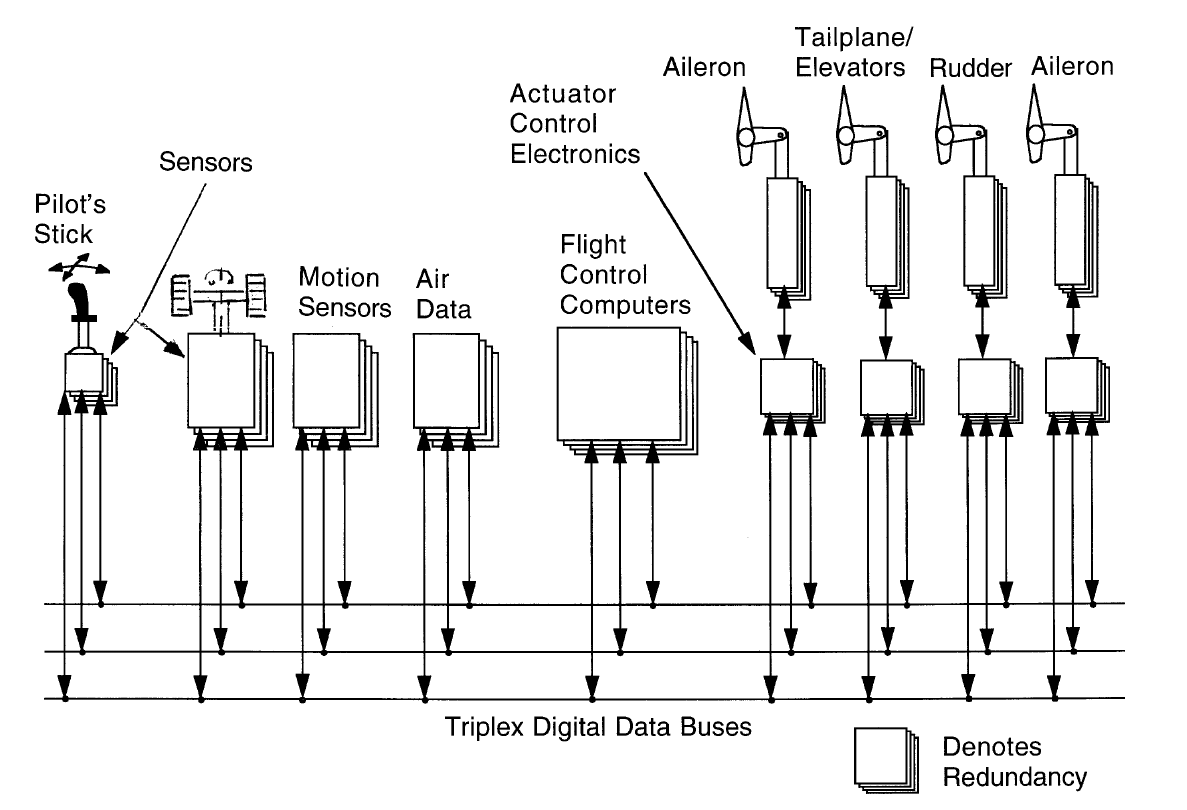
\includegraphics[width=0.8\textwidth]{img/diagrama_general_fly_by_wire.png}
    \caption{Se muestra de manera general las conexiones entre los distintos elementos del sistema de control de vuelo típico en aviones. La imagen se extrajo de \cite{collinson2023introduction}.}
    \label{fig:diagrama_general_fly_by_wire}    
\end{figure}

Cada uno de estos elementos conforman el sistema de control de vuelo tolerante a fallas en aviones. A continuación se analizan algunas de sus características.

\subsubsection{Bus de Comunicaciones}

Hasta principios de los años 70s, la comunicación entre los distintos módulos dentro de los aviones se realizaba a través de arneses de muchos cables que transmitían información en paralelo. Estos eran tan grandes que podían llegar a pesar cientos de kilogramos. Sumado a esto, la enorme cantidad de cables venía acompañada de muchas conexiones, puntos que son típicos causales de fallas intermitentes. A partir de mediados de los años 70s, se comenzó a implementar el uso de buses de comunicación serial, comunes a todos los módulos del avión. Esto simplificó muchísimo el cableado, además de facilitar el desarrollo de módulos de aviónica, ya que se simplificó la forma de comunicación con el resto del avión.\\

La comunicación serial a través del bus utiliza un acceso al medio compartido dominado por el tiempo, \textit{time-division multiple acces} (TDMA). Siguiendo con el caso del avión Boeing 777, el protocolo utilizado es el ARINC 629. Este funciona sin un nodo master y permite una conexión de hasta 120 nodos. Solamente uno de ellos puede acceder al medio físico a la vez, lo cual se define por el acceso al medio dominado por el tiempo. El medio de transmisión es un par trenzado, con una velocidad de 2 Mbit/s. A continuación, en la figura \ref{fig:ARINC_629_bus} se muestra el bus ARINC 629.

\begin{figure}[H]
    \centering
    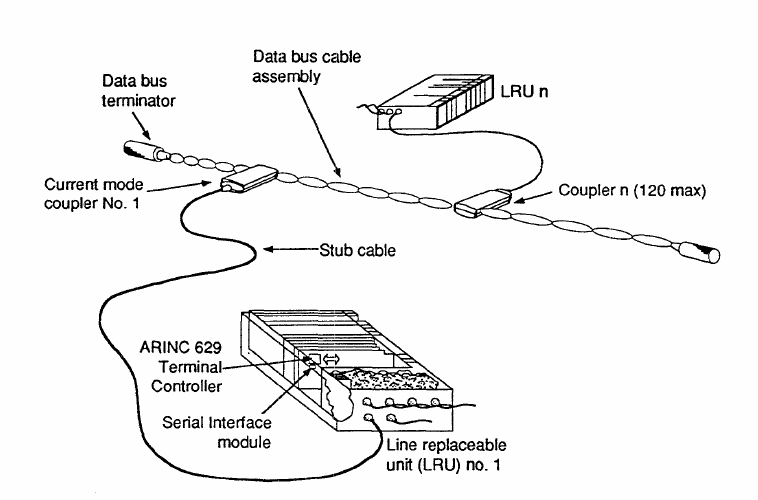
\includegraphics[width=0.7\textwidth]{img/ARINC_629_bus.png}
    \caption{Se muestra un bus ARINC 629 con 2 nodos conectados. Este consiste en un par trenzado, con terminaciones en los extremos para evitar reflexiones. La conexión de los nodos al bus no es directa si no que se utilizan acopladores. La imagen se extrajo de \cite{yeh1996triple}.}
    \label{fig:ARINC_629_bus}    
\end{figure}

El hecho de que todas las comunicaciones pasen por el mismo bus lo vuelve un punto clave en cuanto a la seguridad, ya que una falla en uno de sus cables dejaría a todos los módulos sin comunicación. Es por esto que se incluyen varios buses de estos en paralelo, como se mostró en la figura \ref{fig:diagrama_general_fly_by_wire}.\\

Un aspecto a destacar en el bus de comunicaciones es el método de acceso al medio utilizado, TDMA. El envío y recepción de mensajes se implementa por turnos. Este protocolo define en qué instantes de tiempo cada uno de los nodos puede utilizar el medio físico y en cuáles no. Para que no haya colisiones, todos los nodos deben respetar ese timing, el cual se encuentra predefinido. Esto le da determinismo y claridad al comportamiento del bus y del sistema, ya que a priori puede saberse qué mensaje se estará enviando en cada instante de tiempo. Cualquier otro tipo de comportamiento respresentará una falla. Además, al tratarse de un sistema de tiempo real, no pueden permitirse las retransmisiones, ya que es evidente que se rompería el requerimiento intrínseco de este tipo de sistemas, que es cumplir con la tarea asignada antes de cierto tiempo.

\subsubsection{Comparación de Resultados y Tolerancia a Fallas}

El mecanismo de tolerancia a fallas es a través de la comparación entre mediciones de sensores y resultados de cálculo de la ley de control. Si todos los sensores redundantes funcionan adecuadamente, es esperable que estos entreguen mediciones muy similares. Por otro lado, si uno de ellos entrega una medición diferente a la de los otros dos, se asume que este presentó una medición incorrecta. Como resultado de la comparación, se obtiene un único valor el cual es utilizado por el sistema de control. De la misma forma, se realiza una comparación de los resultados del cálculo de la ley de control obtenido por cada una de las computadoras. Una vez que se decide por un único valor, se envía la señal de actuación.\\

Existen muchos criterios utilizados para seleccionar los valores de sensores. Un aspecto importante a tener en cuenta es que a pesar de que todos los sensores redundantes funcionen adecuadamente, estos presentarán ciertas diferencias en las mediciones, algo que es esperable teniendo en cuenta cuestiones propias de la construcción de cada sensor, ruido, etc. Esto debe ser tenido en cuenta al momento de realizar las comparaciones.\\

En \cite[p.~221]{collinson2023introduction} se menciona un algoritmo muy simple. Este consiste en tomar una de las mediciones como referencia y comparar las demás contra esta. En la figura \ref{fig:votacion_sensores} se toma el ángulo $\theta_1$ como referencia, ya que $\theta_3 > \theta_1 > \theta_2$. En caso de que la diferencia $| \theta_1 - \theta_2 |$ ó $| \theta_1 - \theta_3 |$ supere un cierto límite, se asume que el sensor presentó una falla. En el caso de la imagen, la diferencia con el sensor 2 es mucho mayor que con el 3 y se asume que este presentó una falla. El valor que se toma como válido es el valor intermedio, $\theta_1$.

\begin{figure}[H]
    \centering
    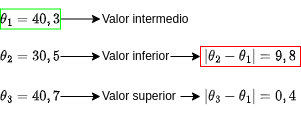
\includegraphics[width=0.5\textwidth]{img/votacion_sensores.png}
    \caption{La comparación entre 3 sensores da como resultado que el sensor 2 presentó una falla. En consecuencia deberá tomarse una acción, por ejemplo ignorar al sensor en próximas mediciones o informar al piloto.}
    \label{fig:votacion_sensores}
\end{figure}

Este mismo esquema se repite luego del cálculo de la ley de control y de los valores a aplicar sobre cada actuador.

\subsection{Redundancias en Sistemas de Control de Vuelo en UAVs}

Es evidente que las consecuencias del fracaso del sistema de control de vuelo en un vehículo aéreo no tripulado, no son las mismas que en un avión comercial. Estos últimos pueden trasladar cientos de personas y realizar vuelos de muchas horas, mientras que en los primeros no hay tripulación ni piloto a bordo del vehículo. Debido a esto, suelen estar construidos con otros requerimientos de seguridad más laxos. Para UAVs de uso militar, la probabilidad de fracaso se encuentra en el orden de $10^{-5} / h$ \cite{zhang2020architecture}\cite[p.~491]{collinson2023introduction}, una diferencia de varios órdenes de magnitud respecto de los aviones comerciales.\\

Al igual que en aviones de uso comercial y militar, es común el uso de redundancias en UAVs de uso militar. {\color{red} CITAR VARIOS EJEMPLOS}.\\

En el caso de UAVs de uso civil y comercial, el uso de redundancias no es tan común. Sin embargo, existen algunas empresas que comercializan computadoras de vuelo con capacidad de utilizar redundancias. A continuación se mencionan algunas de ellas.\\

\subsubsection{Computadoras de Vuelo Comerciales}

La empresa Embention comercializa una computadora de vuelo con redundancia triple, con la posibilidad de incorporar una cuarta computadora extra \cite{embention-2023}. Su funcionamiento se basa en que todas las computadoras de vuelo redundantes se comunican con un elemento denominado árbitro. Este ejecuta un algoritmo de votación y selecciona cuál de las tres computadoras de vuelo es la correcta. En la figura \ref{fig:Veronte_Embention} se muestra un diagrama en bloques.

\begin{figure}[H]
    \centering
    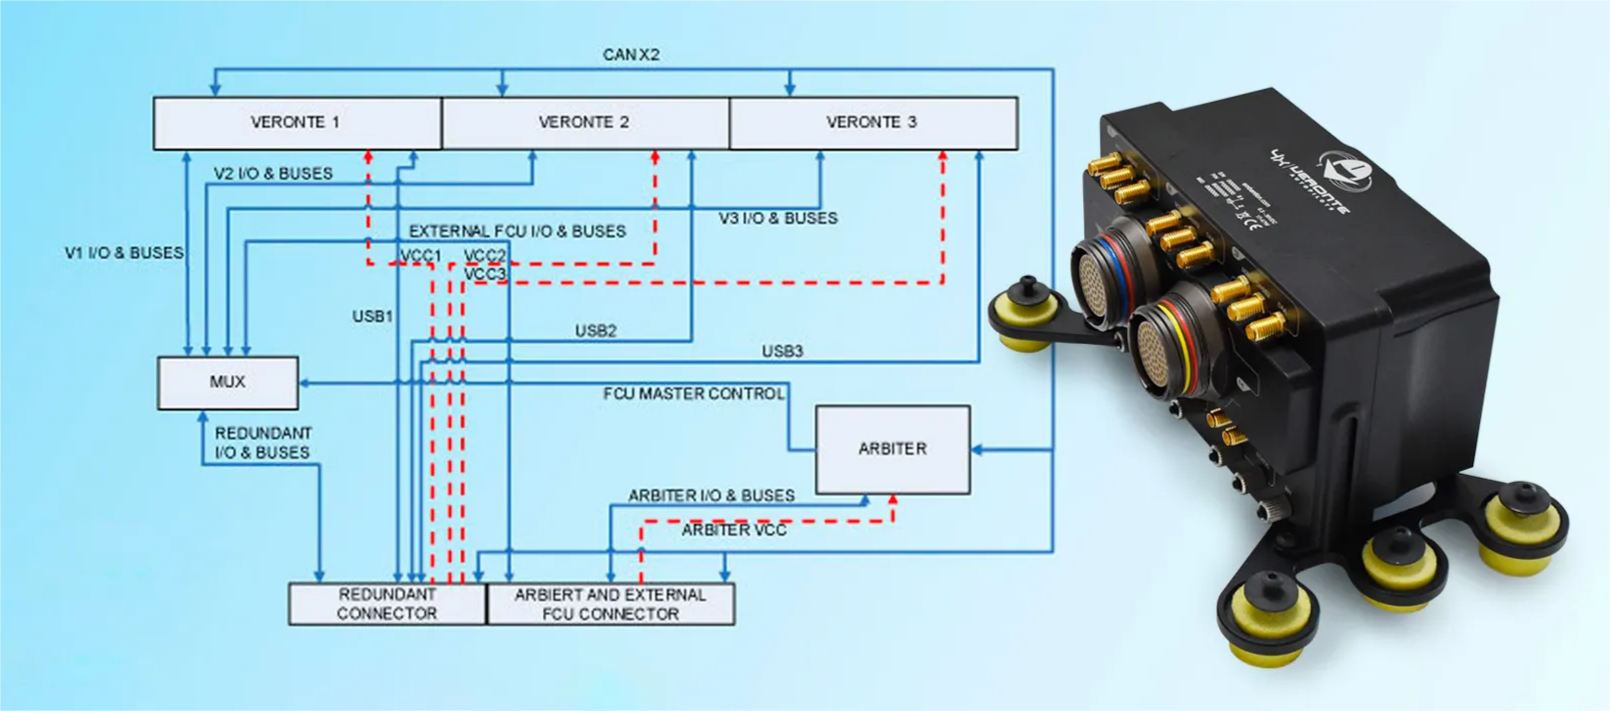
\includegraphics[width=\textwidth]{img/Veronte_Embention.png}
    \caption{Diagrama en bloques del autopiloto Veronte de la empresa Embention. La imagen se extrajo de \cite{embention-2023}.}
    \label{fig:Veronte_Embention}    
\end{figure}

Un detalle que puede verse en este diagrama en bloques es que las computadoras de vuelo se comunican con el árbitro a través de un bus de comunicación. En el sitio web de este autopiloto se menciona que una de las interfaces de comunicación es un bus CAN doble, el cual además puede usarse para la comunicación con motores y sensores. Esto es similar al caso presentado anteriormente en aviones, donde los módulos se comunican a través de un bus de comunicaciones.\\

Vector-600 es una computadora de vuelo con doble redundancia, comercializada por la empresa UAV Navigation \cite{uav-navigation-vector-600}. Esta ofrece redundancia doble en la CPU que realiza los cálculos de actuación y procesamiento de sensores, redundancia doble en la fuente de alimentación y en algunos de los sensores.\\

La empresa MicroPilot ofrece un autopiloto con redundancia triple, MP21283X \cite{wwwmicropilotcom-no-date}. Este se compone de 3 computadoras de vuelo iguales en hardware y software. Durante su uso, la primera de las computadoras de vuelo se encarga de controlar al vehículo. En caso de que esta presente una falla, el autopiloto cambia y utiliza la segunda computadora. Si esta falla, se pasa a la tercera.\\

Estas computadoras de vuelo tienen la particularidad de tener precios muy altos, por ejemplo la primera de ellas de Embention tiene un precio entre 23500 \euro{} y 27000 \euro{}. El presente trabajo busca desarrollar una computadora de vuelo con componentes COTS, por lo que este presupuesto excede la capacidad de este trabajo. Pueden encontrarse una gran cantidad de trabajos que abordan el desarrollo de computadoras de vuelo con redundancias y que utilizan componentes COTS. A continuación se mencionan algunos de ellos.\\

\subsubsection{Casos de Trabajos con Componentes COTS}

En los trabajos \cite{hiergeist2018implementation} y \cite{hiergeist2017internal} los autores presentan una computadora de vuelo redundante, desarrollada con componentes COTS. Esta comprende una redundancia cuádruple utilizando cuatro microcontroladores iguales. Al igual que en el caso del avión comercial y en los autopilotos presentados, la tolerancia a fallas se aborda a partir del intercambio de información. Se utilizan cuatro interfaces SPI, donde en cada una de estas un microcontrolador diferente actúa como master. Los microcontroladores recolectan datos de sensores y realizan un intercambio para ponerse de acuerdo y llegar a un consenso acerca de cuál es el valor correcto. Una vez que esto se decide, se realiza el cálculo de la ley de control. Antes de aplicar el resultado a los motores, se vuelven a comparar resultados para detectar y filtrar fallas. Mientras que en \cite{hiergeist2018implementation} se muestran los resultados, en \cite{hiergeist2017internal} se abordan cuestiones relacionadas al diseño e implementación utilizando componentes COTS. Un aspecto importante de este trabajo es que los cuatro microcontroladores trabajan de manera sincronizada. Los autores mencionan que esto es algo que no puede obviarse, ya que el sistema de control del UAV es un sistema de tiempo real. Para que la tolerancia a fallas funcione adecuadamente, todos los microcontroladores deben procesar datos de sensores que correspondan al mismo ciclo de control. En otras palabras, los 4 nodos de la red redundante realizan la comparación de los datos de sensores al mismo tiempo, realizan el cálculo de la ley de control al mismo tiempo y finalmente vuelven a comparar los resultados al mismo tiempo. En la figura \ref{fig:frame_lock_approach} se muestra un esquema que ejemplifica esto.

\begin{figure}[H]
    \centering
    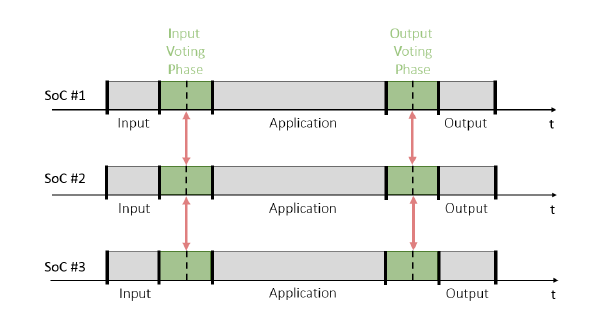
\includegraphics[width=0.6\textwidth]{img/frame_lock_approach.png}
    \caption{Imagen que demuestra la sincronización entre 3 microcontroladores que realizan las mismas tareas en paralelo. La imagen se extrajo de \cite{hiergeist2017internal}.}
    \label{fig:frame_lock_approach}
\end{figure}

Cabe aclarar que la sincronización que se menciona no tiene nada que ver con los osciladores que utiliza cada microcontrolador para su propio funcionamiento. Lo que se sincroniza es el scheduling de las tareas ejecutadas por cada microcontrolador. Por otro lado, esta sincronización no es perfecta ya que sería algo prácticamente imposible. Se acepta que haya cierto desfasaje que no perjudique demasiado el control del vehículo. En \cite{hiergeist2018implementation} se explica la técnica de sincronización utilizada.\\

A diferencia del caso del avión, la comunicación en este trabajo no se realiza por medio de un bus, sino que es a través de 4 interfaces SPI. La justificación de los autores es porque pueden alcanzarse tasas de transferencia de hasta 50 MBit/s, muchísimo mayor que en el bus ARINC 629 que era de 2 MBit/s. Como contrapartida, una conexión SPI requiere de las líneas MOSI, MISO, CS y SCK, además del retorno GND ya que la señal eléctrica de SPI es de modo común. La cantidad de conexiones es mucho mayor que en el caso del uso de un bus. Por ejemplo el autopiloto de Embention utiliza el bus CAN, donde solamente se requieren dos cables, CAN-H y CAN-L. Además, SPI no implementa ningún mecanismo para verificar la integridad del mensaje recibido. Otro aspecto negativo es que el uso de SPI no permite integrar más módulos, como sí sucede en el caso del autopiloto de Embention, donde el mismo bus CAN se utiliza para adosar sensores y actuadores diferentes.\\

En el caso del avión, se había mencionado que el acceso al bus de comunicación era gobernado por el tiempo. En este trabajo además la ejecución del lazo de control y la comparación de resultados también es gobernada por el tiempo.\\

Otro aspecto interesante de este trabajo es que no hay un único elemento que compare los resultados de cada computadora, sino que todas ellas lo hacen. Esto es algo que realiza el autopilot de la empresa Embention mencionado anteriormente. Los autores argumentan que generalmente cuando se utiliza este tipo de árbitro que decide cuál es la computadora de vuelo correcta, esta debe tener una probabilidad de fracaso muy inferior a cada uno de los nodos redundantes, ya que si este árbitro fracasa, todo el sistema fracasará. Esto se muestra en la figura \ref{fig:falla_arbitro}. El árbitro suele ser de un costo muy elevado, algo que se contradice con el requerimiento de que todo el sistema sea desarrollado con componentes COTS.\\

\begin{figure}[H]
    \centering
    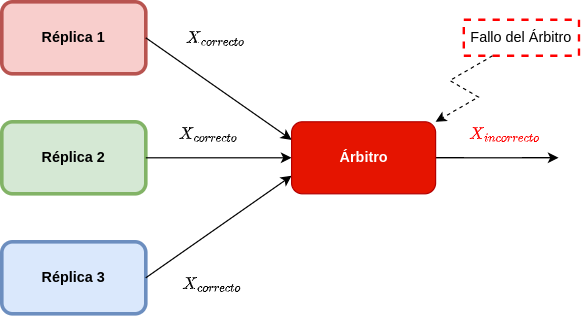
\includegraphics[width=0.5\textwidth]{img/falla_arbitro.png}
    \caption{A pesar de que los 3 módulos redundantes funcionen correctamente, una falla del árbitro se traduce directamente en un error en el sistema. Esto lo vuelve un punto singular de falla.}
    \label{fig:falla_arbitro}
\end{figure}

Una cuestión que no se aclara en este trabajo es cómo se aplican las señales de control a los motores del UAV, ni cómo se recolectan los datos de sensores.\\

En \cite{zhang2020architecture} se presenta otro trabajo desarrollado con componentes COTS. Este también utiliza una arquitectura gobernada por el tiempo. En este trabajo los autores la presentan formalmente con el nombre de \textit{Time-Triggered Architecture}. Esta consiste en que las tareas ejecutadas por el procesador se encuentran predefinidas de forma estática en tiempo de compilación. En este trabajo, al igual que en el caso del avión, se utiliza un bus de comunicación con acceso TDMA, FlexRay \cite{nxpAN12233}. El bus utilizado es doble, para evitar que este sea un punto singular de falla. Al igual que en el trabajo antes mencionado, en este también se implementa una sincronización entre las distintas computadoras de vuelo.\\

La tolerancia a fallas se realiza a través de la comparación de resultados, como en todos los casos presentados hasta el momento. Un aspecto particular de este trabajo es que además de los nodos que realizan los cálculos de ley de control, se incorporan otros microcontroladores extra que se dedican a procesar datos de sensores y de actuadores. Los autores mencionan que esto se hace para alivianar la cantidad de datos enviados a través del bus de comunicaciones y el procesamiento que deben realizar los nodos que calculan la ley de control. Como aspecto negativo, esto encarece a la computadora de vuelo, ya que se requiere una mayor cantidad de procesadores.\\

La sincronización de los nodos redundantes es algo que se repite en varios trabajos encontrados. En \cite{zhang2015dual} se presenta un desarrollo de una computadora de vuelo para pequeños UAVs, con redundancia doble y sincronización en la ejecución de las tareas. La redundancia también se administra a través de la comparación de entradas de sensores y resultados de cálculos de la ley de control. En la figura  \ref{fig:FCC_dual_FPGA} se muestra un diagrama en bloques. Si bien ambas computadoras trabajan en paralelo, solo una de ellas es la que controla los actuadores. 

\begin{figure}[H]
    \centering
    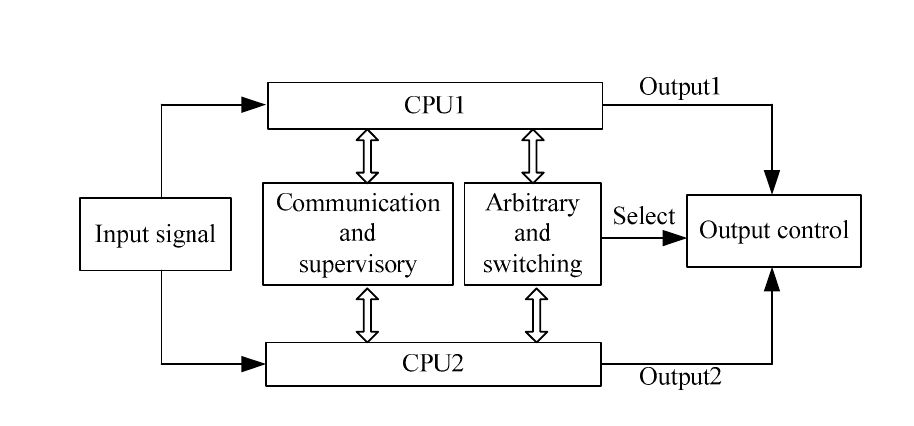
\includegraphics[width=0.7\textwidth]{img/FCC_dual_FPGA.png}
    \caption{Diagrama en bloques del sistema de redundancia doble. Las CPU1 y CPU2 comparan sus resultados y envían sus salidas al bloque \textit{Output control}. A través de un bloque árbitro se selecciona a cuál de las dos CPU será la que controle los actuadores. La imagen se extrajo de \cite{zhang2015dual}.}
    \label{fig:FCC_dual_FPGA}
\end{figure}

En caso de que ocurra una discrepancia entre los resultados de ambas, eso indicará que alguna de las dos computadoras cometió un error, pero no se sabrá cuál fue. Luego de ejecutar una serie de rutinas se verifica cuál de las 2 cometió el error y en caso de que sea necesario, se le pasa el control de los actuadores a la computadora de back-up.\\

Un aspecto negativo de esta configuración es el hecho de que la comparación de resultados no permite identificar cuál de las dos CPUs cometió el error, solamente se puede saber que ocurrió un error. Pensando en que la ejecución del lazo de control es un sistema de tiempo real, sería deseable que a pesar de la falla, el sistema de control pueda seguir ejecutándose. El hecho de tener que ejecutar rutinas para verificar a la computadora fallada presenta un trabajo que perjudica el control del vehículo. Esto es algo que no sucede por ejemplo, si se utilizan 3 computadoras de vuelo en paralelo, ya que si una presenta un dato incorrecto, simplemente puede ignorarse el dato y utilizar los datos de las otras 2 computadoras correctas. Esto se denomina \textit{fault masking} o enmascaramiento de la falla.\\

En \cite{chen2015design} y \cite{wang2008development} pueden encontrarse otros 2 trabajos más que utilizan la sincronización entre los nodos redundantes. El primero de ellos trabaja con redundancia triple y un árbritro que selecciona cuál de los nodos controla los actuadores. El segundo también trabaja con redundancia triple, pero no utiliza un árbitro sino que las tres computadoras realizan la votación y cada una de ellas envía un mensaje a un nodo que se encuentra en el mismo bus y se encarga de controlar el actuador. En la figura \ref{fig:RS_485_sync} se muestra el diagrama en bloques.

\begin{figure}[H]
    \centering
    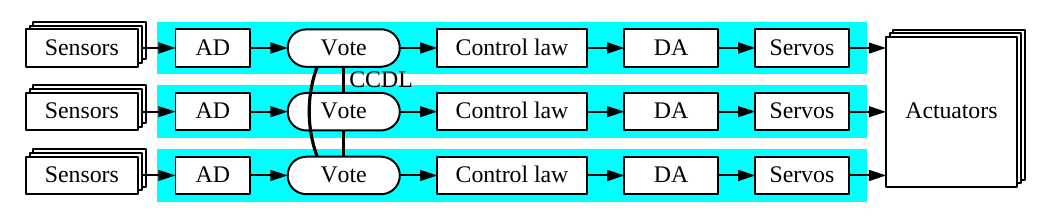
\includegraphics[width=\textwidth]{img/RS_485_sync.png}
    \caption{Diagrama en bloques del sistema redundante de \cite{wang2008development}. Cada uno de los nodos tiene sus propios sensores, la única comunicación que se realiza a través del bus CCDL (\textit{Cross-Communication Data Link}) es para realizar la comparación de resultados y la votación.}
    \label{fig:RS_485_sync}
\end{figure}

En \cite{thesis_redundant_ROS} se presenta un trabajo de tesis en el que no se utiliza una sincronización entre los nodos. Este consiste en la utilización de 2 computadoras de vuelo de fácil acceso comercial, PixHawk \cite{dronecode-foundation-2023}, conectadas a una tercera computadora de vuelo central implementada con una Raspberry Pi que funciona como árbitro. En la figura \ref{fig:ROS_redundancy} se muestra un diagrama en bloques de esta arquitectura. La técnica utilizada consiste en que el árbitro continuamente le pide a ambas computadoras información acerca de su ``estado de salud''. A partir de la información recibida de ambas, el árbitro controla unas llaves implementadas como relés de estado sólido que seleccionan cuál de las 2 comptuadoras será la que controle los motores.

\begin{figure}[H]
    \centering
    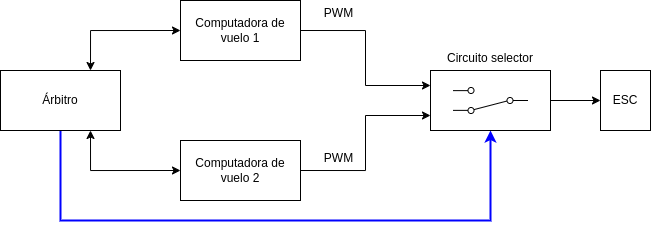
\includegraphics[width=0.7\textwidth]{img/ROS_redundancy.png}
    \caption{Arquitectura de la computadora de vuelo utilizada en \cite{thesis_redundant_ROS}. El árbitro selecciona cuál de las dos señales PWM se utiliza para controlar el \textit{Electronic Speed Controller} (ESC).}
    \label{fig:ROS_redundancy}
\end{figure}

Un aspecto que no se menciona en este trabajo es cómo se administra el switcheo de los relés. Teniendo en cuenta que este switcheo puede traer consigo un cambio brusco en la señal PWM que ven los actuadores de los motores, habrá un período de reestabilización del lazo de control. Este requiere un análsis detallado que asegure que no se pierda el control del vehículo.




%\textbf{{\color{red} COMPLETAR}}

\section{Requerimientos de un Sistema con Tolerancia a Fallas}\label{sec:requerimentos_sistema_tolerancia_fallas}

A partir de los distintos casos presentados, en esta sección se busca relevar cuáles son las características comunes en sistemas con tolerancia a fallas. Se analizan las distintas alternativas y luego se mencionan los criterios tenidos en cuenta para el desarrollo de la computadora de vuelo. En este trabajo no se define a priori cuál es la arquitectura del sistema en cuanto al uso de redundancias, por lo que la computadora de vuelo debe tener cierta diversidad en cuanto a sus capacidades.\\

\subsection{Requerimientos Comunes en Sistemas con Redundancias}

Todos los trabajos y ejemplos presentados en la sección anterior comparten la característica de implementar la tolerancia a fallas utilizando varias copias del mismo elemento de hardware. Estas copias trabajan en paralelo y se comparan los resultados obtenidos por cada una de ellas. Las fallas se detectan cuando ocurre una diferencia en los resultados de las copias.\\

{\color{red} EXPLICAR Y JUSTIFICAR EL POR QUÉ DE LAS REDUNDANCIAS POR SOBRE EL USO DE COMPONENTES DE ALTÍSIMA CALIDAD, EN UN PÁRRAFO.}

A continuación, se describen algunas de las características detectadas.

\subsubsection{Sincronismo de los Nodos}
%\subsection{Sincronismo de los Nodos}

Prácticamente en todos los trabajos presentados se menciona que los nodos reundantes trabajan de manera sincronizada. Esta necesidad surge debido a que las comparaciones se realizan sobre variables que cambian en el tiempo y que tienen validez solamente durante un período de tiempo. Esto es algo característico de sistemas de tiempo real, ya que un dato de un sensor $X(t)$ solamente tendrá validez durante un breve período de tiempo. 
%En las arquitecturas antes presentadas, se menciona que se realiza una comparación de los resultados calculados por cada nodo, para detectar/enmascarar errores. Para que el funcionamiento de esta comparación sea adecuado, los nodos deben estar sincronizados. Esto es un requerimiento para sistemas de tiempo real, como el caso de la computadora de vuelo de un UAV.
En la figura \ref{fig:3_4_1_sincronizacion} se muestra un ejemplo. En el instante $t$, se presenta una nueva medición de un sensor a las tres computadoras de vuelo. Al comienzo de la misión, todas ellas estarán sincronizadas y generarán un resultado del cálculo de la ley de control que corresponde al mismo intervalo de tiempo. Luego, se realiza la votación para elegir el valor correcto. La figura \ref{fig:3_4_1_sincronizacion_2}, muestra lo que sucede al cabo de un período de tiempo. Se presenta una nueva medición de un sensor en el instante $t$. Debido a la desincronización, es posible que las computadoras de vuelo no presenten sus resultados al árbitro a tiempo, por lo que este asumirá que una de las FCCs no presentó ninguna respuesta. Este caso suele estar contemplado dentro de las posibilidades y correpsonde al caso en el que una computadora de vuelo presentó un error y debido a ello no respondió con ningún valor (por ejemplo, se reinició su procesador debido a un \textit{watchdog}). En esos casos el árbitro simplemente asume algún valor por defecto.

\begin{figure}[H]
    \centering
    \begin{subfigure}[b]{0.49\textwidth}
        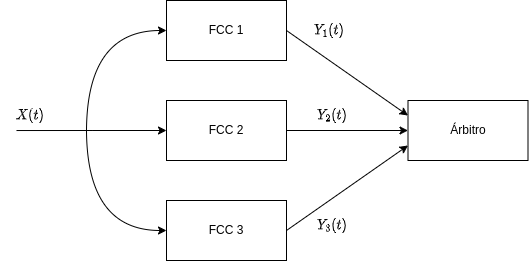
\includegraphics[width=\textwidth]{img/3_4_1_sincronizacion_1.png}
        \caption{Computadoras de vuelo al inicio de la misión.}
        \label{fig:3_4_1_sincronizacion_1}
    \end{subfigure}
    \begin{subfigure}[b]{0.49\textwidth}
        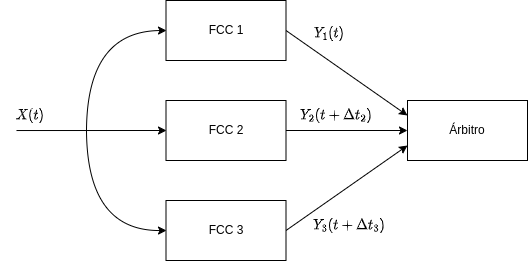
\includegraphics[width=\textwidth]{img/3_4_1_sincronizacion_2.png}
        \caption{Al cabo de un período de tiempo, se desincronizarán.}
        \label{fig:3_4_1_sincronizacion_2}
    \end{subfigure}
    \caption{A medida que transcurra el tiempo, la desincronización entre FCCs impactará en el sistema redundante.}
    \label{fig:3_4_1_sincronizacion}
\end{figure}

Otra situación que puede presentarse, es que los resultados propuestos por las computadoras de vuelo $Y_1$, $Y_2$ e $Y_3$ correspondan a intervalos de tiempo distintos. Este caso es todavía peor que el anterior, ya que no se encuentra contemplado y el árbitro simplemente realizará la votación asumiendo que el dato es válido.

\begin{figure}[H]
    \centering
    \begin{subfigure}[b]{0.49\textwidth}
        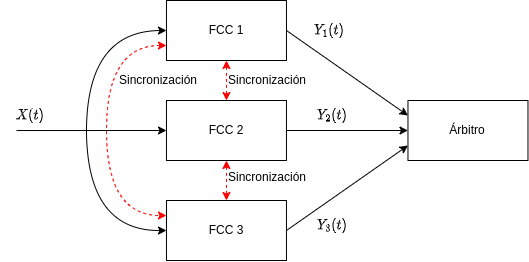
\includegraphics[width=\textwidth]{img/3_4_1_sincronizacion_3.png}
        \caption{Las mismas computadoras de vuelo se encargan de la sincronización.}
        \label{fig:3_4_1_sincronizacion_3}
    \end{subfigure}
    \begin{subfigure}[b]{0.49\textwidth}
        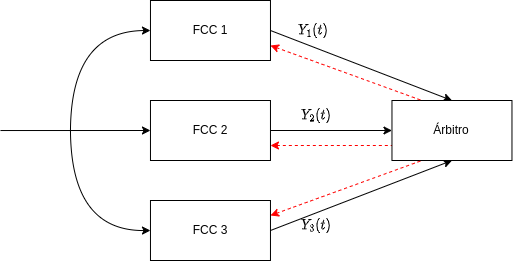
\includegraphics[width=\textwidth]{img/3_4_1_sincronizacion_4.png}
        \caption{En este caso, la sincronización es administrada por el árbitro.}
        \label{fig:3_4_1_sincronizacion_4}
    \end{subfigure}
    \caption{La sincronización entre nodos es necesaria para un correcto funcionamiento de las redundancias.}
\end{figure}

Se concluye que es mandatorio utilizar alguna técnica de sincronización entre los nodos. Como detalle de la figura \ref{fig:3_4_1_sincronizacion_3}, se muestra que la sincronización entre nodos presupone otro canal de comuniación más. Otra forma podría ser relegar la tarea de la sincronización al árbitro, aunque esto nuevamente presenta un punto singular de falla. Como se demostró en esta sección, el sincronismo es un aspecto crítico en el sistema redundante, por lo que se prefiere evitar esto último. Aunque de todas formas quisiera relegarse la sincronización al árbitro, este no solo recibirá mensajes de cada una de las FCCs, sino que además les enviará mensajes. Esto se muestra en la figura \ref{fig:3_4_1_sincronizacion_4}. Puede ocurrir una situación en la que el árbitro entregue valores distintos a cada una de las FCCs, evitando que estas se sincronicen.

\subsubsection{Consenso}\label{sec:consenso}
%\subsection{Consenso}\label{sec:consenso}

Como se mostró en la figura \ref{fig:3_4_1_sincronizacion_3}, las computadoras de vuelo pueden comunicarse entre ellas para lograr una sincronización, por ejemplo compartiendo a sus pares un valor asociado a su propio clock interno. Cada FCC propone un valor distinto y estas buscarán ponerse de acuerdo en un valor único. Para que cada una de ellas llegue a la misma conclusión acerca del valor de clock correcto, si todas ellas ejecutan el mismo algoritmo y poseen los mismos valores de entrada, luego llegarán a la misma conclusión. En la figura \ref{fig:3_4_2_consenso_4} se muestra un caso en el que una de las computadoras de vuelo comparte valores de clock distintos a sus pares.

\begin{figure}[H]
    \centering
    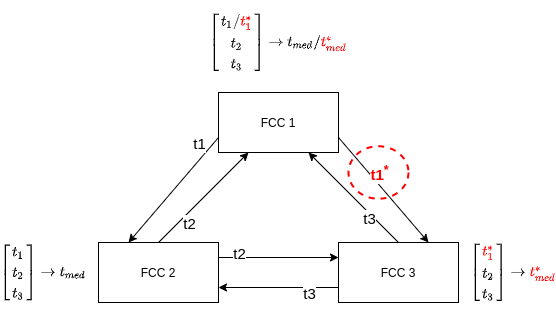
\includegraphics[width=0.6\textwidth]{img/3_4_2_consenso_4.png}
    \caption{La FCC1 entrega un valor distinto de timing a las demás FCCs}.
    \label{fig:3_4_2_consenso_4}
\end{figure}

En este escenario, la FCC1 entrega dos valores distintos de su clock a las demás FCCs. Cada una de ellas luego realiza un promedio para llegar a un único valor. Lo que se observa es que las FCC2 y FCC3 calcularán un valor promedio distinto, es decir, no se sincronizarán.
Una posible solución podría ser que las FCCs hagan un nuevo intercambio, con los valores promedio calculados y realicen una votación interna. Esto se muestra en la figura \ref{fig:3_4_2_consenso_5}.

\begin{figure}[H]
    \centering
    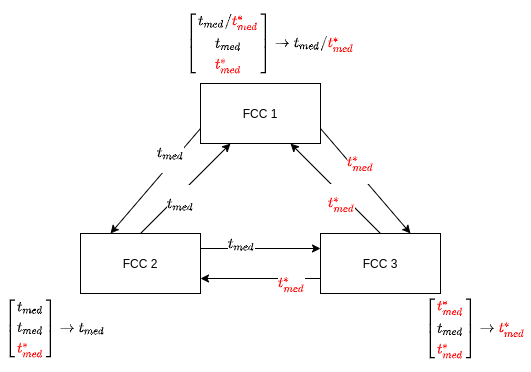
\includegraphics[width=0.6\textwidth]{img/3_4_2_consenso_5.png}
    \caption{Luego de calcular los promedios, las FCCs intercambian sus resultados. Nuevamente, la FCC1 comete una falla en el envío del dato.}
    \label{fig:3_4_2_consenso_5}
\end{figure}

Esta última situación, donde la FCC1 nuevamente comparte dos valores distintos a las demás, puede llevar a que las computadoras de vuelo no se sincronicen, algo que como ya se mencionó, es crítico para la correcta ejecución del algoritmo de tolerancia a fallas. Podría argumentarse que es demasiado pesimista pensar que la FCC1 puede producir la misma falla 2 veces de manera consecutiva, ya que existe una baja probabilidad de que ello suceda. Sin embargo, la situación planteada en esta sección puede tratarse como un tipo de falla de hardware que se manifiesta como comportamientos arbitrarios. Que exista una sincronización entre nodos redundantes implica que estos llegan a un consenso del paso del tiempo y el ritmo al que deben ejecutar sus tareas asignadas. Este consenso resulta crítico para que el sistema pueda detectar fallas correctamente.\\

Algunos de los trabajos presentados anteriormente además realizan el algoritmo de votación sin la inclusión de un árbitro. Este caso es idéntico al de la figura \ref{fig:3_4_2_consenso_4}, es decir que el mismo problema del consenso también está presente para las votaciones acerca de resultados de cálculo de ley de control.\\

El modelo de falla que se está considerando representa un comportamiento anómalo arbitrario, es decir, que a priori no se asume nada acerca de la falla. A este tipo de comportamiento se lo denomina falla bizantina o \textit{Byzantine Fault} en inglés y básicamente consiste en asumir que el elemento que manifiesta la falla presenta un comportamiento arbitrario. Por ejemplo, un sensor puede dejar de funcionar repentinamente y no dar más respuesta, puede dejar de enviar respuesta por un período de tiempo y luego volver a funcionar, podría también enviar datos a un microcontrolador pero que esos datos sean incoherentes, etc. El modelo de falla bizantina no asume modos de falla, sino que el comportamiento es arbitrario \cite{roth2021not}\cite{hiergeist2017internal}\cite{lala1994architectural}. El nombre proviene de un problema denominado \textit{The Byzantine Generals Problem}, formalizado en \cite{lamport2019byzantine}. Otros trabajos que tratan el mismo problema son \cite{pease1980reaching} y \cite{wensley1978sift}. Este último, presenta el diseño de una computadora de vuelo tolerante a fallas que utiliza los resultados del \textit{Byzantine Generals Problem} para realizar distintas tareas de redundancia.\\

%Una forma de alivianar esta tarea es la de considerar un modelo de falla de hardware más conservador, donde se asume que una falla de hardware consiste en que esta presente un comportamiento anómalo arbitrario, es decir, de cualquier tipo. A este tipo de comportamiento se lo denomina falla bizantina o \textit{Byzantine Fault} en inglés y básicamente consiste en asumir que el elemento que manifiesta la falla presenta un comportamiento arbitrario. Por ejemplo, un sensor puede dejar de funcionar repentinamente y no dar más respuesta, puede dejar de enviar respuesta por un período de tiempo y luego volver a funcionar, podría también enviar datos a un microcontrolador pero que esos datos sean incoherentes, etc. El modelo de falla bizantina no asume modos de falla, sino que el comportamiento es arbitrario \cite{roth2021not}\cite{hiergeist2017internal}\cite{lala1994architectural}. Se define un sistema tolerante a este tipo de fallas.

Se plantea una situación como la de la figura \ref{fig:3_4_2_consenso_4}, pero en este caso se utilizan 4 computadoras de vuelo en lugar de 3. En este caso, las computadoras de vuelo deben sincronizarse. Para lograrlo, ellas comparten un valor de timestamp, que pueden utilizar para ajustar sus clocks. En la figura \ref{fig:Byzantine_Generals_Problem_5} se muestra un escenario en el que una de las computadoras de vuelo presenta una falla tal que le informa un valor distinto a cada una de sus pares.

\begin{figure}[H]
    \centering
    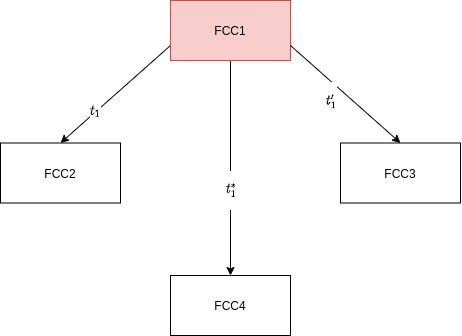
\includegraphics[width=0.5\textwidth]{img/Byzantine_Generals_Problem_5.png}
    \caption{Debido a una falla, la computadora de vuelo 1 le entrega valores distintos de timestamp a las demás.}
    \label{fig:Byzantine_Generals_Problem_5}
\end{figure}

\begin{figure}[H]
    \centering
    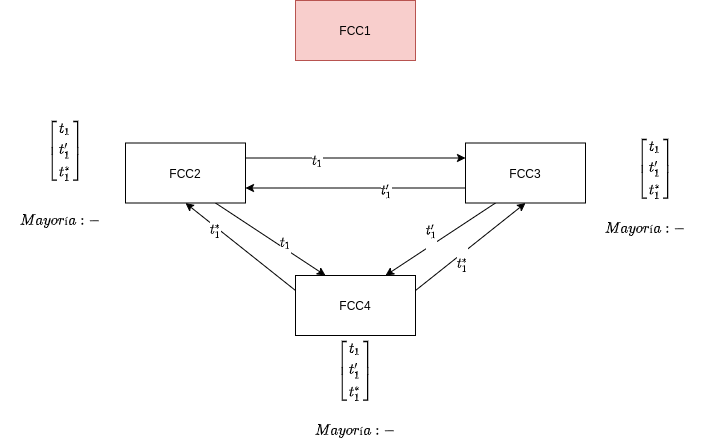
\includegraphics[width=0.7\textwidth]{img/Byzantine_Generals_Problem_6.png}
    \caption{Las FCC2, 3 y 4 comparten entre sí lo que les dijo la FCC1 a cada una y llegan a la conclusión de que la información es inconsistente.}
    \label{fig:Byzantine_Generals_Problem_6}
\end{figure}

A través de un segundo intercambio, las FCC 2, 3 y 4 llegan a la conclusión de que el timestamp de la FCC1 no es claro. En este caso, descartan el valor. Luego de hacer todos los intercambios de timestamp, las FCCs podrán aplicar internamente la sincronización, por ejemplo, calculando un promedio de todos los timestamp. \textbf{Dado que todas las FCCs tendrán la misma información de timestamp entregado por las demás FCCs, luego todas llegarán al mismo promedio y se sincronizarán}.\\

Un aspecto interesante es el hecho de que en el paper original, se hace una analogía entre un nodo redundante con fallas y un nodo traidor, es decir, que busca corromper el consenso de los demás nodos. Esto lo que quiere decir es que las fallas presentadas por las computadoras de vuelo pueden ser justamente de cualquier característica, incluso al extremo de presentar un comportamiento malicioso, con el objetivo de perjudicar al sistema \cite{lala1994architectural}. Esto sienta las bases para la tolerancia a fallas de hardware arbitrarias.\\

La implementación del algoritmo tolerante a fallas arbitrarias resulta costoso. Para poder tolerar fallas provenientes de 1 FCC se requiere un total de 4 computadoras de vuelo. Además, debe haber una interconexión entre las 4 computadoras y ellas deben intercambiar información continuamente para poder detectar y enmascarar la falla. A todo esto se le debe sumar, la necesidad de la sincronización.\\

\subsection{Simplificación del Problema}

Una de las cuestiones que no se menciona en el problema original, es el caso en el que los nodos constituyen sistemas de tiempo real. Las computadoras de vuelo deben realizar tareas que requieren determinismo temporal, por ejemplo cálculo de la ley de control, estimación de la pose, etc... En el problema original, los nodos pueden enviar sus mensajes a sus pares en cualquier momento y en cualquier orden. Otro de los puntos que caracterizan al problema original, es el hecho de que la comunicación entre los nodos es 1 a 1. Debido a esto, los traidores pueden entregar información confusa a sus pares para tratar de romper el consenso. Esto es lo que vuelve complejo al problema \cite{lamport2019byzantine} y costosa a su solución \cite{roth2021not}. Si el sistema en cuestión presenta la características de ser de tiempo real e implementar una comunicación a través de un bus, en conjunto, luego el problema del consenso puede simplificarse mucho.\\

En sistemas de tiempo real para aplicaciones \textit{safety-critical}, es común encontrar sistemas distribuidos con comunicación a través de un bus. Esto se mencionó en la sección \ref{sec:estado_del_arte} tanto para el caso del avión como para varios de los ejemplos de UAVs presentados. Esto tambień ocurre por ejemplo en los automóviles, los nodos que se encuentran repartidos por todo el vehículo se comunican a través de redes como CAN\cite{specification1991bosch} o FlexRay\cite{nxpAN12233}. Todos los nodos de la red se encuentran conectados al mismo bus de comunicación, por lo que cuando un nodo envía un mensaje a través del bus, todos los demás nodos reciben el mismo mensaje.

\begin{figure}[H]
    \centering
    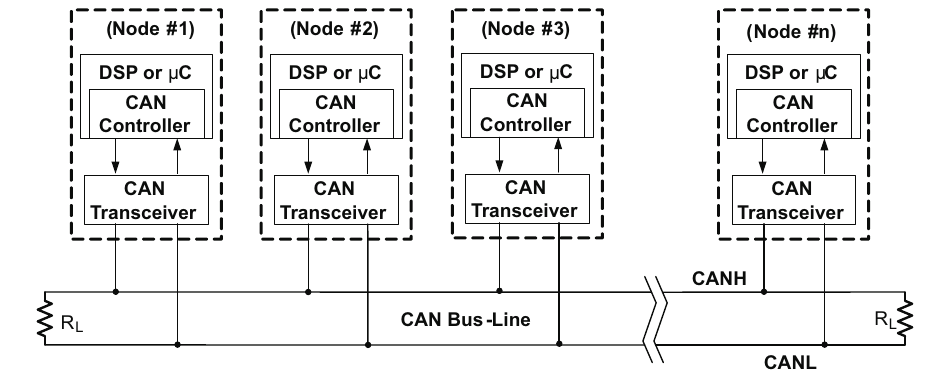
\includegraphics[width=\textwidth]{img/red_CAN.png}
    \caption{Todos los nodos se encuentran conectados al mismo bus de comunicaciones. En el caso del bus CAN, se compone de dos cables, CAN-H y CAN-L, terminados en sus extremos por resistencias de adaptación. La imagen se extrajo de \cite{texasSLOA101B}.}
    \label{fig:red_CAN}
\end{figure}

Esto presenta una diferencia respecto de lo planteado en \textit{The Byzantine Generals Problem}, ya que la existencia de un bus común a todos los nodos automáticamente elimina la posibilidad de que uno de los miembros de la red pueda enviar información diferente a sus pares. Puede compararse la figura \ref{fig:byzantine_bus_1} con la figura \ref{fig:Byzantine_Generals_Problem_5}.

\begin{figure}[H]
    \centering
    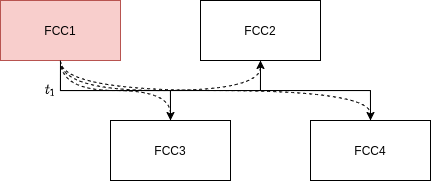
\includegraphics[width=0.6\textwidth]{img/byzantine_bus_1.png}
    \caption{En este caso, la conexión tipo bus no permite el envío de información diferente a los demás miembros. La FCC1 envía el valor $t_1$ y todos sus pares reciben el mismo valor.}
    \label{fig:byzantine_bus_1}    
\end{figure}

Como contrapartida, debido a que los nodos comparten canal de comunicación, estos deben tomar turnos para enviar la información a sus pares. De otra forma, habría una colisión en el bus y la información nunca llegaría a su destino. Sumado a esto, el bus se convierte en un punto singular de falla, ya que es posible que un problema en el bus deje a los nodos incomunicados.\\

%\subsubsection{Consenso}

Al igual que como se hizo en la sección \ref{sec:consenso}, se analiza el problema del consenso utilizando un bus. El ejemplo que se presentó anteriormente fue el necesario para lograr una sincronización entre las FCCs y se mostró que el enviar información distinta a cada computadora de vuelo puede romper el sincronismo muy fácilmente.\\

Como ya se mencionó, las FCCs deben tomar turnos para utilizar el medio físico. En las próximas secciones se explicará cómo se puede lograr esto, aquí se asume que las FCCs respetan sus turnos para utilizar el medio físico compartido. En la figura \ref{fig:byzantine_bus_2}, la FCC1 accede al medio y envía su valor de timestamp. Las demás FCCs reciben el mismo valor, por estar conectadas al mismo bus de comunicación. Luego, las FCC2 y 3 repiten esto mismo. En la figura \ref{fig:byzantine_bus_3} se muestra que todas tienen la misma información respecto de sus pares. Luego por ejemplo, si calculan un promedio, llegarán al mismo resultado y se sincronizarán correctamente.

\begin{figure}[H]
    \centering
    \begin{subfigure}[b]{0.34\textwidth}
        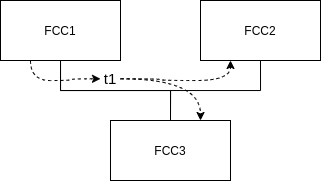
\includegraphics[width=\textwidth]{img/byzantine_bus_2.png}
        \caption{La FCC1 envía su \textit{timestamp} hacia las demás.}
        \label{fig:byzantine_bus_2}
    \end{subfigure}\hfill
    \begin{subfigure}[b]{0.49\textwidth}
        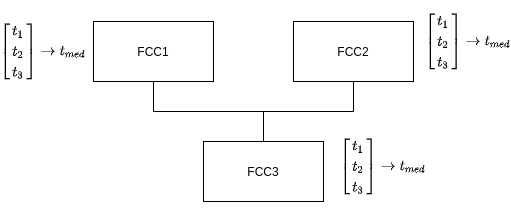
\includegraphics[width=\textwidth]{img/byzantine_bus_3.png}
        \caption{Luego de finalizar los intercambios, todas las FCCs llegan al mismo resultado de \textit{timestamp} para sincronizarse.}
        \label{fig:byzantine_bus_3}
    \end{subfigure}
    \caption{Debido a la existencia del bus, las FCCs no pueden mentir acerca de su \textit{timestamp}. Luego, todas llegan a un consenso de manera casi trivial.}
    \label{}
\end{figure}

A partir de este análisis, se puede ver que para el caso de un sistema de tiempo real con un único bus de comunicaciones, el problema del consenso es mucho más sencillo que lo que se muestra en \textit{The Byzantine Generals Problem}. De todas maneras, lo que se presenta aquí es un primer análisis, ya que se ha asumido que no hay colisiones en el bus y que los nodos se encuentran sincronizados. Se concluye que, para que la computadora de vuelo pueda implementar distintos mecanismos de tolerancia a fallas, esta debe contar con una interfaz que le permita la comunicación a través de un bus de comunicaciones.\\

\subsection{Uso de Componentes COTS}

\textbf{{\color{red} COMPLETAR}}

\subsection{Selección del Bus de Comunicaciones de la Computadora de Vuelo}

Como ya fue mencionado, la computadora de vuelo requiere de una interfaz para un bus de comunicaciones. A partir de lo presentado hasta aquí el único requerimiento es el método de acceso al medio, el cual debe ser controlado por el tiempo. Teniendo en cuenta que se trata de un trabajo realizado con componentes COTS, el hardware a utilizar debe ser de fácil acceso y con costos razonables. Para el desarrollo de este trabajo, se seleccionó el bus \textit{Controller Area Network} (CAN)\cite{specification1991bosch}. 

%En las secciones siguientes se explica un inconveniente, en cuanto a la selección del microcontrolador. 

El microcontrolador que se utiliza cuenta con un periférico que permite utilizar una interfaz con este bus. A continuación se presentan brevemente algunas características. Si bien el método de acceso al medio no es TDMA, existe una extensión del protocolo que justamente busca incorporar esta funcionalidad en otra capa superior.

\subsubsection{Descripción del Protocolo CAN}

El protocolo CAN fue desarrollado para ser usado en la industria automotriz, como bus de comunicación que conecta distintos módulos dentro de un automóvil. El objetivo de su desarrollo fue similiar al motivo por el cual se desarrolló el bus ARINC 629, reemplazar la gran cantidad de cables dentro del vehículo por un bus simple. El protocolo se corresponde con el modelo OSI y la especificación original define las capas física y de enlace, ISO 11898.\\

Cada nodo de un bus CAN se conecta a este a través de 2 cables, los cuales llevan la señal diferencial. Esto se muestra en la figura \ref{fig:conxeion_al_bus_CAN}. Todo el bus CAN se compone de 2 cables que llevan los mensajes a todos los nodos de la red. El hecho de que se trate de una señal diferencial hace que la comunicación sea robusta, reduciendo las emisiones electromagnéticas generadas por este. A su vez, es común que el bus sea cableado como un par trenzado, lo que atenúa señales de modo común, producto de cualquier acoplamiento. 

\begin{figure}[H]
    \centering
    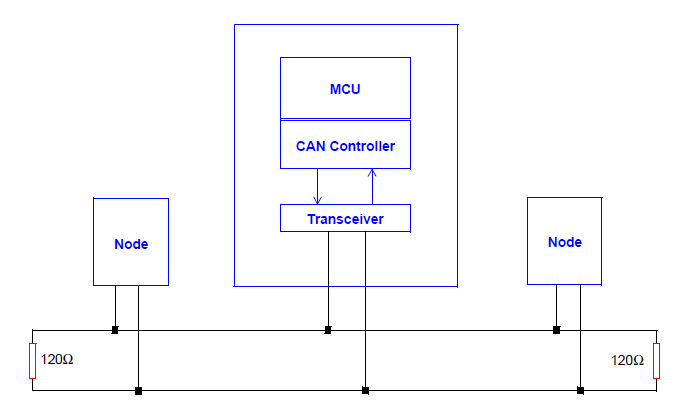
\includegraphics[width=0.5\textwidth]{img/conxeion_al_bus_CAN.png}
    \caption{La conexión de un nodo al bus es a través de 2 cables que llevan dos señales, CAN-H y CAN-L. La imagen se extrajo de \cite{AN228}.}
    \label{fig:conxeion_al_bus_CAN}    
\end{figure}

Existen muchas versiones del protocolo CAN, en este trabajo se utiliza la versión CAN High Speed. Esta define una velocidad máxima de transferencia de 1 Mbps, para un bus de hasta 40 m de longitud y 30 nodos conectados al mismo bus. Se recomienda que la conexión entre cada nodo y el bus no sea de más de 30 cm. El hecho de poder tener hasta 30 nodos expande las posibilidades de uso del bus, más allá de ser el medio principal de comunicación utilizado para el sistema redundante. Por ejemplo, distintos sensores o incluso actuadores como los motores del vehículo podrían conectarse al bus. {\color{red} Acá tendría que agregar alguna referencia a este uso del bus CAN}.\\

La impedancia característica del bus debe ser de $120 \ \Omega$. Es común agregar resistores de terminación en ambos extremos, para evitar reflexiones. En algunos casos pueden llegar a encontrarse aplicaciones donde los resistores de terminación se incluyen dentro de alguno de los nodos del bus. Esto no es recomendable, ya que si este se desconecta de forma accidental del bus, todas las comunicaciones entre los demás nodos se verán perjudicadas.\\

En la figura \ref{fig:conxeion_al_bus_CAN} se muestran 2 elementos que forman parte del nodo, el \textit{trasnciever} y el \textit{controller}. El primero de ellos forma parte de la capa física y es un circuito que convierte las señales diferenciales del bus en señales de modo común, que luego son transferidas al elemento \textit{controller}. Este componente sirve como interfaz física con el bus.\\

CAN es un protocolo donde no hay un nodo master, sino que todos pueden utilizar el medio para transmitir mensajes, mientras el bus no esté en uso. El método de acceso al medio que se utiliza es \textit{Carrer Sense Multiple Access with Collision Detection and Arbitration on Message Priority} (CSMA/CD+AMP). Antes de transmitir un mensaje, el nodo sensa el medio físico y en caso de que esté libre, intenta utilizarlo. En caso de que más de un nodo quiera enviar un mensaje a la vez, la colisión se detcta a través de un campo de la trama CAN, el campo ID. Se definen 2 tipos de tramas, estándar, figura \ref{fig:CAN_frame_standard} y extended, figura \ref{fig:CAN_frame_extended}.

\begin{figure}[H]
    \centering
    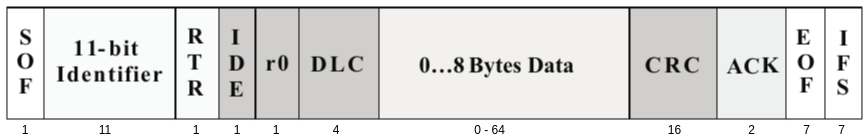
\includegraphics[width=0.8\textwidth]{img/CAN_frame_standard.png}
    \caption{Se muestran los campos de una trama CAN estándar. Debajo de cada campo se indica la cantidad de bits. La imagen se extrajo de \cite{texasSLOA101B}.}
    \label{fig:CAN_frame_standard}
\end{figure}


\begin{figure}[H]
    \centering
    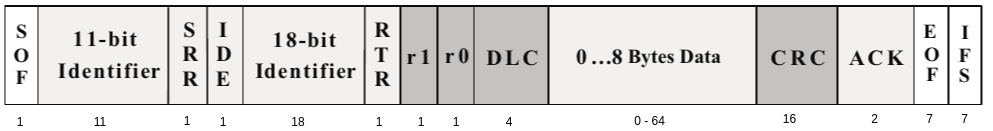
\includegraphics[width=0.8\textwidth]{img/CAN_frame_extended.png}
    \caption{Se muestran los campos de una trama CAN extendida. Debajo de cada campo se indica la cantidad de bits. La imagen se extrajo de \cite{texasSLOA101B}.}
    \label{fig:CAN_frame_extended}
\end{figure}

En el eventual caso en que más de un nodo detecte el medio sin uso, estos querrán transmitir a través del bus. Esta situación se encuentra contemplada por el protocolo y se implementa un mecanismo que resuelve la colisión asegurando la transmisión del mensaje con la prioridad más baja. El primer bit es el campo SOF, seguido del identificador. En la figura \ref{fig:CAN_arbitration} se muestra un ejemplo de este escenario. Tanto el nodo 1 como el nodo 2 quieren utilizar el bus CAN. Ambos comienzan a inyectar su ID correspondiente. En algún momento, ocurre una discrepancia entre el ID inyectado por ambos nodos. Aquel con el campo dominant, es decir 0, gana y completa su transmisión, en este caso el nodo 2. El nodo 1 que quiso envar un 1 por su lado, detecta un 0. Esto genera que detenga su transmisión, dejando que los demás nodos utilicen el medio.

\begin{figure}[H]
    \centering
    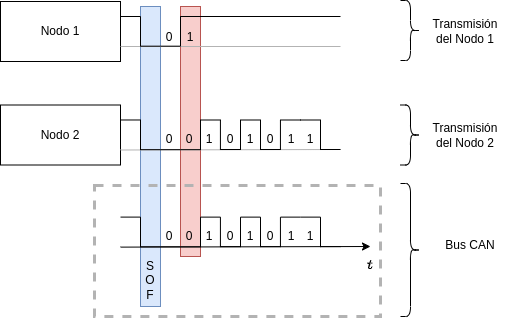
\includegraphics[width=0.6\textwidth]{img/CAN_arbitration.png}
    \caption{Mecanismo para la detección de colisiones. El nodo 2 gana por prioridad y completa su transmisión, mientras que el nodo 1 deja de usar el bus, aguardando a que el nodo 2 finalice.}
    \label{fig:CAN_arbitration}
\end{figure}

En las figuras \ref{fig:CAN_frame_standard} y \ref{fig:CAN_frame_extended} se puede ver que las tramas tienen un campo CRC, el cual es utilizado para que el receptor pueda verificar la integridad del mensaje. Además, se muestra otro campo, el ACK. Cada vez que un nodo recibe un mensaje correctamente, este sobreescribe el bit de ACK con un dominant, es decir un 0.\\

El protocolo CAN base no tiene un acceso al medio controlado por el tiempo, sino que es dominado por eventos (\textit{event-triggered}), ya que varios nodos pueden querer transmitir varios mensajes a la vez, de manera consecutiva. En el estándar ISO 11898-4\cite{ISO11898_4} se define una extensión denominada \textit{Time-Triggered CAN} (TTCAN). A través de una capa de sesión, puede implementarse un acceso al medio dominado por el tiempo.\\

Como se mencionó al principio de la sección \ref{sec:requerimentos_sistema_tolerancia_fallas}, la arquitectura para la tolerancia a fallas no está definida. La elección del protocolo CAN le da versatilidad al uso del bus, ya que puede utilizarse con un acceso al medio tanto controlado por el tiempo como por eventos.

\section{Diseño y Construcción de la Computadora de Vuelo}

% Acá se da una introducción breve de esta sección, es decir, hay que explicar qué es lo que se va a mencionar acá. Se pone en contexto.

% En esta sección se describe lo que tiene la placa, es decir:
% - Cuáles son las funcionalidades que tiene la placa.
% - Arquitectura general de la placa (algo tipo diagrama en bloques).
% - Criterios tenidos en cuenta para la selección de los componentes (AEC-Q100 y pedidos del laboratorio).
% - Circuitos que implementan cada funcionalidad: selección de componentes, interfaz de comunicación con el micro y circuito diseñado.
% - Circuito completo y PCB <- Acá mencionar el motivo por el que se hizo el PCB de 4 layers y el motivo por el que todos los componentes van de un solo lado.

Como se mencionó en la sección \ref{sec:Introduccion}, la computadora de vuelo es el elemento central de un vehículo aéreo no tripulado. Su tarea principal y la más importante es la de ejecutar los algoritmos de guiado, navegación y control para mantener estable al vehículo y guiarlo en su trayectoria.

En esta sección se presentan los criterios tenidos en cuenta para el diseño y la construcción de la computadora de vuelo. Se presentan las distintas funcionalidades y el análisis de la selección de distintos componentes como sensores y circuitos integrados. Finalmente, se describe el circuito implementado y el diseño del PCB.

%\subsection{Requerimientos y Diseño General}

%\subsubsection{Implementación de Técnicas de Redundancias}

%Uso de un bus de comunicaciones TDMA, utilizado para intercambiar información y realizar algoritmos de votación. Debe poder usarse para implementar una sincronización entre nodos, en caso de que sea necesario.



%Algunos trabajos tienen salidas de control directa sobre los acutadores, la computadora de vuelo debe permitir esto.\\

%La computadora de vuelo requiere interfaces de comunicación con sensores.

%\textbf{{\color{red} COMPLETAR}}

%\subsubsection{Funcionalidades Generales}

%\textbf{{\color{red} COMPLETAR}}

\subsection{Funcionalidades de la Computadora de Vuelo}

%El Laboratorio de Automática y Robótica de la FIUBA (LAR) cuenta con plataformas de computadoras de vuelo desarrolladas en el mismo laboratorio, que se utilizan con distintos fines de investigación. Estas computadoras de vuelo han ido incorporando distintas mejoras a lo largo de los años, y se han ido actualizando con nuevos componentes como sensores o microcontroladores. La primera de las versiones cuenta con un microcontrolador ARM Cortex M3, mientras que la última de estas cuenta un ARM Cortex M7 y sensores con mejor rendimiento \cite{garberoglio2019diseno}.

%\begin{figure}[H]
%    \centering
%    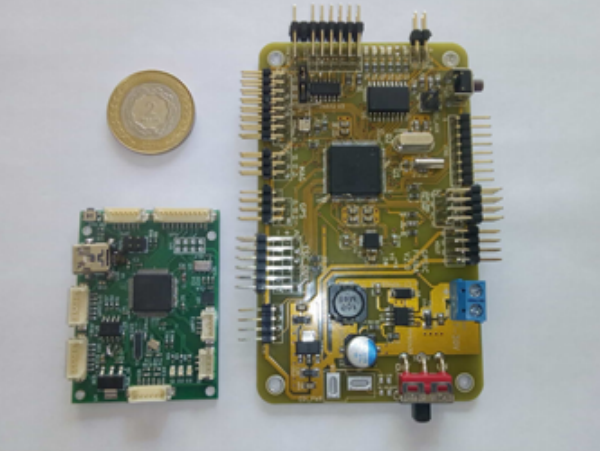
\includegraphics[width=0.5\textwidth]{choriboards_anteriores.png}
%    \caption{}    
%\end{figure}

%Hablar un poco de los sensores y componentes que tenían las computadoras anteriores y cómo fueron evolucionando.

%%%%%%%%%%%%%%%%%%%%%%%%%%%%%%%%%%%%%%%
%Todas las computadoras cuentan con un sistema de navegación inercial INS. Explicar brevemente qué es y por qué es importante.

% Tesis de Claudio:
%Los sensores inerciales son un tipo de sensores que permiten medir fuerzas específicas y velocidades de giro, mediante el uso de acelerómetros y giróscopos, generalmente ordenados en grupos de tres para medir dichos valores sobre cada eje de la terna. Este tipo de sensores permiten obtener datos a altas frecuencias, y se verá que cumplen un papel vital en la determinación de los ángulos de navegación.
%
%Dentro de los instrumentos de medición, pueden identificarse dos grupos. Por un lado, están los sensores cuyos datos son de gran importancia para la estabilidad del UAV, que son los que proveen las mediciones de los acelerómetros y giróscopos. Como ya fue mencionado, éste tipo de datos necesitan una alta frecuencia de actualización, y la demora en adquirir los datos debe ser la mínima posible.

% Tesis de Tournour
%Uno de los sistemas de navegación utilizados son los sistemas inerciales (INS por sus siglas en inglés). Estos sistemas resuelven las ecuaciones inerciales de la navegación integrando la información de los sensores. Los sensores inerciales utilizados comúnmente son los acelerómetros, para medir aceleraciones, y los giróscopos, para medir velocidades angulares. Existe una amplia variedad de sensores inerciales, pero dados los requerimientos de la aplicación en Vehículo Aéreo No Tripulado (VANT)s los que mejor se adaptan son los sensores microelectromecánicos o MEMS (del inglés Microelectromechanical MEMS Systems). Estos sensores permiten medir una amplia variedad de magnitudes, con las ventajas de su bajo costo, bajo peso, su pequeño tamaño, y su amplio ancho de banda (1kHz aprox.). En la Figura 1.2 se puede observar dos de estos sensores.

Un sistema de navegación permite realizar estimaciones de la pose del vehículo, es decir de la posición y orientación. En la figura \ref{fig:angles_drone} se muestra un UAV con una terna solidaria a este. La forma de indicar la orientación del vehículo es a través de los ángulos denominados \textit{yaw}, \textit{pitch} y \textit{roll}. Estos expresan las rotaciones entre la terna solidaria al vehículo en su posición actual, y una terna inercial, fija en el espacio.

\begin{figure}[H]
    \centering
    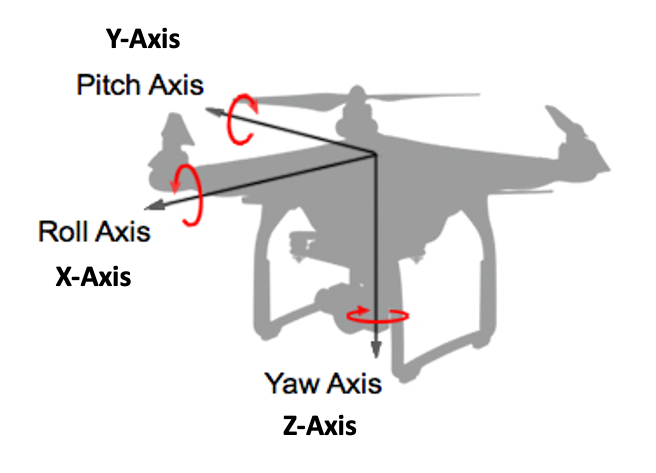
\includegraphics[width=0.5\textwidth]{angles_drone.png}
    \caption{Se utiliza una terna solidaria al vehículo para conocer su orientación en el espacio. Los ángulos \textit{yaw}, \textit{pitch} y \textit{roll} indican rotaciones respecto de una terna inercial.}
    \label{fig:angles_drone}    
\end{figure}

El principal sistema utilizado en UAVs es el sistema de navegación inercial (INS). Este consiste en realizar estimaciones de posición y orientación a partir de integrar en el tiempo mediciones de aceleración y velocidad de rotación del vehículo. Por ejemplo, podrían conocerse los ángulos de la figura \ref{fig:angles_drone} a partir de mediciones de velocidad angular. Estos sistemas no solo se utilizan en UAV sino que también en vehículos tripulados y aviones comerciales.

El hecho de integrar las mediciones de velocidad y aceleración en el tiempo, trae consigo que cualquier error de los acelerómetros y los giróscopos decante en errores de posición y de orientación que crecerán con el paso del tiempo a un ritmo acelerado. Típicamente esto se corrige utilizando otro sistema de navegación auxiliar (como por ejemplo a través de GPS) junto con un filtro de Kalman o un sistema equivalente. %En la figura \ref{fig:kalman} se muestra un diagrama en bloques que relaciona al sistema inercial con el sistema auxiliar a través del filtro de Kalman para corregir las salidas del sistema de navegación inercial.

% \begin{figure}[H]
%     \centering
%     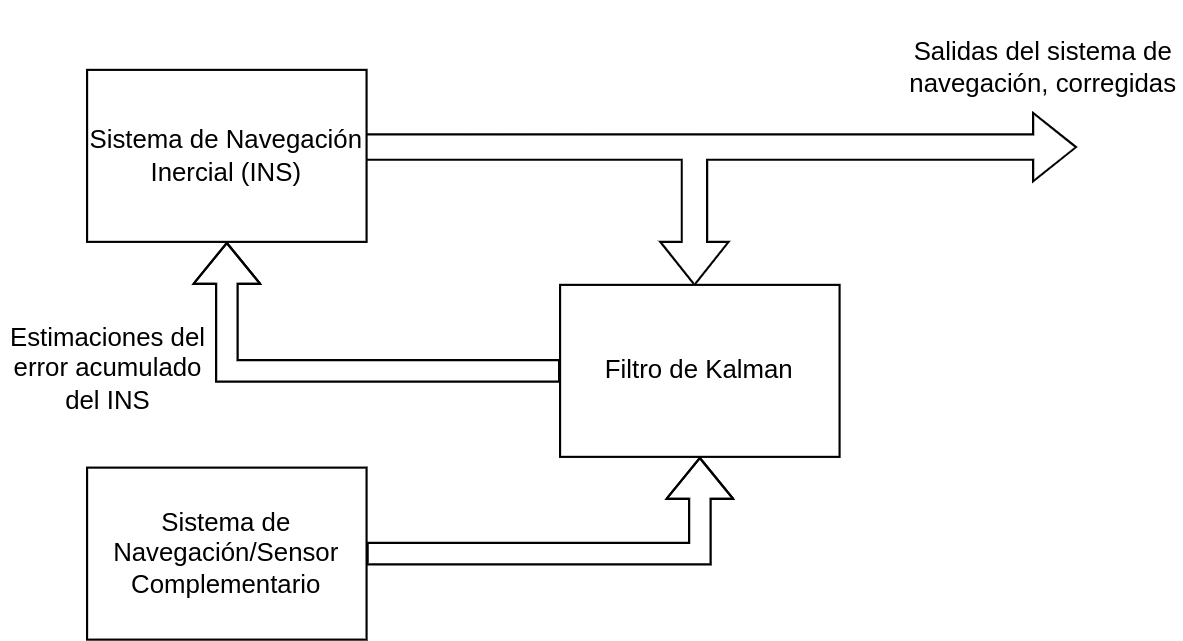
\includegraphics[width=0.8\textwidth]{kalman.png}
%     \caption{Diagrama en bloques del INS junto con un sistema de navegación auxiliar de GPS. Ambos se complementan a partir del filtro de Kalman.}
%     \label{fig:kalman}
% \end{figure}

Para obtener las mediciones de aceleración y velocidad angular en la computadora de vuelo, se utilizará una Unidad de Medición Inercial (IMU). Esta comprende acelerómetros y giróscopos triaxiales, los cuales se denominan sensores inerciales. La IMU ofrece una alta tasa de adquisición de datos, en el orden de las decenas de kHz. Esto es de gran importancia para mantener la estabilidad del vehículo, ya que utilizando acelerómetros y giróscopos es posible estimar los ángulos de \textit{pitch} y \textit{roll} del vehículo. 

%%%%%%%%%%%%%%%%%%%%%%%%%%%%%%%%%%%%%%%

% El sistema de navegación inercial requiere que se resuelvan muchas ecuaciones. Para eso se incorpora una unidad de procesamiento:
%
% Por qué se usa un microcontrolador COTS?
% - Bajo costo
% - Tamaño reducido.
% - La gran cantidad de interfaces que integran.
% - Necesidad de una respuesta con determinismo temporal.

Para realizar todos los cálculos involucrados en el INS, se utiliza una unidad de procesamiento. Todas las tareas involucradas en navegación y control de vuelo son ejecutadas de forma periódica por la computadora de vuelo. Se requiere asegurar un determinismo temporal en la ejecución de las tareas, del orden de los milisegundos o decenas de milisegundos. La unidad de procesamiento que mejor se ajusta a las necesidades de este trabajo es un microcontrolador de 32 bits, siendo el principal motivo la gran variedad que pueden encontrarse en el mercado, los cuales ofrecen una muy buena performance por un bajo costo. La gran capacidad de cómputo que ofrecen permite que este además puede realizar otras tareas más, como encargarse de la tolerancia a fallas, el almacenamiento de datos y otras tareas relacionadas a la misión del vehículo.

Otro factor importante es el gran nivel de integración que ofrecen, incorporando gran variedad y cantidad de periféricos e interfaces de comunicación. Esto favorece la posibilidad de obtener un diseño de dimensiones pequeñas.

Algunas de las funcionalidades secundarias que se implementan son el control de LEDs indicadores de propósito general y la capacidad de almacenamiento de datos en una memoria externa, tanto de sensores como de datos pertinentes a la misión del vehículo. Además, de manera de ampliar las capacidades, se incorpora una gran variedad de conectores que facilitan la comunicación con dispositivos y sensores externos. Esto le da una gran versatilidad, en el sentido de que permite su utilización en distintas aplicaciones de UAVs y vehículos no tripulados en general.

%Se aprovechan las distintas interfaces que ofrecen estos componentes para 

%Para realizar los cálculos se integra una unidad de procesamiento. Teniendo en cuenta versiones anteriores de la computadora de vuelo, se utiliza un microcontrolador ARM. Además de la retrocompatibilidad con versiones anteriores. Esta también será la unidad central de la placa, encargándose de las tareas de tolerancia a fallas, almacenamiento de datos y otras tareas relacionadas a la misión del vehículo.

%Es un sistema de tiempo real, se requiere determinismo en el cálculo.

%Necesidad de tener un tamaño reducido.

%%%%%%%%%%%%%%%%%%%%%%%%%%%%%%%%%%%%%%%

%no está pensada para usarse en un único tipo de vehículo, sino que puede utilizarse en vehículos con distintas arquitecturas. Esto implica la necesidad de interfaces varias para conectar módulos y sensores.

%%%%%%%%%%%%%%%%%%%%%%%%%%%%%%%%%%%%%%%

%La computadora de vuelo debe tener cierta versatilidad para implementar distintas arquitecturas redundantes para la implementación de la tolerancia a fallas.

%%%%%%%%%%%%%%%%%%%%%%%%%%%%%%%%%%%%%%%

%Otras de las funcionalidades son el control de LEDs indicadores de propósito general y la capacidad de almacenamiento de datos, tanto de sensores como de datos pertinentes a la misión del vehículo. A lo largo de esta sección se irán mencionando otras funcionalidades secundarias.

% El modelo de este componente se ha ido actualizando con las distintas versiones. Con el pasar de los años, los modelos de las primeras versiones se han ido disconinuando, dando paso a nuevos sensores que ofrecen mejores prestaciones, como por ejemplo en cuanto a ruido, offset, sensibilidad, entre otros.

% Los componentes comunes son la IMU, el uso de un microcontrolador cortex MX, salidas PWM para control de motores, tienen muchos puertos auxiliares para conectar varias cosas externas. 

% La placa desarrollada en este trabajo es una nueva versión de la computadora de vuelo. Se busca tal cosa...

%Mencionar que ya existían otras placas previas del LAR y que ahora se está haciendo una versión nueva.

%La computadora debe ser versátil, en el sentido de que no está pensada para usarse en un único tipo de vehículo, sino que puede utilizarse en vehículos con distintas arquitecturas.

%Actualización de los componentes y sensores para mejorar el rendimiento y reemplazar dispositivos obsoletos y/o discontinuados.

%Retrocompatibilidad con módulos de firmware desarrollados para la versión anterior. También retrocompatibilidad en los conectores, de manera de conectar módulos que se utilizaron en la versión anterior.

%Electrical transmission of signals and commands is a key element in a FBW system. Modern systems use a serial digital data transmission system with time division multiplexing. The signals can then be transmitted along a network or highway comprising two wires only, as only one set of data is being transmitted at any particular time. Figure 4.2 shows how a digital flight control system is interconnected using a digital data bus.

% Entrada de programación
% Debugger
% Botón reset
% IMU (SPI)
% Barómetro Integrado (I2C)
% Magnetómetro Externo (I2C)
% GPS externo (UART)
% Salidas PWM para motores + servos para otra cosa
% DSM para Spektrum
% PPM para radios en general
% Conector fuente externa tipo pixhawk
% microSD
% LEDs Integrados para indicadores
% UARTs adicionales para conectar cosas externas
% I2C adicional
% SPI adicionales
% salidas de 5V y 3V3
% switches para distintas funcionalidades

%%%%%%%%%%%%%%%%%%%%%%%%%%%%%%%%%%%%%%%

\subsection{Criterios Generales Para la Selección de Componentes}

% Acá no se dan justificaciones de algún circuito en particular, sino que se dan justificaciones que aplican a todos los bloques. Por ejemplo, el tema del AEC-Q100 y los pedidos del laboratorio, como los pines dupont, etc.

Para el diseño y construcción de la computadora de vuelo, se tuvieron en cuenta algunos criterios comunes a todos los componentes. Estos se mencionan a continuación.

% de cada circuito, se tuvieron en cuenta distintas necesidades particulares para cada uno de ellos. A su vez, hay ciertos criterios y que son comunes a todos los circuitos. Estos se mencionan a continuación.

\subsubsection{Uso de Componentes de Grado Automotriz}

Una de las premisas de cualquier trabajo de desarrollo de electrónica, consiste en que este sea de un bajo costo. Gracias al avance de la tecnología, en los últimos años se han ido abaratando los costos de fabricación de chips y componentes electrónicos. Haciendo una búsqueda rápida en sitios web de distintos proveedores de componentes puede encontrarse que existe una gran variedad de estos, como sensores y microcontroladores, a precios razonables.

En el caso particular de sistemas críticos, el aspecto más importante y fundamental es el de la confiabilidad. Generalmente este requerimiento impacta en el costo del desarrollo, ya que la confiabilidad suele traer consigo altos costos de fabricación. Por ejemplo, % AGREGAR EJEMPLOS DE COMPONENTES USADOS EN AVIONES.

% ENTONCES, SE QUIERE HACER ALGO SAFETY-CRITICAL PERO DE BAJO COSTE. ==> MENCIONAR LA OFERTA DE COMPONENTES AUTOMOTRIZ Y HABLAR DE AEC-Q100

\textbf{{\color{red} COMPLETAR}}

\subsubsection{Longevidad}

%Quizás uno de los criterios más importantes es el de la longevidad de los componentes. En un desarrollo de electrónica se seleccionan componentes de muchos fabricantes. 

Para el desarrollo de la placa se buscaron componentes para los cuales el fabricante garantice la longevidad antes de entrar en fin de vida útil. En el eventual caso de que un componente deje de ser fabricado, a futuro esto impactará en el diseño, ya que será necesario buscar un reemplazo del mismo, para poder fabricar nuevas unidades. Algunas veces esto es directo, ya que algunos fabricantes ofrecen compatibilidad en los terminales de componentes de mismas funcionalidades. Sin embargo en otros casos, esto puede traer consecuencias como la necesidad de modificar el diseño original, además de volver a realizar pruebas del circuito, utilizando el nuevo componente. En el caso de que se trate de un sensor, incluso puede requerir la modificación del driver utilizado para interactuar con este.

Para la computadora de vuelo de este trabajo, se buscó tener una longevidad de 10 años.

%\textbf{{\color{red} COMPLETAR}}

\subsubsection{Requerimientos de Conectores}

La computadora de vuelo cuenta con una serie de conectores que permiten el agregado de módulos externos. Algunos de esos conectores fueron seleccionados por una necesidad de tener compatibilidad con distintos módulos que son comúnmente utilizados con otras computadoras de vuelo. Estos serán mencionados en las secciones correspondientes.

\subsection{Circuitos y Componentes Seleccionados}

A continuación se describe cada una de las partes del circuito que conforman a la computadora de vuelo. Además de los criterios generales ya mencionados, se mencionan los criterios particulares tenidos en cuenta para cada parte del circuito.

%\subsection{Circuitos Implementados}
\subsubsection{Microcontrolador}

% Acá sí, va una subsubsection por cada bloque, por ejemplo microcontrolador, IMU, Barómetro, bus CAN, Tarjeta Micro SD, Interfaz USB, etc.

%\subsubsection{Microcontrolador}
%\subsubsection{Selección del Componente}

En la versión anterior de la computadora de vuelo, se utilizó un microcontrolador del fabricante ST, en particular el modelo STM32F722. Este cuenta con un procesador ARM Cortex-M7, que puede utilizarse con una frecuencia máxima de 216 MHz. Cuenta con unidad de punto flotante integrada, además de una memoria flash con 512 KB y una memoria RAM de 256 KB.

A todas las funcionalidades de la computadora de vuelo, en este trabajo se le suman los aspectos relacionados a la tolerancia a fallas. A su vez, se tiene la necesidad de integrar otras funcionalidades que llevan consigo una gran carga computacional. Estas pueden ser propias de la aplicación del vehículo o bien relacionadas a mejorar los algoritmos de navegación y control. Para la versión desarrollada en este trabajo, se buscó actualizar el microcontrolador a uno con mayor rendimiento, sin perder de vista la necesidad de mantener un costo reducido.

Se buscó un microcontrolador del mismo fabricante ST, de manera de tener retrocompatibilidad en el desarrollo del firmware con la versión anterior. De esta forma, muchos de los módulos de firmware que ya se encuentran desarrollados pueden reutilizarse en esta nueva versión. Con estos requerimientos, se analizaron las distintas ofertas del mercado. Además de los aspectos mencionados, se tuvieron en cuenta los periféricos presentes en cada modelo, junto con las capacidades de memorias flash y RAM. Se buscó mantener las capacidades de estas memorias en valores similares a las de la versión anterior de la computadora de vuelo.

Como primera opción surgió la posibilidad de seleccionar alguno de los microcontroladores de la serie STM32H7. Estos cuentan con procesadores ARM Cotex-M7, y pueden llegar a velocidades entre 400 MHz y 550 MHz \cite{AN5293}, es decir, pueden llegar hasta a duplicar la performance respecto de la versión anterior de la computadora de vuelo. En la tabla \ref{tab:comparacion_MCUs} se muestran distintos modelos que fueron considerados durante la selección del microcontrolador.

\begin{table}[H]
    \centering
    \begin{tabular}{|c||c|c|c|c|c|c|}
        \hline
                        & STM32F722 & STM32H723ZG & STM32H743 & STM32H753 & STM32H735ZG \\
        \hline
        Flash [kB] & 512 & 1024 & \cellcolor{green!25}1024/2048 & \cellcolor{green!25}2048 & 1024\\
        \hline
        SRAM [kB]  & 256 & 564 & \cellcolor{green!25}1024 & \cellcolor{green!25}1024 & 564\\
        \hline
        Freq [MHz] & 216 & \cellcolor{green!25}550 & 480 & 480 & \cellcolor{green!25}550\\
        \hline
        UART & 4 & \cellcolor{green!25}6 & 4 & \cellcolor{green!25}6 & \cellcolor{green!25}6\\
        \hline
        USART & 4 & \cellcolor{green!25}5 & 4 & \cellcolor{green!25}5 & \cellcolor{green!25}5\\
        \hline
        SPI & 5 & \cellcolor{green!25}6 & \cellcolor{green!25}5/6 & \cellcolor{green!25}6 & \cellcolor{green!25}6\\
        \hline
        I2C & 3 & \cellcolor{green!25}5 & 4 & 4 & \cellcolor{green!25}5\\
        \hline
        CAN & 1 & \cellcolor{green!25}3 & 2 & \cellcolor{green!25}3 & \cellcolor{green!25}3\\
        \hline
        ADC & 3x12b, 24ch & \makecell{2x16b, 22 ch; \\ 1x12b, 12 ch} & \cellcolor{green!25}\makecell{3x16b, \\ 16/28/32ch} & \makecell{1x12b, 12ch \\ 2x16b, 18ch} & \makecell{1x12b, 12ch \\ 2x16b, 16ch}\\
        \hline
        Timers & \makecell{18: 16b x 16, \\ 32b x 2} & \cellcolor{green!25}\makecell{21: 16b x 17, \\ 32b x 4} & \makecell{14: 16b x 12, \\ 32b x 2} & \cellcolor{green!25}\makecell{21: 16b x 17, \\ 32b x 4} &\cellcolor{green!25} \makecell{21: 16b x 17, \\ 32b x 4}\\
        \hline
        SDMMC & \cellcolor{green!25}2 & \cellcolor{green!25}2 & \cellcolor{green!25}2 & \cellcolor{green!25}2 & \cellcolor{green!25}2\\
        \hline
        longevidad & \cellcolor{green!25}01/2033 & \cellcolor{green!25}01/2033 & \cellcolor{green!25}01/2033 & \cellcolor{green!25}01/2033 & \cellcolor{green!25}01/2033\\
        \hline
        AEC-Q100 & No & No & No & No & No\\
        \hline       
    \end{tabular}
    \caption{Se muestra la comparación de las distintas alternativas que fueron tenidas en cuenta para la selección del mircocontrolador. En verde se destaca el componente que tiene las mejores características para cada fila. El modelo STM32F722 corresponde al modelo utilizado en la versión anterior de la computadora de vuelo.}
    \label{tab:comparacion_MCUs}
\end{table}

Todos los microcontroladores de la serie STM32H7 presentan mejoras en cuanto a frecuencia de operación, memoria flash y RAM. Sumado a esto, la gran mayoría de estos microcontroladores se encuentran dentro del programa \textit{Longevity Commitment} \cite{longevity_ST}. El fabricante ST se compromete a mantener la producción de los componentes que se encuentren dentro de este programa durante un período determinado. Todos los microcontroladores de la tabla \ref{tab:comparacion_MCUs} tienen un periódo de fabricación de 10 años asegurado por ST, finalizando en 01/2033. Este aspecto es de especial interés teniendo en cuenta la posible necesidad futura de fabricar nuevas placas de la computadora de vuelo.

\textbf{{\color{red} COMPLETAR POR QUÉ NO SE ELEIGIÓ UNO AEC-Q100, QUE ES PORQUE NO HABÍA CORTEX M7 DE ST QUE SEA AEC-Q100}}

%\textbf{{\color{red} COMPLETAR LA JUSTIFICACIÓN DE QUE SE ELIGIÓ UN MICROCONTROLADOR DIFERENTE DEBIDO A LA CRISIS Y FALTANTE DE CHIPS}}

% Acá lo importante es decir que se quería elegir un controlador más potente que la choriboard III, algún STM32H7. Mencionar por qué STM32, que es porque ellos vienen trabajando con esos microcontroladores. Luego explicar que debido al faltante y la crisis, se tuvo que elegir otro controlador. También, mencionar que el que se eligió tiene 10 años de garantía de fabricación, lo que favorece la longevidad.

A pesar del análisis y de las comparaciones entre microcontroladores de la serie STM32H7, la selección del microcontrolador se vio limitada por la disponibilidad de componentes encontrada durante el período de desarrollo del circuito.

\textbf{{\color{red} SE PUEDE SIMPLEMENTE MENCIONAR LA CRISIS DE CHIPS COMO CAUSA DE LA FALTA DE DISPONIBILIDAD.}}

El microcontrolador seleccionado fue el STM32F746ZG. Este cuenta con un procesador ARM-Cortex M7, 1024 kB de memoria flash y 320 kB de memoria SRAM. Un aspecto relevante de este microcontrolador es que cuenta con 2 interfaces para uso de un bus denominado Controller Area Network (CAN), el cual se utilizará para establecer las comunicaciones relevantes a los algoritmos de tolerancia a fallas. La posibilidad de contar con dos de estas interfaces permite implementar un sistema donde este bus no sea un punto singular de falla.

Suamdo a las prestaciones, este micocontrolador cuenta con un encapsulado LQFP de 144 terminales, lo que permite realizar muchas conexiones con sensores y componentes a través de distintas interfaces comunes, como SPI, I2C, además de terminales GPIO comunes para interrupciones y manejo de otros módulos.

\textbf{{\color{red} SE PUEDE EXPLICAR LA SELECCIÓN DE LOS CRISTALES Y EL USO DE LOS CAPACIOTRES DE DESACOPLE, SIGUIENDO LA APP NOTE DE ST.}}

% Mencionar cómo se asignaron los distintos timers para su uso en la aplicación.


% Mencionar cómo se asignaron las interrupciones externas de gpios.

% Acá también hay que mencioanr todos los cálculos y justificaciones para la selección del cristal, tanto de 12 MHz como el de 32 kHz. Poner todo lo que tengo, esta sección tiene muchísimo para mostrar.

%\textbf{{\color{red} COMPLETAR}}

%\subsection{Otros Circuitos Implementados}

%\subsubsection{Sensor IMU}

%\subsubsection{Requerimientos del Componente}

%\textbf{{\color{red} COMPLETAR}}

% acá van todos los capacitores de desacople, etc

%\subsubsection{Cristal Externo}

%\textbf{{\color{red} COMPLETAR}}

%\subsubsection{Cristal para RTC}

%\textbf{{\color{red} COMPLETAR}}

\subsubsection{Sensor IMU}

La unidad de medición inercial, IMU por sus siglas en inglés, es el sensor principal utilizado por la computadora de vuelo. Este consiste en un circuito integrado que contiene una serie de sensores inerciales, en particular acelerómetros y giróscopos triaxiales. Los acelerómetros se utilizan para realizar mediciones de aceleración lineal y los giróscopos para medir velocidad angular. A partir de estas mediciones, se pueden aplicar distintos algoritmos de procesamiento para obtener una estimación de la posición y orientación del vehículo. Las mediciones de aceleración lineal y de velocidad angular que entrega la IMU son referidas a una terna solidaria al componente, como se muestra en la figura \ref{fig:IMU_ejes}.

\begin{figure}[H]
    \centering
    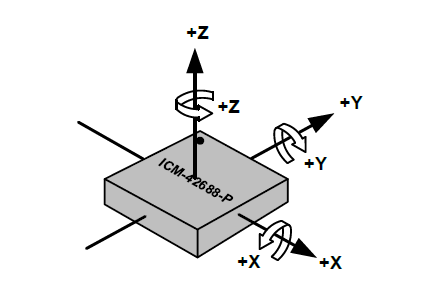
\includegraphics[width=0.4\textwidth]{img/IMU_ejes.png}
    \caption{Todas las mediciones que entrega el sensor son realtivas a una terna solidaria a este. La imagen se extrajo de \cite{ICM42688pDatasheet}.}
    \label{fig:IMU_ejes}
\end{figure}

\textbf{{\color{red} REEMPLAZAR LO QUE SIGUE POR UNA SIMPLE MENCIÓN DE SENSORES MEMS, DESDE ACÁ:}}

Los acelerómetros y giróscopos de la IMU utilizada en este trabajo, se construyen utilizando la tecnología MEMS: \textit{Microelectromechanical Systems}. Utilizando técnicas de fabricación de circuitos integrados, se construyen los acelerómetros y giróscopos, integrando en el silicio partes que son móviles. En la figura \ref{fig:MEMS_acelerometro}, se muestra una imagen tomada con un microscopio electrónico de un acelerómetro MEMS. Lo que se observa en este caso, es que en el mismo silicio se integra una masa llamada \textit{proof-mass}, la cual se encuentra sujeta al sustrato a través de dos resortes.

\begin{figure}[H]
    \centering
    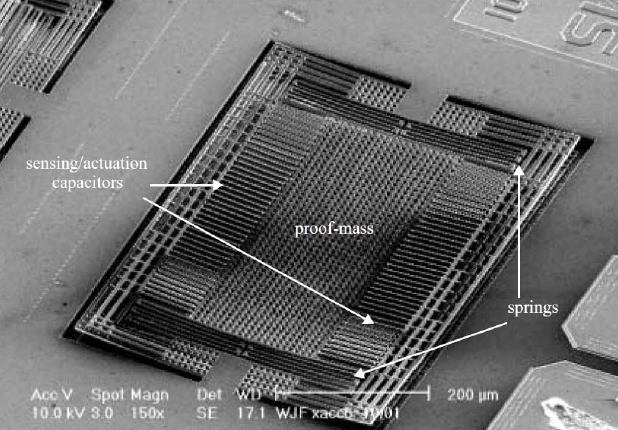
\includegraphics[width=0.6\textwidth]{img/MEMS_acelerometro.png}
    \caption{Fotografía tomada de un acelerómetro construido con tecnología MEMS. La imagen se extrajo de \cite{zhang2010sensing}. }
    \label{fig:MEMS_acelerometro}    
\end{figure}

Una aceleración sobre el componente genera que la masa del acelerómetro se mueva. Estos desplazamientos producen una variación en la capacidad existente entre el sustrato y la masa, lo que lleva a una variación de la tensión entre ambos. Esta diferencia de potencial variable es medida por un circuito dentro del chip, y que luego se utiliza para generar las mediciones de aceleración.\\

El acelerómetro puede modelarse de manera simple, como un sistema mecánico con una masa, un resorte y un amortiguador \cite{zhang2010sensing}, como se muestra en la figura \ref{fig:acelerometro_modelo}.

\begin{figure}[H]
    \centering
    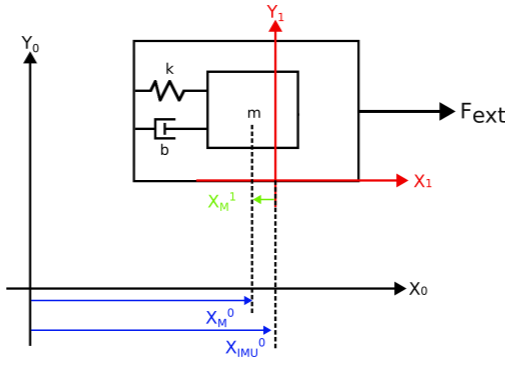
\includegraphics[width=0.5\textwidth]{img/acelerometro_modelo.png}
    \caption{Sistema mecánico simplificado del acelerómetro.}
    \label{fig:acelerometro_modelo}    
\end{figure}

La terna 0 corresponde a una terna inercial, mientras que la terna 1 es no inercial, solidaria al movimiento del acelerómetro. Cabe aclarar que tal como se mencionó, la masa se encuentra sujeta al sustrato solamente a través del resorte. El elemento amortiguador representa pérdidas de energía, causadas por rozamiento con el aire o de la propia estructura electromecánica. Se puede resolver el sistema mecánico, tomando como coordenadas generalizadas $q_1 = X_{IMU}^0$ y $q_2 = X_M^1$. Sin considerar efectos de la gravedad, se llega a la ecuación \eqref{eq:acelerometro_segundo_orden}. Este es un sistema de segundo orden, donde la entrada es la aceleración del acelerómetro y la salida es el desplazamiento de la masa respecto de la terna solidaria al acelerómetro. 

\begin{equation}
    \ddot{X_M^1} + \frac{b}{m} \dot{X_M^1} + \frac{k}{m} X_M^1 = -\ddot{X_{IMU}^0}
    \label{eq:acelerometro_segundo_orden}
\end{equation}

Como resultado interesante, se observa que el sistema es de segundo orden, típicamente con respuesta sub-amortiguada. Algunos fabricantes de estos sensores indican en sus hojas de datos, un valor de frecuencia de resonancia. Este valor resulta de interés ya que si se excita al sensor con frecuencias cercanas a la resonancia, dejará de funcionar como dispositivo para medir la aceleración lineal. Por otro lado, a muy bajas frecuencias se puede despreciar la velocidad de la masa y luego se obtiene una relación directa entre la aceleración del acelerómetro y el desplazamiento de la masa, ecuación \eqref{eq:relacion_aceleracion_despalzamiento}.

\begin{subequations}
	\begin{align}
        \ddot{X_M^1} &\approx 0\\
        \dot{X_M^1} &\approx 0\\
        \frac{k}{m} X_M^1 &\approx -\ddot{X_{IMU}^0}
	\end{align}
    \label{eq:relacion_aceleracion_despalzamiento}
\end{subequations}

El desplazamiento de la masa produce una variación de la capacidad entre esta y el sustrato. Esta capacidad es utilizada para medir una varaición de tensión \cite{zhang2010sensing}. El circuito medido puede modelarse como en la figura \ref{fig:acelerometro_sensado_capacitivo}.

\begin{figure}[H]
    \centering
    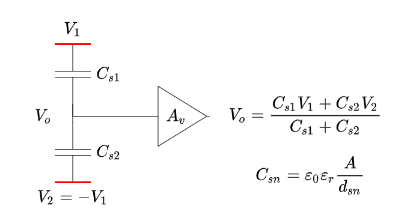
\includegraphics[width=0.5\textwidth]{img/acelerometro_sensado_capacitivo.png}
    \caption{Circuito equivalente que mide el desplazamiento de la masa. Las tensiones $V1$ y $V2$ representan señales de tensión aplicadas por un circuito externo. El movimiento de la masa modifica la capcidad y por ende la tensión medida.}
    \label{fig:acelerometro_sensado_capacitivo}    
\end{figure}

Se puede resolver este circuito y llegar a que existe una relación lineal entre la tensión $Vo$ y el desplazamiento de la masa $\Delta d$, ecuación \eqref{eq:tension_salida_acelerometro}. En \cite{zhang2010sensing} puede encontrarse la demostración completa. En la ecuación, $d_0$ representa la separación de reposo entre el sensor y el sustrato y $\Delta d$ la variación de la separación.

\begin{equation}
    V_{o} = \frac{\Delta d}{d_0} V_1
    \label{eq:tension_salida_acelerometro}
\end{equation}

\textbf{{\color{red} HASTA ACÁ}}

%\textbf{{\color{red} COMPLETAR UN ANÁLISIS SIMILAR PARA EL GIRÓSCOPO}}

Se hizo una búsqueda de las distintas alternativas existentes para este tipo de sensores. A partir de leer las hojas de datos de distintos fabricantes, se encontró que los parámetros típicamente especificados, tanto para los acelerómetros como para los giróscopos, son los siguientes:

\begin{itemize}
    \item \textit{Full-scale range}
    \item \textit{Sensitivity}
    \item \textit{Scale factor error}
    \item \textit{Scale factor error vs temp}
    \item \textit{Offset}
    \item \textit{Offset vs temp}
    \item \textit{Offset vs time}
    \item \textit{Noise}
\end{itemize}

El primero de ellos, el \textit{Full-scale range} es el rango de medición del sensor. Para los acelerómetros se suele especificar en un rango de $\pm n \times g$, donde $n$ es algún entero y $g$ representa la aceleración de la gravedad. Para los giróscopos, se especifica como $\pm n \times dps$, donde $dps$ significa \textit{degrees-per-second}.\\

El parámetro \textit{Sensitivity} hace referencia a la resolución. En algunas hojas de datos este parámetro puede encontrarse con unidades de $LSB/g$ para los acelerómetros y en $LSB/dps$ para los giróscopos. Este valor puede resultar confuso de entender, ya que lo que informa es la cantidad de bits por $g$ o la cantidad de bits por $dps$. En la figura \ref{fig:ICM_42688_datasheet} se muestra una captura de la hoja de datos del sensor seleccionado, el ICM42688p. 

\begin{figure}[H]
    \centering
    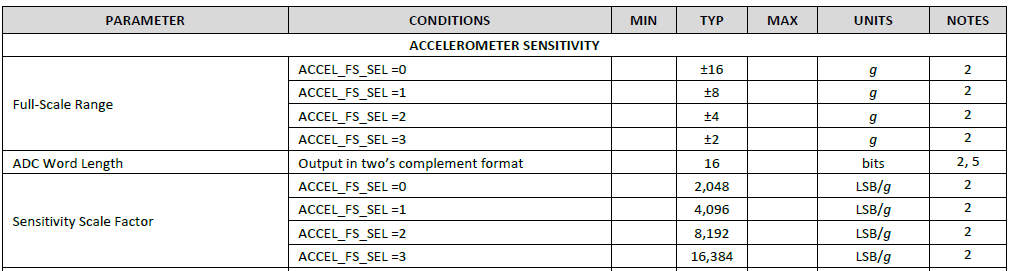
\includegraphics[width=\textwidth]{img/ICM_42688_datasheet.png}
    \caption{Extracto de la hoja de datos del sensor ICM42688p. Se muestra parte de las especificaciones para los acelerómetros.}
    \label{fig:ICM_42688_datasheet}    
\end{figure}

La imagen muestra que el sensor permite seleccionar distintos rangos de escala para las mediciones del acelerómetro. Por ejemplo, si se selecciona el rango $\pm 2g$, la hoja de datos especifica una resolución de $16384 \ LSB/g$. Una mejor forma de entender este parámetro sería si se considera la inversa, es decir, la resolución del ADC. En este caso sería de $61.04 \ 10^{-6} \ g$. Luego para un rango de $\pm 4g$ la resolución es de $8192 \ LSB/g$, es decir, $122.07 \ 10^{-6} \ g$. Este valor es el doble del anterior y tiene sentido dado que se está midiendo un rango mayor de aceleraciones utilizando la misma cantidad de bits, en este caso 16 según lo especificado en la hoja de datos.\\

Para entender los parámetros, \textit{scale factor error}, \textit{offset} y \textit{noise} se plantea un modelo sencillo de medición, tanto para acelerómetros como para giróscopos \cite{borodacz2022review}. Este se presenta en la ecuación \eqref{eq:medicion_vs_real}, donde $S$ es el \textit{scale factor error}, $\omega_b(t)$ es el \textit{offset} el cual es variable con el tiempo, $\eta \sim \mathcal{N}(0,\sigma^2)$, $\omega_m$ es el valor medido y $\omega$ sería la velocidad angular verdadera para el giróscopo.

\begin{equation}
    \omega_m = (1+S)\omega + \omega_b (t) + \eta
    \label{eq:medicion_vs_real}
\end{equation}

A su vez, en las hojas de datos se especifica la dependencia de estos parámetros con el tiempo y con la temperatura, como es el caso del \textit{scale factor error}.\\

Para tener un criterio de selección del sensor IMU, se siguió el análisis planteado en \cite{borodacz2022review}. Este paper presenta un análisis de los parámetros de los acelerómetros y grióscopos y su impacto en las estimaciones de posición en sistemas de navegación inercial (INS). En este se concluye que los parámetros más importantes para la selección del sensor son:

\begin{itemize}
    \item Estabilidad del offset de los acelerómetros (Offset vs time).
    \item Estabilidad del offset de los giróscopos (Offset vs time).
    \item Ruido de los giróscopos (Noise).
    \item Error de escala del giróscopo (Scale factor error).
\end{itemize}

Se buscaron modelos de IMUs de distintos fabricantes, para comparar características. Existe una gran cantidad de fabricantes y de componentes para seleccionar. Se buscaron componentes que sean accesibles y que no tengan un costo muy elevado. Existen IMUs de una excelente calidad, pero que tienen precios que no están al alcance (cientos o miles de dólares). Con este criterio, se realizó una comparación entre distintos modelos de sensores. En la tabla \ref{tab:comparacion_IMUs} se muestra una comparación de los distintos sensores considerados. Sumado a esto, se tuvo en consideración otro aspecto que fue mencionado anteriormente, la longevidad del componente.

\begin{table}[H]
    \centering
    \begin{tabular}{|c||c|c|c|c|c|}
        \hline
                        & ICM42688 & LSM6DSR & IIM-42652 & BMI088 & ASM330LHHX\\
        \hline
        $b_{accel}(t)$ & N/A      & N/A     & N/A       & N/A    & \cellcolor{green!25}40 $\mu$ g\\
        $b_{gyro}(t)$   & N/A      & N/A     & N/A       & \cellcolor{green!25}2°/h    & 3°/h\\
        $\eta_{gyro}$   & \cellcolor{green!25}$2.8 mdps/\sqrt{Hz}$ & $5 mdps/\sqrt{Hz}$ & $3.8 mdps/\sqrt{Hz}$ & $14 mdps/\sqrt{Hz}$ & $5 - 12 mdps/\sqrt{Hz}$\\
        $S_{gyro}$ & \cellcolor{green!25}$0.5 \%$ & $1 \%$ & \cellcolor{green!25}$0.5 \%$ & $1 \%$ & $2 \%$\\
        \hline
        longevidad & N/A & N/A & 10 años, dic. 2020 & N/A & \cellcolor{green!25}15 años, mayo 2022\\
        AEC-Q100 & No & No & No & No & \cellcolor{green!25}Sí\\
        \hline       
    \end{tabular}
    \caption{Se muestra la comparación de las distintas alternativas que fueron tenidas en cuenta para la selección del sensor. En verde se destaca el componente que tiene las mejores características para cada parámetro.}
    \label{tab:comparacion_IMUs}
\end{table}

Lo primero que llama la atención es el hecho de que muchos de los sensores no especifican todos sus parámetros. Una sola de las alternativas consideradas tiene disponible toda la información en su hoja de datos. Esto dificulta mucho la selección de un componente. A priori, se seleccionó el sensor ASM330LHHX por el hecho de ser el único que ofrece toda la información en su hoja de datos, además de ser de grado automotriz y tener una longevidad garantizada de 15 años. Teniendo en cuenta aspectos de confiabilidad, resulta esencial el hecho de conocer los parámetros del sensor.

Durante la selección del sensor hubo otro aspecto importante que se tuvo en cuenta y es el hecho de la compatibilidad con el software desarrollado por el laboratorio, para computadoras de vuelo anteriores a la de este trabajo. La versión anterior contaba con un sensor IMU ICM20602, del fabricante TDK. El laboratorio cuenta con bibliotecas de código ya desarrolladas para este sensor. Este presentó excelentes resultados, lo que sienta un antecedente importante en la selección de componentes del mismo fabricante. En la tabla \ref{tab:comparacion_IMUs_TDK} se muestra una comparación entre el sensor anterior ICM20602 y el sensor seleccionado ICM42688.

\begin{table}[H]
    \centering
    \begin{tabular}{|r||c|c|}
        \hline
         & ICM20602 & ICM42688 \\
        \hline
        Año & 2016 & 2021\\
        \hline
        \multicolumn{3}{|c|}{Giróscopos}\\
        \hline
        Full Scale Range[dps] & $\pm 250/500/1000/2000$ & $\pm 15/31/62/125/250/500/1000/2000$\\
        Scale Factor Error[\%] & $1.0$ @ 25°C & $0.5$ @ 25°C\\
        Scale factor error vs temp[\%/°C] & $0.016$ @ -40°C - 85 °C & $0.005$ @ 0°C - 70 °C\\
        Offset[dps] & $\pm 1$ & $\pm 0.5$\\
        Offset vs temp[dps/°C] & $0.01$ & $0.005$\\
        Offset vs time[°/h] & N/A & N/A\\
        Noise[$mdps/\sqrt{Hz}$] & $4$ & $2.8$\\
        \hline
        \multicolumn{3}{|c|}{Acelerómetros}\\
        \hline
        Full Scale Range[g] & $\pm 2/4/8/16$ & $\pm 2/4/8/16 $\\
        Scale Factor Error[\%] & $1.0$ @ 25°C & $0.5$ @ 25°C\\
        Scale factor error vs temp[\%/°C] & $0.012$ @ -40°C - 85 °C & $0.005$\\
        Offset[mg] & $\pm 25$ & $\pm 20$\\
        Offset vs temp[mg/°C] & X,Y: $\pm 0.5$, Z: $\pm 1$ & $\pm 0.15$\\
        Offset vs time[$\mu$g/h] & N/A & N/A\\
        Noise[$\mu g/\sqrt{Hz}$] & $100$ & X,Y: $65$, Z: $70$\\        
        \hline       
    \end{tabular}
    \caption{Se muestra la comparación del sensor ICM20602 y el sensor seleccionado ICM42688.}
    \label{tab:comparacion_IMUs_TDK}
\end{table}

Para el diseño del circuito se siguieron las recomendaciones en la hoja de datos del componente. Este sugiere incluir una serie de capacitores de desacople en los terminales de alimentación del componente. Se elige utilizar una comunicación SPI en modo esclavo, donde el maestro es el microcontrolador, ya que pueden obtenerse mayores velocidades de comunicación, respecto de otros protocolos como I2C. De esta forma se logra una alta tasa de adquisición de datos de acelerómetros y giróscopos. Como ya fue mencionado, esto resulta clave para mantener la estabilidad del vehículo. El circuito completo puede encontrarse en el \nameref{appendix:circuito_esquematico}.

Dado que el sensor IMU es un esclavo en la comunicación SPI, este solo puede comunicarse con el microcontrolador cuando este último le permita hacerlo. Para que la IMU pueda informar el momento en el que se obtuvo una nueva lectura, el sensor dispone de una salida digital la cual puede conectarse a una entrada digital del microcontroldor. Cuando el microcontrolador detecta un cambio de nivel en esta entrada, el mismo procede a solicitar el dato a través de la comunicación SPI. En la figura \ref{fig:IMU_SPI} se muestra un esquema de la conexión entre el controlador y el sensor IMU.

\begin{figure}[H]
    \centering
    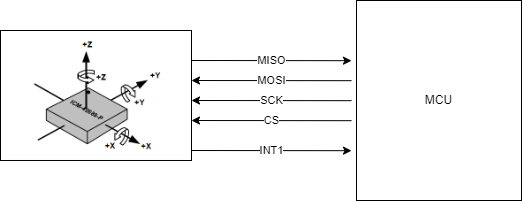
\includegraphics[width=0.8\textwidth]{img/IMU_SPI.png}
    \caption{Líneas de comunicación entre la IMU y el microcontrolador.}
    \label{fig:IMU_SPI}    
\end{figure}

\subsubsection{Barómetro}
%\subsection{Barómetro}

El barómetro se utiliza para obtener una estimación precisa de la altitud a la que está operando el UAV, a partir de mediciones de presión. Este es uno de los sensores complementarios al INS que se incorporan en la computadora de vuelo. Al igual que la IMU, el barómetro que se utiliza corresponde a un sensor de tecnología MEMS. En particular, los barómetros MEMS cuentan con un sistema capaz de medir la presión absoluta, es decir respecto al 0 de presión. Estos cuentan con una cavidad integrada dentro del chip que se encuentra (idealmente) a presión 0. %A través de un proceso llamado \textit{anodic bonding} \cite{baro_1}\cite{baro_2} se construye esta cavidad dentro del chip, la cual se encuentra sellada a una presión muy baja, en comparación con las presiones que se esperan medir utilizando el componente.
Para medir la presión, se coloca una membrana sobre la cavidad. En la figura \ref{fig:MEMS_barometro} se puede apreciar el efecto de la presión externa. 

\begin{figure}[H]
    \centering
    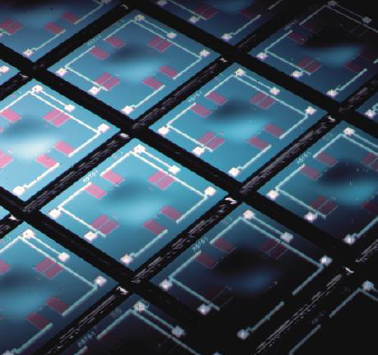
\includegraphics[width=0.4\textwidth]{img/MEMS_barometro.png}
    \caption{Sensores de presión sobre una oblea de silicio \cite{baro_1}.}
    \label{fig:MEMS_barometro}
\end{figure}

Sobre esta membrana se colocan resistores de efecto piezoresistivo en configuración puente de Wheatstone. El efecto de la presión genera compresiones y deformaciones en los resistores \cite{baro_3}, lo que se traduce en un desbalance del puente. A partir del sensado de la diferencia de potencial, se mide la presión aplicada sobre la membrana.


% En \eqref{eq:barometro_wheatstone} se despeja la relación entre la variación de tensión y la variación de la resistencia. Como se observa, la realación es proporcional.

% La deformación de la membrana genera tensión sobre estos, modificando su resistencia, de manera tal de que la presión comprime a dos de los resistores y estira a los otros dos \cite{baro_3}.


% Sobre las zonas de color violeta, se colocan resistores de efecto piezoresistivo. En consecuencia, la deformación de la membrana genera tensión sobre estos, modificando su resistencia, de manera tal de que la presión comprime a dos de los resistores y estira a los otros dos \cite{baro_3}.

% Los resistores se conectan en configuración puente de Wheatstone, de manera tal de que la presión comprime a dos de los resistores y estira a los otros dos \cite{baro_3}. En \eqref{eq:barometro_wheatstone} se despeja la relación entre la variación de tensión y la variación de la resistencia. Como se observa, la realación es proporcional.

% \begin{figure}[H]
%     \centering
%     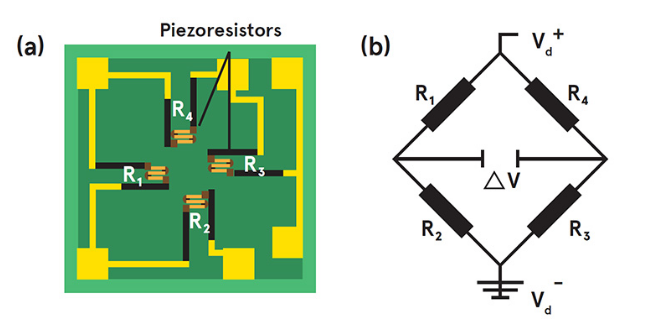
\includegraphics[width=0.7\textwidth]{img/barometro_wheatstone.png}
%     \caption{Puente de Wheatstone conformado por los resistores del sensor de presión. La imagen se extrajo de \cite{baro_3}.}
%     \label{fig:barometro_wheatstone}
% \end{figure}

% \begin{subequations}
%     \begin{align}
%         \Delta V &= (V_d^+ - V_d^-) \left[ \frac{R_2}{R_2 + R_1} - \frac{R_3}{R_3 + R_4} \right]\\
%         R_1 &= R_3 = R - \Delta R\\
%         R_2 &= R_4 = R + \Delta R\\
%         \Delta V &= (V_d^+ - V_d^-) \frac{\Delta R}{R}
%     \end{align}
%     \label{eq:barometro_wheatstone}
% \end{subequations}

% En la aplicación del vehículo aéreo, el barómetro se utiliza con el fin de medir la altura del vehículo, respecto de una altura inicial. La forma de medir la altitud a través de la presión es utilizando la ecuación de los gases nobles para el aire \cite{cavcar2000international}. En las ecuaciones \eqref{eq:gases_nobles} se obtiene una expresión para la presión, en función de la densidad del aire, la constantes de los gases y la masa molar del aire.

% \begin{subequations}
%     \begin{align}
%         P V &= n R T\\
%         n &= \frac{m}{M}\\
%         P V &= \frac{m}{M} R T\\
%         P &= \frac{m}{V} \frac{R T}{M}\\
%         P &= \rho \frac{R T}{M} \label{eq:presion_gas_nobles}
%     \end{align}
%     \label{eq:gases_nobles}
% \end{subequations}

% Luego, utilizando la condición hidrostática, la presión es la ejercida por la columna de aire \cite{cavcar2000international}. En la condición hidrostática de la ecuación \ref{eq:condicion_hidrostatica} se puede despejar la densidad del aire y reemplazarla en \eqref{eq:presion_gas_nobles}. Finalmente, se obtiene la ecuación diferencial de \eqref{eq:presion_diferencial}.

% \begin{equation}
%     dp = -\rho g dh
%     \label{eq:condicion_hidrostatica}
% \end{equation}

% \begin{equation}
%     \frac{dP}{P} = - \frac{g M}{R T} dh
%     \label{eq:presion_diferencial}
% \end{equation}

% Esta ecuación puede integrarse a ambos lados para hallar la relación entre la presión y la altura. Todos los términos de la ecuación \eqref{eq:presion_diferencial} son constantes, a excepción de la temperatura. Según el modelo \textit{International Standard Atmosphere} (ISA), se modela la relación entre la temperatura y la altitud, según la ecuación \eqref{eq:ISA_temperatura}. Esta relación es válida solamente hasta la estratósfera.

% \begin{subequations}
%     \begin{align}
%         T(h) &= T_0 + L \ h\\
%         T(h) &= 288.15 K - h \ 6.5 \ 10^{-3} m/K
%     \end{align}
%     \label{eq:ISA_temperatura}
% \end{subequations}

% Finalmente, se obtiene una expresión de la presión en función de la altura, ecuación \eqref{eq:ISA_presion}. 

% \begin{subequations}
%     \begin{align}
%         P(h) &= P_0 \left[ 1 + \frac{L h}{T_0} \right]^{-\frac{M g}{R L}}\\
%         P(h) &= 1013.25 \ hPa \left[ 1 - 0.0065 \frac{h}{288.15 K} \right]^{5.2561}
%     \end{align}
%     \label{eq:ISA_presion}
% \end{subequations}

% Se puede obtener un modelo más simplificado si se asume una temperatura constante, independiente de la altitud. Se reemplaza en \eqref{eq:presion_diferencial} y resolviendo la ecuación diferencial se obtiene la ecuación \eqref{eq:presion_temp_constante}.

% \begin{subequations}
%     \begin{align}
%         P(h) &= P_0 \ e^{-\frac{g M h}{R T}}\\
%         P(h) &= 1013.25 \ hPa \ e^{-\frac{h}{8840.2 m} }
%     \end{align}
%     \label{eq:presion_temp_constante}
% \end{subequations}

Al igual que con el sensor IMU, se hizo una búsqueda de las distintas alternativas. Los parámetros típicamente especificados son los siguientes:

\begin{itemize}
    \item \textit{Full-scale range}
    \item \textit{Absolute Accuracy}
    \item \textit{Relative Accuracy}
    \item \textit{Solder Drift}
    \item \textit{Offset vs temp}
    \item \textit{Offset vs time}
    \item \textit{Noise}
\end{itemize}

Como se puede ver, estos son similares a los de la IMU. Las diferencias se encuentran en los parámetros \textit{Absolute Accuracy}, \textit{Relative Accuracy} y \textit{Solder Drift}.\\

Se puede plantear un mismo modelo de medición según la ecuación \ref{eq:medicion_vs_real} pero para la presión.

\begin{equation}
    P_m = (1+S)P + P_b(t) + \eta
    \label{eq:medicion_presion}
\end{equation}

En el caso de la IMU, el parámetro \textit{scale factor error} se refiere al término $S$ y el \textit{offset} al término $P_b$. En el caso del barómetro, estos valores se encuentran especificados de otra manera. Si se quiere medir una presión $P$, el error de medición será $\Delta P = S \ P + P_b(t) + \eta$. El término $S \ P + P_b(t)$ corresponde al parámetro \textit{absolute accuracy} \cite{baro_4}. Este error es introducido debido a que la cavidad dentro del sensor no se encuentra a presión 0 perfecta, sino que a un pequeño valor \cite{baro_1}. Por otro lado, el término $S \ P$ se lo denomina \textit{relative accuracy}. Este hace referencia a mediciones diferenciales de presión. Algunos barómetros MEMS traen consigo una funcionalidad para realizar una compensación de offset. Esto dejaría como parámetro de interés para mediciones de presión a la \textit{relative accuracy}, la cual hace referencia al error introducido para mediciones de variaciones de presión.\\

El parámetro \textit{solder drfit} se refiere al offset que se introduce por el propio proceso de soldadura \cite{baro_4}. Este offset también puede ser compensado a través de la calibración del barómetro.\\

Se buscaron modelos de barómetros de distintos fabricantes, para comparar características, teniendo en cuenta la accesibilidad y el bajo costo. En la tabla \ref{tab:comparacion_baros} se muestra una comparación de los distintos barómetros considerados. Sumado a esto, se tuvo en consideración otro aspecto que fue mencionado anteriormente, la longevidad del componente.

\begin{table}[H]
    \centering
    \begin{tabular}{|c||c|c|c|c|c|c|}
        \hline
          & BMP390 & BMP581 & ICP-20100 & LPS22HH & ILPS22QSTR & DPS368\\
        \hline
        Full scale range [hPa] & 300 - 1250 & 300 - 1250 & 260 - 1260 & 260 - 1260 & \cellcolor{green!25}\makecell{260 - 1260 \\ 260 - 4060} & 300 - 1200\\ 
        absolute acc [hPa] & $\pm 0.5$ & $\pm 0.3$ & \cellcolor{green!25}$\pm 0.2$ & $\pm 0.5$ & $\pm 0.5$ & $\pm 1$\\
        realtive acc [hPa] & $\pm 0.03$ & $\pm 0.06$ & \cellcolor{green!25}$\pm 0.01$ & $\pm 0.025$ & $\pm 0.015$ & $\pm 0.06$\\
        \hline
        longevidad & N/A & N/A & N/A & N/A & \cellcolor{green!25}\makecell{10 años \\ enero 2023} & N/A \\
        \hline
        %AEC-Q100 & No & No & No & No & No & No\\
        %\hline       
    \end{tabular}
    \caption{Se muestra la comparación de las distintas alternativas que fueron tenidas en cuenta para la selección del sensor.}
    \label{tab:comparacion_baros}
\end{table}

Las dos alternativas que se evaluaron son los sensores ICP-20100 y el ILPS22QSTR. El primero de ellos presenta las \textit{absolute accuracy} y \textit{relative accuracy} más bajas de entre todas las opciones evaluadas. El sensor ILPS22QSTR presenta características similares y además tiene la particularidad de que el fabricante garantiza su fabricación por 10 años, hasta enero de 2033 \cite{baro_5}. Finalmente el sensor seleccionado fue este último.

En este caso también se tomó como guía el circuito de la hoja de datos del componente. La interfaz de comunicación seleccionada es I2C. Se prefiere utilizar I2C en lugar de SPI ya que puede aprovecharse el uso del mismo bus al que se conecta el barómetro, para conectar otros sensores y dispositivos. De esta manera, se ahorra la cantidad de pistas y conexiones en el diseño del PCB. Si bien I2C tiene un funcionamiento más lento que SPI, las mediciones del barómetro no son tan críticas como las de la IMU. Este sensor, a diferencia de la IMU, no cuenta con una línea de interrupción, por lo que los datos deben obtenerse por \textit{polling} de forma peródica. El circuito completo puede encontrarse en el \nameref{appendix:circuito_esquematico}.

\subsubsection{Magnetómetro}
%\subsection{Magnetómetro}

El magnetómetro es otro de los sensores complementarios al INS. Este se utiliza para obtener estimaciones del ángulo de \textit{yaw} del vehículo, a partir de mediciones del campo magnético terrestre. Estas mediciones son relativas a una terna solidaria al sensor. Esto se muestra en la figura  . Luego el ángulo de \textit{yaw} puede obtenerse a partir del ángulo entre las componentes en $H_y$ y $H_x$.

\textbf{{\color{red} AGREGAR UNA IMAGEN DEL CAMPO MAGNÉTICO MEDIDO POR EL MAGNETÓMETRO CON SUS COMPONENTES}}

Para medir las componentes del campo magnético, el sensor utiliza una serie de materiales resistivos que son sensibles al campo magnético aplicado sobre estos. Se colocan 4 resistores en configuración puente de Wheatstone y se estiman las componentes del campo magnético a partir del desbalance de este.

Para la selección del componente se hicieron comparaciones de las características de varias alternativas. Los parámetros típicamente especificados para el magnetómetro son los siguientes:

\begin{itemize}
    \item \textit{Full-scale range}
    \item \textit{Scale Factor Error}
    \item \textit{Scale Factor Error vs Temp}
    \item \textit{Offset}
    \item \textit{Offset vs temp}
    \item \textit{Noise}
\end{itemize}

Se buscaron modelos de magnetómetros disponibles. Al igual que con el resto de componentes, se redujo la búsqueda a aquellos que sean de bajo costo. En la tabla  se muestra una comparativa de los modelos considerados para la selección final.

\begin{table}[H]
    \centering
    \begin{tabular}{|c||c|c|c|c|}
        \hline
          & HMC5883L & BMM150 & RM3100 & MMC5983MA\\
        \hline
        %Full scale range [uT] & \makecell{$\pm$88;130;190;250;\\400;470;560;810} & \makecell{x,y: $\pm$1200;\\z: $\pm$2000} & $\pm$800 & $\pm$800\\
        Scale Factor Error & $\pm$0,1 \% @ $\pm$200 uT & 1\% & $\pm$0,5\% @ $\pm$200 uT & \cellcolor{green!25}0,1\% @ $\pm$400uT\\
        \hline
        \makecell{Scale Factor Error\\Over Temp} & \makecell{0.3\%/C \\@ -40°C - 125 °C} & N/A & N/A & \cellcolor{green!25}\makecell{0.07 \%/°C \\@ -40°C - 105°C}\\
        \hline
        Offset @25°C & N/A & \cellcolor{green!25}$\pm$ 40 uT & N/A & $\pm$50 uT\\
        \hline
        Offset Over Temp & N/A & N/A & N/A & \cellcolor{green!25}\makecell{$\pm$2nT/°C \\@ -40°C - 105°C}\\
        \hline
        Noise & \makecell{200 nT \\@ FSR = $\pm$88 uT} & \makecell{300 nT @ 25°C,\\ ODR = 20 Hz} & \cellcolor{green!25}30 nT & \makecell{40nT @ ODR = 50 Hz\\60 nT @ ODR = 100 Hz\\80 nT @ ODR = 200 Hz\\120 nT @ ODR = 400 Hz}\\
        \hline
        AEC-Q100 & No & No & No & \cellcolor{green!25}Sí\\
        \hline
    \end{tabular}
    \caption{Se muestra la comparación de las distintas alternativas que fueron tenidas en cuenta para la selección del magnetómetro. En verde se destaca el modelo con las mejores prestaciones para cada especificación.}
    \label{tab:comparacion_mags}
\end{table}

El modelo RM3100 es el que posee el nivel más bajo de ruido. Este componente se utiliza en computadoras de vuelo comerciales, pero además fue utilizado con éxito en el proyceto Artemis de la NASA. A pesar de las bondades que ofrece, el costo de este componente en el momento de la selección era entre 5 a 10 veces superior con respecto a los otros. Finalmente el sensor elegido fue el modelo MMC5983MA. Este es el único de todas las alternativas consideradas que contiene información de todos los parámetros. Además de tener unas muy buenas características, el mismo es de grado automotriz, lo que le da todavía más robustez.

El efecto del campo magnético producido por los motores del UAV afectan las mediciones del sensor, volviéndolo prácticamente inutilizable para la navegación del vehículo. Para evitar este problema, el magnetómetro se montará en una posición elevada respecto de la computadora de vuelo. Esto quiere decir que este sensor no se montará sobre la placa, sino que se conectará como un sensor externo, utilizando alguno de los concetores de la placa.

\subsubsection{Interfaz de Comunicación CAN}
%\subsection{Interfaz de Comunicación CAN}

% Como fue mencionado, la computadora de vuelo cuenta con la capacidad de conexión a un bus CAN. La especificación original del protocolo \cite{specification1991bosch} incluye dentro de sus definiciones, la capa física. Cada nodo de un bus CAN se conecta a este a través de 2 cables, los cuales llevan la señal diferencial. Esto se muestra en la figura \ref{fig:conxeion_al_bus_CAN}. Todo el bus CAN se compone de 2 cables que llevan los mensajes a todos los nodos de la red. Esto es así debido a que el bus CAN originalmente fue diseñado para utilizarse en automóviles y reemplazar la enorme cantidad de conexiones entre módulos. El hecho de que se trate de una señal diferencial hace que la comunicación sea robusta, reduciendo las emisiones electromagnéticas generadas por este. A su vez, es común que el bus sea cableado como un par trenzado, lo que atenúa señales de modo común, producto de cualquier acoplamiento. 

% \begin{figure}[H]
%     \centering
%     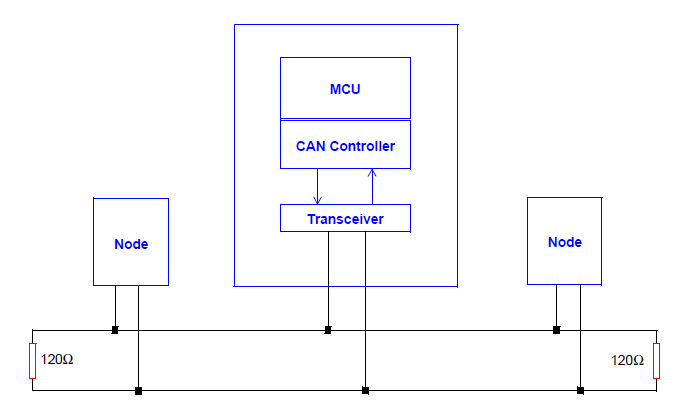
\includegraphics[width=0.5\textwidth]{img/conxeion_al_bus_CAN.png}
%     \caption{La conexión de un nodo al bus es a través de 2 cables que llevan dos señales, CAN-H y CAN-L. La imagen se extrajo de \cite{AN228}.}
%     \label{fig:conxeion_al_bus_CAN}    
% \end{figure}

% Existen muchas versiones del protocolo CAN, en este trabajo se utiliza la versión CAN High Speed. Esta define una velocidad máxima de transferencia de 1 Mbps, para un bus de hasta 40 m de longitud y 30 nodos conectados al mismo bus. Se recomienda que la conexión entre cada nodo y el bus no sea de más de 30 cm. El hecho de poder tener hasta 30 nodos expande las posibilidades de uso del bus, más allá de ser el medio principal de comunicación utilizado para el sistema redundante. Por ejemplo, distintos sensores o incluso actuadores como los motores del vehículo podrían conectarse al bus. {\color{red} Acá tendría que agregar alguna referencia a este uso del bus CAN}.\\

% La impedancia característica del bus debe ser de $120 \ \Omega$. Es común agregar resistores de terminación en ambos extremos, para evitar reflexiones. En algunos casos pueden llegar a encontrarse aplicaciones donde los resistores de terminación se incluyen dentro de alguno de los nodos del bus. Esto no es recomendable, ya que si este se desconecta de forma accidental del bus, todas las comunicaciones entre los demás nodos se verán perjudicadas. Este es el motivo por el cual la computadora de vuelo no incluye este resistor en el circuito.\\

% En la figura \ref{fig:conxeion_al_bus_CAN} se muestran 2 elementos que forman parte del nodo, el \textit{trasnciever} y el \textit{controller}. El primero de ellos forma parte de la capa física y es un circuito que convierte las señales diferenciales del bus en señales de modo común, que luego son transferidas al elemento \textit{controller}. Este componente sirve como interfaz física con el bus.\\

Como ya fue mencionado, la computadora de vuelo requiere que la comunicación entre sus réplicas sea través de un bus. Para ello, la placa debe contar con un circuito con una interfaz de comunicación con el mismo. A partir de lo presentado hasta aquí, el único requerimiento es el método de acceso al medio, el cual debe ser controlado por el tiempo. Teniendo en cuenta que se trata de un trabajo realizado con componentes COTS, el hardware a utilizar debe ser de fácil acceso y con costos razonables. Para el desarrollo de este trabajo, se seleccionó el bus \textit{Controller Area Network} (CAN)\cite{specification1991bosch}. Si bien su método de acceso al medio no es TDMA, existe una extensión del protocolo que justamente busca incorporar esta funcionalidad en otra capa superior.

%En las secciones siguientes se explica un inconveniente, en cuanto a la selección del microcontrolador. 

%El microcontrolador que se utiliza cuenta con un periférico que permite utilizar una interfaz con este bus. A continuación se presentan brevemente algunas características.

%Si bien el método de acceso al medio no es TDMA, existe una extensión del protocolo que justamente busca incorporar esta funcionalidad en otra capa superior.

%\subsubsection{Descripción del Protocolo CAN}

El protocolo CAN fue desarrollado para ser usado en la industria automotriz, como bus de comunicación que conecta distintos módulos dentro de un automóvil. El objetivo de su desarrollo fue similiar al motivo por el cual se desarrolló el bus ARINC 629 en aviones, reemplazar la gran cantidad de cables dentro del vehículo por un bus simple. El protocolo se corresponde con el modelo OSI y la especificación original define las capas física y de enlace.

A diferencia de otros protocolos típicos en sistemas embebidos como I2C o SPI, el protocolo CAN no tiene el formato maestro-esclavo. La comunicación se da entre miembros del bus denominados nodos, los cuales se encuentran conectados a los mismos 2 cables. Esto se muestra en la figura \ref{fig:red_CAN_2}. 

\begin{figure}[H]
    \centering
    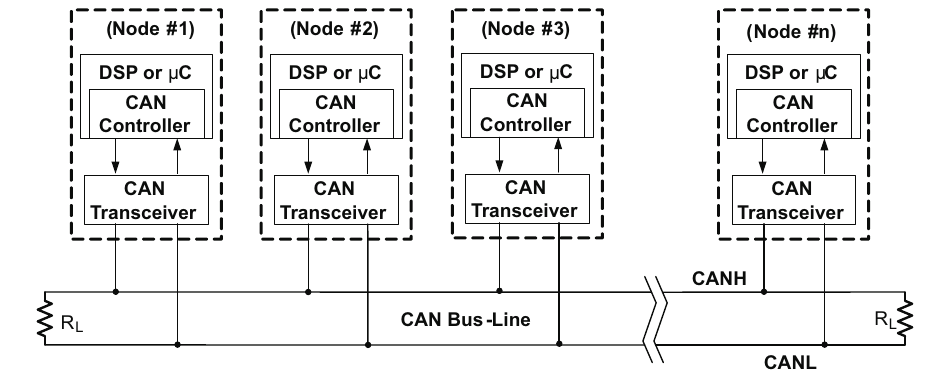
\includegraphics[width=\textwidth]{img/red_CAN.png}
    \caption{Todos los nodos se encuentran conectados al mismo bus de comunicaciones. El bus CAN se compone de dos cables, CAN-H y CAN-L, terminados en sus extremos por resistencias de adaptación. La imagen se extrajo de \cite{texasSLOA101B}.}
    \label{fig:red_CAN_2}
\end{figure}

La impedancia característica del bus debe ser de $120 \ \Omega$. Es común agregar resistores de terminación en ambos extremos, para evitar reflexiones. En algunos casos pueden llegar a encontrarse aplicaciones donde los resistores de terminación se incluyen dentro de alguno de los nodos del bus. Esto no es recomendable, ya que si el mismo se desconecta de forma accidental del bus, todas las comunicaciones entre los demás nodos se verán perjudicadas debido a la pérdida del resistor de adaptación.

La información enviada por los nodos a través de estos 2 cables es en formato de señal diferencial, lo que vuelve robusta a la comunicación, reduciendo las emisiones electromagnéticas generadas por este. A su vez, es común que el bus sea cableado como un par trenzado, lo que atenúa señales de modo común, producto de cualquier acoplamiento.

\textbf{{\color{red} AGREGAR UNA IMAGEN DE OCSILOCSOPIO DONDE SE VEAN LAS SEÑALES DIFERENCIALES DE CAN.}}

El protocolo CAN define dos estados para el bus, \textit{recessive} y \textit{dominant}. Cuando no hay actividad en el bus, tanto la línea de CAN-H como la de CAN-L se encuentran a la misma tensión constante. Esto corresponde al estado \textit{recessive} y equivale a un 1 lógico. Cuando se quiere enviar un 0 lógico, el transciever del nodo transmisor fija la tensión de las líneas CAN-H y CAN-L de tal forma de generar una tensión diferencial $V_{CAN-H} - V_{CAN-L} \geq 1,5 V$. Esto se muestra en la figura \ref{fig:CAN_recessive_dominant}.

\begin{figure}[H]
    \centering
    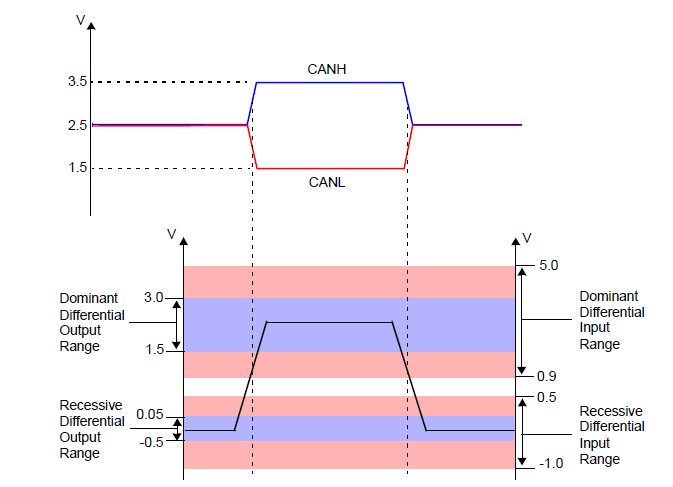
\includegraphics[width=0.7\textwidth]{img/CAN_recessive_dominant.png}
    \caption{Se muestran los estados recessive y dominant del bus CAN y sus equivalentes lógicos.}
    \label{fig:CAN_recessive_dominant}    
\end{figure}

Los nodos solamente actúan sobre el bus cuando quieren fijar un estado \textit{dominant}. Cuando se quiere fijar un estado \textit{recessive}, no se actúa sobre el bus ya que este es su estado por defecto. Esto permite que varios nodos puedan actuar al mismo tiempo. En caso de que esto suceda, el estado \textit{dominant} (de allí su nombre) predominará sobre el estado \textit{recessive}.

Existen muchas versiones del protocolo CAN, en este trabajo se utiliza la versión CAN High Speed. Esta define una velocidad máxima de transferencia de 1 Mbps, para un bus de hasta 40 m de longitud y 30 nodos conectados. Se recomienda que la conexión entre cada nodo y el bus no sea de más de 30 cm. El hecho de poder contar con hasta 30 nodos expande las posibilidades de uso, más allá de ser el medio principal de comunicación utilizado para el sistema redundante. Por ejemplo, distintos sensores o incluso actuadores como los motores del vehículo podrían conectarse al bus. {\color{red} Acá tendría que agregar alguna referencia a este uso del bus CAN}.

%Cada nodo de un bus CAN se conecta a este a través de 2 cables, los cuales llevan la señal diferencial. Esto se muestra en la figura \ref{fig:conxeion_al_bus_CAN}. Todo el bus CAN se compone de 2 cables que llevan los mensajes a todos los nodos de la red. 

% \begin{figure}[H]
%     \centering
%     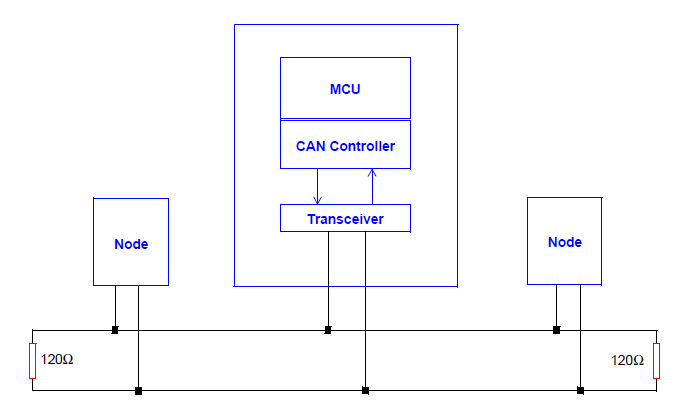
\includegraphics[width=0.5\textwidth]{img/conxeion_al_bus_CAN.png}
%     \caption{La conexión de un nodo al bus es a través de 2 cables que llevan dos señales, CAN-H y CAN-L. La imagen se extrajo de \cite{AN228}.}
%     \label{fig:conxeion_al_bus_CAN}    
% \end{figure}

%Existen muchas versiones del protocolo CAN, en este trabajo se utiliza la versión CAN High Speed. Esta define una velocidad máxima de transferencia de 1 Mbps, para un bus de hasta 40 m de longitud y 30 nodos conectados al mismo bus. Se recomienda que la conexión entre cada nodo y el bus no sea de más de 30 cm. El hecho de poder tener hasta 30 nodos expande las posibilidades de uso del bus, más allá de ser el medio principal de comunicación utilizado para el sistema redundante. Por ejemplo, distintos sensores o incluso actuadores como los motores del vehículo podrían conectarse al bus. {\color{red} Acá tendría que agregar alguna referencia a este uso del bus CAN}.\\

En la figura \ref{fig:red_CAN_2} se muestra que cada nodo se compone de 2 elementos, el \textit{trasnciever} y el \textit{controller}. El primero de ellos forma parte de la capa física y es un circuito que convierte las señales diferenciales del bus en señales de modo común. Luego las señales de modo común son transferidas al elemento \textit{controller}. Este típicamente se encuentra implementado en hardware dentro de una unidad de procesamiento como un microcontrolador, como es el caso de este trabajo.

%En la figura \ref{fig:red_CAN_2} se muestran 2 elementos que forman parte del nodo, el \textit{trasnciever} y el \textit{controller}. El primero de ellos forma parte de la capa física y es un circuito que convierte las señales diferenciales del bus en señales de modo común, que luego son transferidas al elemento \textit{controller}. Este componente sirve como interfaz física con el bus.\\

% Formato de la tama CAN

Una trama del protocolo CAN se comopone de varios campos. Además, se definen 2 tipos de tramas, estándar, figura \ref{fig:CAN_frame_standard} y extended, figura \ref{fig:CAN_frame_extended}.

\begin{figure}[H]
    \centering
    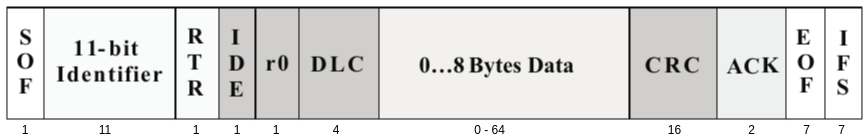
\includegraphics[width=0.8\textwidth]{img/CAN_frame_standard.png}
    \caption{Se muestran los campos de una trama CAN estándar. Debajo de cada campo se indica la cantidad de bits. La imagen se extrajo de \cite{texasSLOA101B}.}
    \label{fig:CAN_frame_standard}
\end{figure}

\begin{itemize}
    \item SOF: Inicio de una nueva trama en el bus.
    \item Identifier: Indica el contenido del campo de datos.
    \item RTR: Dominante para \textit{data frames}, recessive para \textit{remote frames}. Estas últimas se utilizan para solicitar a otro nodo que envíe determinado mensaje. Su formato es el mismo, solo que no pueden contener bytes en su campo de datos.
    \item IDE: Si es dominante, se trata de una trama estándar. Si no, es una trama extended.
    \item r0: Reservado.
    \item DLC: Cantidad de bytes de datos enviados.
    \item Data: Datos útiles, entre 0 y 8 bytes.
    \item CRC: Chequeo de la integridad del mensaje de la trama.
    \item ACK: Se compone de 2 bits denominados ACK SLOT Y ACK DELIMITER. El emisor deja estos campos en recessive y cuando algún nodo recibe el mensaje, fuerza un nivel dominant en el bus, indicando que se recibió el mensaje correctamente.
    \item EOF: Fin de trama.
    \item IFS: Espacio antes de enviar la próxima trama, de 7 bits. 
\end{itemize}

\begin{figure}[H]
    \centering
    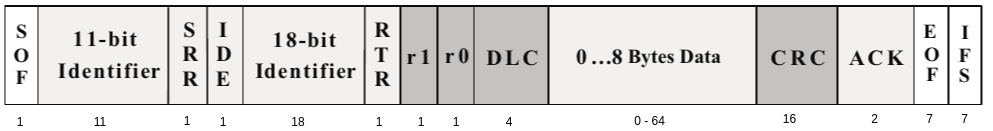
\includegraphics[width=0.8\textwidth]{img/CAN_frame_extended.png}
    \caption{Se muestran los campos de una trama CAN extendida. Debajo de cada campo se indica la cantidad de bits. La imagen se extrajo de \cite{texasSLOA101B}.}
    \label{fig:CAN_frame_extended}
\end{figure}

La trama extended mantiene los mismos campos pero incorpora otros 2 más:

\begin{itemize}
    \item SRR: Debe ser recessive para extended frames.
    \item r1: Reservado.
\end{itemize}

% Acceso al medio


%CAN es un protocolo donde no hay un nodo master, sino que todos pueden utilizar el medio para transmitir mensajes, 
Debido a que no existe un nodo que sea maestro, todos los miembros del bus pueden iniciar la transmisión de un mensaje. El método de acceso al medio se denomina \textit{Carrer Sense Multiple Access with Collision Detection and Arbitration on Message Priority} (CSMA/CD+AMP). Antes de transmitir un mensaje, el nodo sensa el bus y en caso de que esté libre, intenta utilizarlo para transmitir un mensaje.

%En caso de que más de un nodo quiera enviar un mensaje a la vez, esto llevará a una colisión. El protocolo tiene un método para solucionar las colisiones sin tener pérdida de mensajes.

En el eventual caso en que más de un nodo detecte el medio sin uso, estos intentarán transmitir a través del bus al mismo tiempo. Esta situación se encuentra contemplada por el protocolo a través de un mecanismo que resuelve la colisión mientras que asegura la transmisión del mensaje con la prioridad más alta. El mensaje con la prioridad más alta será aquel que tenga en su campo Identifier el valor más bajo. De aquí se desprende la necesidad de que en un mismo bus no haya mensajes distintos con el mismo campo ID.

En la figura \ref{fig:CAN_arbitration} se muestra un ejemplo donde se resuelve una colisión. Tanto el nodo 1 como el nodo 2 quieren utilizar el bus CAN. Ambos comienzan a inyectar su ID correspondiente. En algún momento, ocurre una discrepancia entre el ID inyectado por ambos nodos. Aquel con el campo dominant, es decir 0, gana y completa su transmisión, en este caso el nodo 2. El nodo 1 que quiso enviar un 1 por su lado, detecta un 0. Esto genera que detenga su transmisión, dejando que los demás nodos utilicen el medio.

\begin{figure}[H]
    \centering
    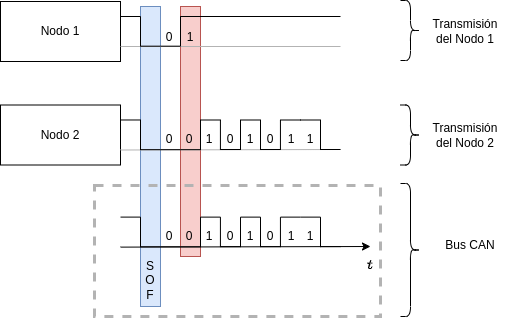
\includegraphics[width=0.6\textwidth]{img/CAN_arbitration.png}
    \caption{Mecanismo para la detección de colisiones. El nodo 2 gana por prioridad y completa su transmisión, mientras que el nodo 1 deja de usar el bus, aguardando a que el nodo 2 finalice.}
    \label{fig:CAN_arbitration}
\end{figure}

%En las figuras \ref{fig:CAN_frame_standard} y \ref{fig:CAN_frame_extended} se puede ver que las tramas tienen un campo CRC, el cual es utilizado para que el receptor pueda verificar la integridad del mensaje. Además, se muestra otro campo, el ACK. Cada vez que un nodo recibe un mensaje correctamente, este sobreescribe el bit de ACK con un dominant, es decir un 0.\\

El protocolo CAN de por sí, no cuenta con un acceso al medio controlado por el tiempo, sino que es dominado por eventos (\textit{event-triggered}), ya que varios nodos pueden iniciar la transmisión de un mensaje en cualquier momento. En el estándar ISO 11898-4\cite{ISO11898_4} se define una extensión del protocolo CAN denominada \textit{Time-Triggered CAN} (TTCAN). Esta justamente fue desarrollada con el objetivo de utilizar el protocolo en aplicaciones de alta confiabilidad. Para ello, TTCAN incorpora un mecanismo de comunicación entre nodos a través de un scheduling estático, el cual es respetado por todos. A cada mensaje del scheduling se le asigna una ventana de tiempo y el mismo se repite de forma periódica.\\

%Al utilizar un scheduling estático, se evitan las colisiones y las retransmisiones. Teniendo en cuenta que se trata de sistemas de alta confiabilidad, una colisión en el bus puede traer consigo el retraso en la transmisión de mensajes críticos para el desempeño del sistema y la seguridad. El scheduling de los mensajes y los tiempos en que estos se envían pasan a formar parte del diseño del sistema.

%Como se mencionó al principio de la sección \ref{sec:requerimentos_sistema_tolerancia_fallas}, la arquitectura para la tolerancia a fallas no está definida. 
%La elección del protocolo CAN le da versatilidad al uso del bus, ya que puede utilizarse con un acceso al medio tanto controlado por el tiempo como por eventos.

%En la figura \ref{fig:microcontrolador_transciever} se muestra la comunicación entre transciever, controller y el bus. Cuando se quiere transferir un mensaje a través del bus CAN, el periférico envía un mensaje a través del terminal CAN TX. El transciever lo recibe y lo convierte en una señal diferencial para inyectarlo en el bus. Cuando el nodo recibe un mensaje del bus CAN, el transciever es el que interactúa con el bus y genera una señal de modo común, la cual es enviada a través del terminal CAN RX al microcontrolador.

% \begin{figure}[H]
%     \centering
%     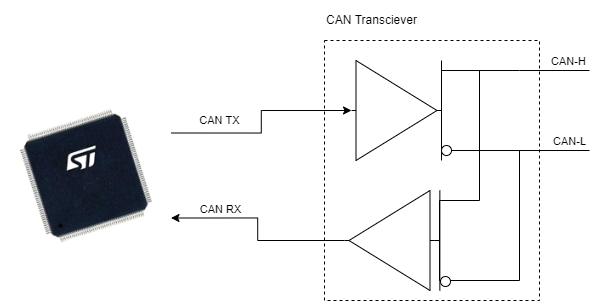
\includegraphics[width=0.5\textwidth]{img/microcontrolador_transciever.png}    
%     \caption{El periférico embebido en el microcontrolador, a través del transciever, puede interactuar con el bus CAN.}
%     \label{fig:microcontrolador_transciever}
% \end{figure}



%La interfaz CAN se compone del transciever, su comunicación con el microcontrolador y el conector.

El micronotrolador seleccionado para la computadora de vuelo, cuenta con 2 \textit{controller} embebido, el periférico bxCAN \cite{STM32F746ZG}. Cada uno de ellos cuenta con 2 líneas de comunicación con el transciever, CAN TX y CAN RX, las cuales se utilizan para enviar y recibir las señales de modo común al \textit{trasnciever}. En cuanto a este útlimo, se trata de un componente que es ampliamente utilizado en la electrónica automotriz, por lo que hay mucha disponibilidad. Existen transcievers que utilizan distintos niveles de tensión en sus salidas. La gran mayoría de los componentes de la computadora de vuelo utilizan tensiones de 3,3 V para su funcionamiento, por lo que se buscó algún componente que pueda trabajar con este nivel de tensión. El componente seleccionado es el SN65HVD230 de Texas Instruments \cite{SN65VHD230}, el cual es compatible con la especificación de capa física de CAN, ISO 11898-2. En la figura \ref{fig:microcontrolador_transciever} se muestra la comunicación del microcontrolador con el bus CAN a través del \textit{transciever}. Este cuenta con una protección por exceso de tempertura, donde el componente pone sus salidas CAN-H y CAN-L en alta impdeancia, de manera de no perturbar al resto de los nodos. Además, cuenta con una funcionalidad que permite detectar si el transciever fue desconectado del bus, fijando un estado alto constante en su salida RX hacia el \textit{controller}, informándole de la situación.

\begin{figure}[H]
    \centering
    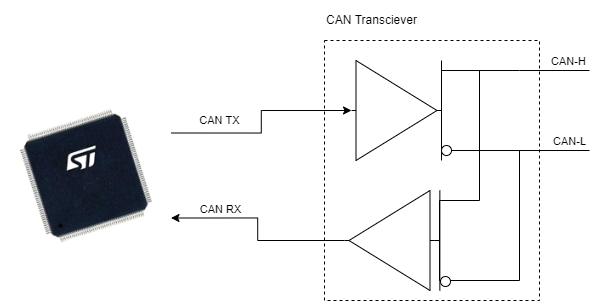
\includegraphics[width=0.5\textwidth]{img/microcontrolador_transciever.png}    
    \caption{Se muestran las conexiones entre el \textit{controller} embebido en el microcontroldaor y el \textit{transciever}, a través de las líneas CAN TX y CAN RX. {\color{red} CAMBIAR ESTA IMAGEN POR UNA MÁS CLARA Y PROLIJA}}
    \label{fig:microcontrolador_transciever}
\end{figure}

Como se muestra en la figura \ref{fig:microcontrolador_transciever}, el \textit{transciever} cuenta con un terminal \textit{Rs} que permite controlar el tiempo de crecimiento y de decrecimiento de las líneas CAN-H y CAN-L. Al realentizar el tiempo de crecimiento en las líneas CAN-H y CAN-L, se atenúa el contenido armónico de las más altas frecuencias, disminuyendo emisiones. Por ejemplo, si se coloca un resistor de $10 \ k\Omega$ en el terminal 8 denominado \textit{Rs}, la hoja de datos indica un slew-rate de $15 \ V / \mu s$.

La especificación de la capa física de CAN no indica un conector a utilizar. Se buscó seleccionar alguno que no ocupe demasiado espacio al ser montado en el PCB. En \cite{CiAconnector} se mencionan algunas recomendaciones de conectores. Este es un documento publicado por la organización internacional sin fines de lucro, \textit{CAN in Automation}, que se dedica a publicar recomendaciones y especificaciones relacionadas al uso del bus CAN. Dentro de las opciones que da este documento, se buscó alguno que tenga dimensiones razonables a lo requerido para la placa. De entre todas las opciones se seleccionó el conector que corresponde a la especificación de un protocolo CAN desarrollado para ser usado en drones, DroneCAN \cite{DroneCAN}, el conector JST GH 4. Por cuestiones de disponibilidad, se seleccionó otro componente similar a este y que es del mismo fabricante de otros de los conectores utilizados para la computadora de vuelo, correspondiente a la serie DF-13 del fabricante Hirose. Este puede ver en la figura \ref{fig:conector_CAN}. Se utilizaron dos de estos conectores, uno por cada \textit{transciever}. Al ser de pequeñas dimensiones, la inclusión de ambos conectores no ocupa demasiado espacio en la placa.

%\textbf{{\color{red} AGREGAR UNA IMAGEN DEL CONECTOR DF13 DE CAN.}}

\begin{figure}[H]
    \centering
    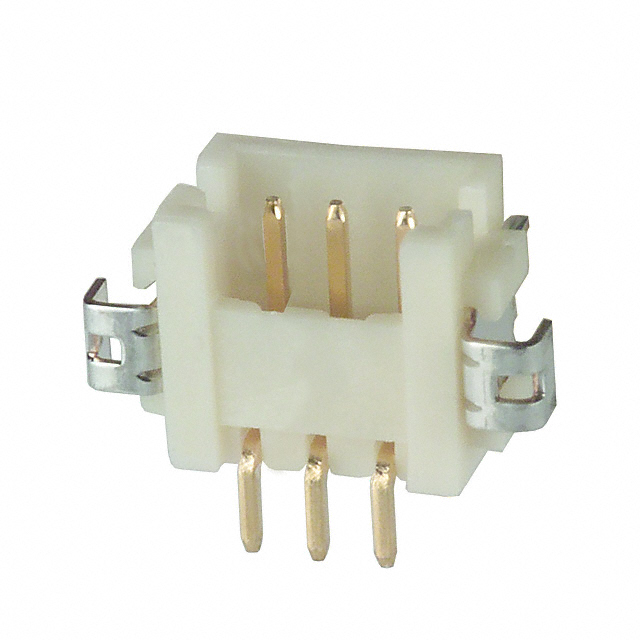
\includegraphics[width=0.2\textwidth]{img/conector_CAN.jpg}    
    \caption{Se muestra el conector utilizado para las interfaces CAN. El mismo cuenta con 3 terminales, de los cuales 2 de se utilizaron para la señal CAN diferencia. El terminal restante corresponde al GND de la placa.}
    \label{fig:conector_CAN}
\end{figure}

En cuanto al circuito implementado, se tomaron como punto de partida las recomendaciones de la hoja de datos del trasnciever SN65HVD230. Este recomienda el agregado de capacitores de desacople en las líneas de alimentación. %Además, se agregaron resistores en serie con las líneas de CAN RX y CAN TX, es decir, en las pistas que llevan las señales que van desde el controller al transciever y viceversa. Esto se hizo como medida preventiva para amortiguar las señales, en caso de que estas presenten sobrepicos en las conmutaciones. A priori se fijan en $0 \ \Omega$ y se modificarán de ser necesario.
El circuito completo de la interfaz CAN puede encontrarse en el \nameref{appendix:circuito_esquematico}.

%\textbf{{\color{red} COMPLETAR EL ANÁLISIS DEL MODELO DE PARÁMETROS CONCENTRADOS, PARA LAS PISTAS CAN-TX Y CAN-RX, PARA CALCULAR EL EVENTUAL RESISTOR EN SERIE.}}

%\subsection{Selección del Bus de Comunicaciones de la Computadora de Vuelo}



\subsubsection{Circuito de Alimentación}
%\subsection{Circuito de Alimentación}

Para alimentar el microcontrolador y los demás componentes, se incluye una fuente de alimentación de $3.3 \ V$. En las primeras dos versiones de la computadora de vuelo, desarrolladas por el LAR en trabajos anteriores, se integró una fuente conmutada de salida $5 \ V$ junto con un regulador lineal de $3.3 \ V$. A partir de la tercera versión, esta fuente conmutada se eliminó dejando solamente el regulador lineal de $3.3 \ V$ \cite{garberoglio2019diseno}. El motivo principal fue reducir las dimensiones de la placa y simplificar el diseño. Siguiendo esta misma línea, la fuente conmutada tampoco se incluyó en este trabajo. Se incorporó un conector, de manera de poder alimentar la placa utilizando una fuente externa de $5 \ V$.\\

El circuito implementado se comprende del regulador lineal, junto con capacitores de entrada y de salida. Para la selección del componente se buscó un regulador que sea de grado automotriz, por cuestiones de confiabilidad ya mencionadas, pero además se buscó un componente con un encapsulado SOT-223-3, figura \ref{fig:sot_223_3}. En el mercado local puede encontrarse una gran variedad de reguladores con este encapsulado, pensando en la necesidad de modificar el circuito, utilizando otro regulador o en caso de que haya que reemplazarlo.\\

\begin{figure}[H]
    \centering
    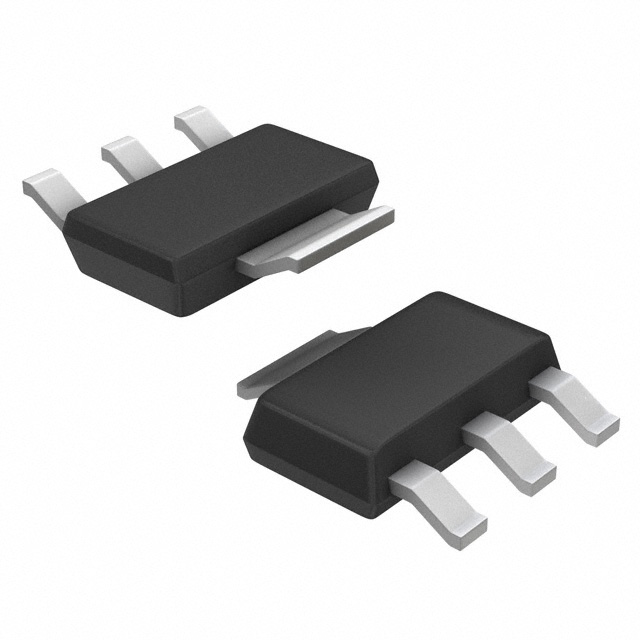
\includegraphics[width=0.3\textwidth]{img/sot_223_3.png}
    \caption{Encapsulado SOT-223-3 seleccionado para el regulador lineal. El terminal de mayor tamaño se encuentra conectado al terminal de tensión de salida, $3.3 \ V$.}
    \label{fig:sot_223_3}
\end{figure}

El chip seleccionado es el ZLDO1117QG33TA de DIODES Incorporated \cite{ZLDO1117QG33TA}, un regulador low-dropout de grado automotriz. Se siguió el circuito recomendado por la hoja de datos del fabricante, donde se coloca un capacitor a la entrada del regulador y otro en su salida.\\

La principal función del capacitor de entrada es la de proveer corriente al regulador, en caso de que ocurra un escalón en la corriente consumida por la carga del regulador \cite{TOSHIBALDO}. Este capacitor ayuda a mantener la tensión de entrada del regulador, en caso de que la fuente conectada a la entrada del regulador presente un drop-out. Se seleccionó un capacitor cerámico multicapa de valor $4.7 \ \mu F$. Este tipo de capacitores tienen una ESR muy baja, lo que permite que se descarguen rápido, en caso de que tengan que entregar carga para mantener la tensión de entrada en el regulador.\\

En cuanto al capacitor de salida, este cumple una doble función. Por un lado, aportar a la regulación de línea. Este parámetro es importante teniendo en cuenta que el regulador se utiliza para alimentar un circuito digital, donde aparecen muchas variaciones de corriente. En el caso en el que ocurra un cambio brusco de la corriente de salida del regulador, el capacitor de salida se descargará en parte, para intentar mantener la tensión de salida en un valor constante. Por otro lado, este capacitor también es utilizado para la compensación del regulador \cite{TOSHIBALDO}. En la figura \ref{fig:LDO_diagrama_bloques} se muestra un diagrama en bloques simplificado para un regulador lineal, donde puede verse que se trata de un sistema a lazo cerrado.

\begin{figure}[H]
    \centering
    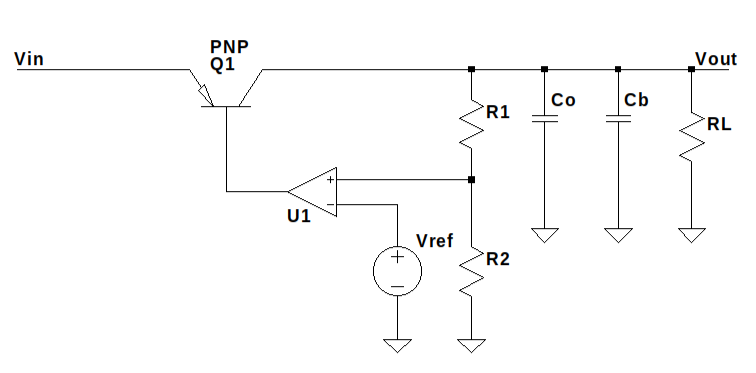
\includegraphics[width=0.7\textwidth]{img/LDO_diagrama_bloques.png}
    \caption{Diagrama en bloques de un regulador lineal. Este se compone de un transistor de paso, un amplificador de error, una tensión de referencia y un bloque realimentador, formado por $R_1$ y $R_2$. En el diagrama además se muestra $R_L$ que simboliza una carga resistiva y dos capacitores $C_o$ y $C_b$. Estos elementos forman un circuito a lazo cerrado que estabiliza la tensión de salida $V_{out}$.}
    \label{fig:LDO_diagrama_bloques}    
\end{figure}

Para analizar la ganancia de lazo, se plantea el esquema de realimentación en la figura \ref{fig:LDO_esquema_realimentacion}. Para el transistor de paso, se utiliza su modelo de pequeña señal. 

\begin{figure}[H]
    \centering
    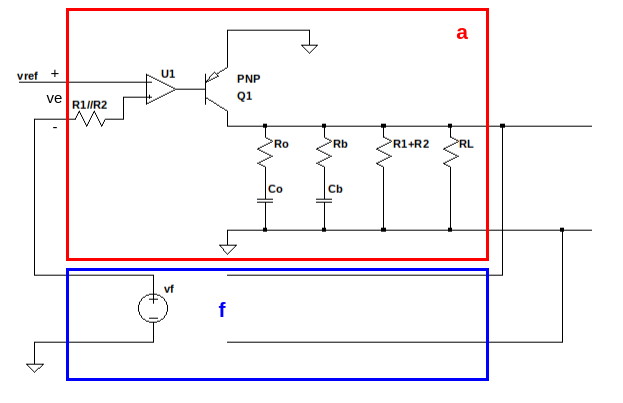
\includegraphics[width=0.8\textwidth]{img/LDO_esquema_realimentacion.png}
    \caption{Circuito equivalente para analizar la realimentación del regulador lineal. La tensión $v_{in}$ se pasiva ya que se analiza el circuito en el punto de operación.}
    \label{fig:LDO_esquema_realimentacion}    
\end{figure}

Se trata de un esquema que muestrea tensión y suma tensión. El bloque \textit{f} es tal que cumple con la relación de la ecuación \eqref{eq:LDO_bloque_f}. En cuanto al bloque \textit{a}, la transferencia corresponde a la ecuación \eqref{eq:LDO_bloque_a}, donde se ha asumido que $R_b \rightarrow 0$ por ser la ESR de un capacitor cerámico multicapa, $R_L \ll r_o$ y $R_L \ll (R_1+R_2)$. Además, se asume que $R_o \ll R_L$.

\begin{subequations}
    \begin{align}
        v_f &= f \ v_o\\
        f &= \frac{R_2}{R_1 + R_2} \label{eq:LDO_bloque_f}
    \end{align}
\end{subequations}

\begin{subequations}
    \begin{align}
        v_o &= a \ v_{ref}\\
        a &= A_v(s) g_m  R_L \frac{1 + s C_o R_o}{\left( 1 + s C_o  R_L \right)  \left( 1 + s C_b R_o \right)} \label{eq:LDO_bloque_a}
    \end{align}
\end{subequations}

La transferencia $A_v(s)$ corresponde al amplificador de error y se modela como de un polo simple. Juntando los bloques $a$ y $f$ puede obtenerse la ganancia de lazo para analizar la estabilidad, ecuación \eqref{eq:LDO_ganancia_lazo}. Esta se compone de 3 polos y 1 cero. Este último junto con uno de los polos dependen directamente del valor $R_o$, es decir, la ESR del capacitor de salida $C_o$. En caso de que la ESR sea muy pequeña, se obtiene un sistema con dos polos. Si bien este es estable, su margen de fase es muy pequeño. Esto se traduce en respuestas a transitorios con oscilaciones, por ejemplo causados por variaciones en la corriente de salida del LDO. En la figura \ref{fig:LDO_ganancia_lazo_1} se muestra la comparación entre el sistema compensado y sin compensación.

\begin{equation}
    af = \frac{R_2}{R_1+R_2} A_v(s) g_m  R_L \frac{1 + s C_o R_o}{\left( 1 + s C_o R_L \right) \left( 1 + s C_b R_o \right)}
    \label{eq:LDO_ganancia_lazo}
\end{equation}

\begin{figure}[H]
    \centering
    \includegraphics[width=0.7\textwidth]{img/LDO_ganancia_lazo_1.png}
    \caption{Se muestra un gráfico representativo de la ganancia de lazo de un LDO. En rojo se destaca cómo varía la ganancia de lazo con el agregado de un polo y un cero.}
    \label{fig:LDO_ganancia_lazo_1}    
\end{figure}

Al agregar los capacitores de salida $C_o$ y $C_b$, se forma un compensador en adelanto que incrementa el margen de fase. De este gráfico se desprende que si la resistencia ESR del capacitor de salida $C_o$ es muy pequeña, luego tanto el polo en $1/(C_b R_o)$ como el cero $1/(C_o R_o)$ se desplazan hacia la derecha en frecuencia y no funcionan como compensador en adelanto. Por otro lado, si la ESR es muy grande, el polo y el cero se desplazan a la izquierda y tampoco funcionarán como compensador \cite{SLVA072}. De aquí se desprende el hecho de que la elección del valor de ESR debe ser adecuada.\\

El fabricante recomienda un valor de ESR entre $0.05 \ \Omega$ y $0.5 \  \Omega$, de un valor de por lo menos $4.7 \ \mu F$. Los capacitores MLCC típicamente tienen ESR muy bajas, del orden de unos pocos $m \Omega$. Debido a esto, se selecciona un capacitor de tantalio para el capacitor de salida \cite{AN1482}, que suelen excibir una ESR mayor a la de los MLCC. El componente seleccionado es el T491A106K016ATAUTO de KEMET. Al igual que Murata, este proveedor ofrece curvas de las características del componente.\\

Como fue ya fue mencionado, se incorpora un conector que permite adosar una fuente externa. El conector se seleccionó pensando en utilizar algunos módulos típicos para drones y vehículos aéreos \cite{HolybroPM02PowerModule}. Estos módulos, además de las líneas de tensión y de retorno, tienen dos líneas más que entregan información del estado de la batería. Estas son señales analógicas que informan acerca de la tensión y la corriente de la batería. La computadora de vuelo sensa dicha información utilizando entradas analógicas. Además, se incluyen dos filtros pasa bajos, uno por cada señal analógica. Estos pueden encontrarse en el apéndice.\\

La placa además cuenta con un puerto micro USB B a través del cual también puede alimentarse la placa. Tanto la línea de $5 \ V$ del conector USB, como la del conector de alimentación principal, tienen en serie un diodo schottky. Estos diodos fuerzan a que las corrientes solamente fluyan desde las entradas de $5 \ V$ hacia el regulador. El circuito completo puede encontrarse en el \nameref{appendix:circuito_esquematico}.\\

\subsubsection{Micro SD}
%\subsection{Micro SD}

\textbf{{\color{red} COMPLETAR}}

\subsubsection{Interfaz USB}
%\subsection{Interfaz USB}

\textbf{{\color{red} COMPLETAR}}

\subsubsection{Micro Switch}
%\subsection{Micro Switch}

\textbf{{\color{red} COMPLETAR}}

\subsubsection{LEDs Indicadores}
%\subsection{LEDs Indicadores}

\textbf{{\color{red} COMPLETAR}}

\subsubsection{Conector para Módulo GPS}
%\subsection{Conector para Módulo GPS}

\textbf{{\color{red} COMPLETAR}}

\subsubsection{Conectores para Salidas de PWM}
%\subsection{Conectores para Salidas de PWM}

\textbf{{\color{red} COMPLETAR}}

\subsubsection{Conector para Programación por SWD}
%\subsection{Conector para Programación por SWD}

\textbf{{\color{red} COMPLETAR}}

\subsubsection{Conector para Control por Radio}
%\subsection{Conector para Control por Radio}

\textbf{{\color{red} COMPLETAR}}

\subsection{Desarrollo del PCB}

\textbf{{\color{red} COMPLETAR}}

\subsubsection{Requerimientos de Manufacturabilidad}

\textbf{{\color{red} COMPLETAR}}

Acá poner el motivo por el que está todo en una sola cara.

También justificar el espesor del cobre y las vías pasantes en ves de vías ciegas.

Justificar tamaño de las pistas, dimensiones de la placa por costos de fabricación.

\subsubsection{Requerimientos de layout del sensor IMU}

El sensor IMU tiene ciertos requerimientos particulares que deben cumplirse. En primera instancia se buscó ubicar al componente lo más centrado posible en el PCB. De esta forma, la terna solidaria al sensor coincidirá con la terna solidaria a todo el vehículo en el que se utilice la placa. Esto ahorra cuestiones de cómputo que modifiquen la terna de referencia respsecto de la cual se obtengan las lecturas. \textbf{{\color{red} Completar qué tan corrida quedó la IMU del centro de la placa}}\\

Se siguieron una serie de guías y recomendaciones que tienen como objetivo minimizar el estrés sobre el componente \cite{IMUpcb_1} \cite{IMUpcb_2} \cite{IMUpcb_3}. Esto debido a que, como la IMU es un sistema electromecánico, el estrés puede alterar las mediciones que esta realice, o incluso un alto nivel de estrés puede llegar a dañar el componente. Se enumeran algunas de esas recomendaciones:

\begin{itemize}
    \item Montar la IMU lejos de orificios de montaje para el PCB, lejos de orificios para colocar tornillos y lejos de componentes como pulsadores y conectores. Para el caso de un pulsador, por ejemplo, al presionarlo esto genera una presión sobre el PCB. Si la IMU se encuentra muy cerca del pulsador, dicha presión puede llegar a afectar la zona donde se encuentra la IMU, alterando las mediciones. Los orificios deben estar a una distancia de por lo menos 2 mm del sensor.
    \item Montar la IMU lejos de los bordes del PCB.
    \item No ubicar test points ni conectores debajo de la IMU, es decir, en la otra cara del PCB. El conectar y desconectar continuamente puede dañar el componente.
    \item El layout del circuito debe ser lo más simétrico posible. No es necesario utilizar pistas de un tamaño diferente para las líneas de alimentación, ya que su consumo es muy bajo.
    \item No pasar pistas debajo de la IMU.
    \item No ubicar vías debajo del componente. El área debajo de este debe definirse como keepout area.
\end{itemize}

La imagen de la figura \ref{fig:IMU_recomendaciones_layout} resume algunas de estas recomendaciones. Lo que se observa es que las pistas del sensor son simétricas. Por más de que algunos terminales de la IMU no se utilicen, se recomienda que el routeo sea simétrico. Durante el proceso de soldadura, el estaño presente en los distintos pads del componente generará una tensión que tratará de atraer al componente hacia este. Si el routeo no es simétrico, es posible que el sensor no quede centrado, lo que resultaría en un grave problema durante el uso de la computadora de vuelo.

\begin{figure}[H]
    \centering
    \includegraphics[width=0.5\textwidth]{img/IMU_recomendaciones_layout.png}
    \caption{Se muestran dos ejemplos de layout de una IMU. El layout U2 no sigue las recomendaciones mencionadas, mientras que U1 sí. La imagen se extrajo de \cite{IMUpcb_3}.}
    \label{fig:IMU_recomendaciones_layout}
\end{figure}

\subsubsection{Layout del Regulador Lineal}

\textbf{{\color{red} COMPLETAR}}

\subsubsection{Comunicación con el Slot para Tarjeta Micro SD}

% Length matching e impedancia característica. Mencionar todo lo que tengo de la especificación de microSD. Tengo muchísimo de esto.

\textbf{{\color{red} COMPLETAR}}

\subsubsection{Comunicación USB}

% Impedancia característica de la pista diferencial, de la especificación.

\textbf{{\color{red} COMPLETAR}}

\subsection{Funcionalidades y Diagrama en Bloques}

% Acá lo que hago es mencionar cuáles son las necesidades con las que tengo que cumplir con la placa y después muestro un diagrama en bloques. Todavía no doy ningún circuito, es todo a nivel de sistema.

% Procesa datos de los sensores
% Actúa sobre los motores
% Administra interfaces de comunicación externa (CAN, UART, I2C, SPI, USB, SWD)
% Calcular la ley de control
% Almacenamiento de datos recolectados por la computadora de vuelo, ya sea del vuelo o de la aplicación.
% LEDs indicadores de propósito general.
% Pulsadores para debugging y pruebas de propósito general.

La computadora de vuelo tiene la tarea esencial de adquirir las mediciones de los sensores, procesar dichos datos, y realizar el control de los diversos aspectos del vehículo, fundamentalmente de los motores. Las funcionalidades de la computadora de vuelo son las siguientes:

\begin{enumerate}
    \item Adquirir datos de sensores.
    \item Cálculo de la estimación de la pose y de la ley de control.
    \item Actuación sobre los motores.
    \item \textbf{{\color{red} FALTA ALGUNA FUNCIONALIDAD DE TOLERANCIA A FALLAS}}
    \item Control de LEDs indicadores de propósito general.
    \item Comunicación a través de distintas interfaces, con módulos y sensores externos a la placa.
    \item Loggeo de datos.
\end{enumerate}

\begin{figure}[H]
    \centering
    \includegraphics[width=\textwidth]{img/diagrama_en_bloques_computadora_de_vuelo.png}
    \caption{Diagrama en bloques de la computadora de vuelo.}
    \label{fig:diagrama_en_bloques_computadora_de_vuelo}
\end{figure}

\textbf{{\color{red} COMPLETAR}}

\section{Demostración del Funcionamiento de la Computadora de Vuelo}

\textbf{{\color{red} COMPLETAR}}

\section{Diseño Tolerante a Fallas de Hardware}

\subsection{Introducción al Análisis de Tolerancia a Fallas}\label{subsec:introduccion_al_analisis_de_tolerancia_a_fallas}

En los últimos años se ha incrementado mucho la presencia de UAVs en espacio aéreo civil. Debido a esto, se plantea que los UAVs deberían presentar características que permitan un funcionamiento correcto, tolerante a fallas. Como consecuencias posibles, el hecho de volar en espacio aéreo civil puede llegar a causar daño físico a personas, si es que un vehículo presenta una falla y por ejemplo pierde el control. Otra de las posibles consecuencias tiene que ver con los costos que puede ocasionar una falla en una misión relacionada a una actividad laboral. El hecho de tener que repetir la misión puede traer mayores costos para la actividad en cuestión.

El objetivo del diseño tolerante a fallas consiste en mejorar la confianza (\textit{Dependability}) del sistema, apuntando a que este pueda seguir ejecutando su función de manera correcta a pesar de la presencia de una cierta cantidad de fallas \cite{nelson1990fault}. De esta última expresión se puede tomar una definición de lo que es un sistema tolerante a fallas.

\begin{mydef}
    \textbf{Sistema Tolerante a Fallas:} es aquel donde una falla no implica necesariamente un error en el funcionamiento. Un sistema tolerante a fallas no es aquel donde no ocurren fallas, sino que más bien, se acepta que las fallas pueden ocurrir en el sistema, pero lo que se pretende es que el sistema pueda cumplir con su función de igual manera.
\end{mydef}

De manera de introducir la nomenclatura que se encuentra en la bibliografía \cite{nelson1990fault}, se definen los siguientes términos:

\begin{itemize}
    \item Falla (\textit{Fault}): es alguna condición anómala, no esperada.
    \item Error: un error ocurre cuando una falla se manifiesta y produce un comportamiento fuera de lo esperado en alguna parte del sistema.
    \item Fracaso (\textit{Failure}): quiere decir que el sistema no puede cumplir con su función de manera adecuada.
\end{itemize}

Una de las formas de cuantificar la confianza es a través de la fiabilidad del sistema (\textit{Reliability}). Esta se expresa en la ecuación \eqref{eq:Reliability}, y se define como la probabilidad de que el sistema pueda cumplir su función de manera correcta en un intervalo de tiempo $[t_0;t]$, dado que en el instante inicial $t_0$ el sistema podía hacerlo.

\begin{equation}
    R(t) = \mathtt{P}\left( \text{funcionamiento correcto en $t$} | \text{funcionamiento correcto en $t_0$} \right)
    \label{eq:Reliability}
\end{equation}

Dado que en el intervalo $[t_0;t]$ puede o no ocurrir una falla, la probabilidad de que el sistema pueda cumplir su función en $t$ puede expresarse como en la ecuación \eqref{eq:Reliability_2}. Si no ocurre ninguna falla, luego el sistema podrá seguir cumpliendo su función en $t$. Además, si llegase a ocurrir una falla, pero el sistema tiene la capacidad de tolerarla, luego el sistema de igual manera podrá seguir cumpliendo su función en el instante $t$.

\begin{equation}
    \begin{aligned}
        R(t) &= \mathtt{P}\left( \text{no ocurrio una falla en $[t_0;t]$} \right)\\ &+ \mathtt{P}\left( \text{funcionamiento correcto en $t$}|\text{ocurrió una falla en $[t_0;t]$} \right) \ \mathtt{P}\left( \text{ocurrió una falla en $[t_0;t]$} \right)
    \end{aligned}
    \label{eq:Reliability_2}
\end{equation}

En el caso en el que se tuviera un sistema que no comprende ningún mecanismo de tolerancia a fallas, luego la fiabilidad sería exactamente igual a la probabilidad de que no ocurra una falla, ya que la ocurrencia de una falla causaría un funcionamiento incorrecto. Esto no necesariamente representa un problema. Si el sistema en cuestión es tal que puede demostrarse que la probabilidad de que no ocurra una falla es lo suficientemente alta, luego no se requeriría el uso de técnicas de tolerancia a fallas.

En un sistema donde no hay tolerancia a fallas, la fiabilidad quedaría definida como en la ecuación \eqref{eq:Reliability_3} y la única manera de mejorarla sería incrementando la probabilidad de que no ocurra ninguna falla en el intervalo $[t_0;t]$.

\begin{equation}
    R(t) = \mathtt{P}\left( \text{no ocurrio una falla en $[t_0;t]$} \right)
    \label{eq:Reliability_3}
\end{equation}

La manera de hacer esto puede ser por ejemplo, utilizando componentes o módulos de muy buena calidad, lo suficientemente confiables como para cumplir con los requerimientos de fiabilidad \cite{nelson1990fault}. Sin embargo, esto puede ser muy costoso, pensando en que un sistema puede tener una enorme cantidad de posibles fallas. No solo eso, sino que esto dificulta la etapa de diseño de un sistema, ya que cualquier error de diseño que no se haya tenido en cuenta puede llegar a causar una falla y por ende un fracaso del sistema. Por el contrario, la tolerancia a fallas plantea permitir que las fallas existan, pero aplicando técnicas para tolerarlas.

Volviendo a la ecuación \eqref{eq:Reliability_2}, la probabilidad de que el sistema funcione correctamente a pesar de la falla, está pesada por la probabilidad de ocurrencia de dicha falla. A partir de esto se desprende que aplicar técnicas de tolerancia a fallas para cada una de las posibles fallas puede resultar exhaustivo, principalmente porque deberían conocerse todas las fallas posibles, además de ser algo costoso. Lo que se propone es considerar solo aquellas fallas cuya criticidad es alta.

A modo de ejemplo, una \textbf{falla en un sensor de la computadora de vuelo puede generar una lectura incorrecta}. En consecuencia, esto decantará en un \textbf{error, es decir, en un cálculo de la ley de control incorrecto}. Finalmente, este error puede llevar al \textbf{fracaso de la misión, por ejemplo si el vehículo no es capaz de seguir una trayectoria dada en tiempo y forma}. Esto da a entender que una falla en un sensor es crítica y que por ende requiere la aplicación de técnicas de tolerancia a fallas.

Aquí se habla de falla en un sensor como algo general. Un sensor podría fallar de muchas maneras y debido a muchas razones. Por ejemplo, puede dejar de funcionar por un defecto propio del componente, puede entregar lecturas erróneas debido a interferencias electromagnéticas, por efectos de la temperatura, falta de calibración, etc. Cada uno de estos requeriría la aplicación de un mecanismo tolerante a fallas.

\subsection{Causales de Fallas de Hardware y Modelo de Fallas Arbitrarias}

Uno de los métodos para aplicar mecanismos de tolerancia a fallas consiste en hacer un análisis de los posibles modos de falla. Un ejemplo es el del análisis \textit{Failure Modes and Effects Analysis} (FMEA). Este consiste en realizar un análisis exhaustivo de los posibles modos de falla más probables y sus posibles efectos en el sistema. En función de este análisis, se toman medidas para tolerar las fallas más críticas. El objetivo de este tipo de análisis suele ser demostrar ante alguna autoridad ceritifcante, que la confianza del sistema se mantiene por encima de cierto valor. Este tipo de análisis suele consumir mucho tiempo y esfuerzo, lo que se traduce en un mayor costo del desarrollo \cite{lala1994architectural}.

Una forma de alivianar esta tarea es la de considerar un modelo de falla de hardware más conservador, donde se asume que una falla de hardware consiste en que esta presente un comportamiento anómalo arbitrario, es decir, de cualquier tipo. A este tipo de comportamiento se lo denomina falla bizantina o \textit{Byzantine Fault} en inglés y básicamente consiste en asumir que el elemento que manifiesta la falla presenta un comportamiento arbitrario. Por ejemplo, un sensor puede dejar de funcionar repentinamente y no dar más respuesta, puede dejar de enviar respuesta por un período de tiempo y luego volver a funcionar, podría también enviar datos a un microcontrolador pero que esos datos sean incoherentes, etc. El modelo de falla bizantina no asume modos de falla, sino que el comportamiento es arbitrario \cite{roth2021not}\cite{hiergeist2017internal}\cite{lala1994architectural}. Se define un sistema tolerante a este tipo de fallas.

\begin{mydef}
    \textbf{Sistema Byzantine Resilient}: es aquel capaz de tolerar una cierta cantidad de fallas arbitrarias a la vez.
\end{mydef}

Dado que no se asume un modo de falla del hardware, no se requiere un análisis tan exhaustivo como el mencionado FMEA. Considerando el costo y esfuerzo que lleva realizar un análisis de modos de fallas, el hecho de poder contar con un sistema con las características que aquí se mencionan resulta atractivo para alivianar el trabajo relacionado a la validación del sistema tolerante a fallas en cuestión.

A priori, puede parecer que desarrollar un sistema tolerante a fallas arbitrarias representa un trabajo sumamente complejo. La manera de implementar un sistema tolerante a fallas bizantinas es a través del uso de redundancias. Este resultado se toma a partir de un problema teórico denominado \textit{The Byzantine Generals Problem} \cite{lamport2019byzantine}.

\subsection{Tolerancia a Fallas a Partir de Redundancias}

La principal técnica de tolerancia a fallas es el uso de redundancias \cite{nelson1990fault}\cite{prasad1989fault}\cite{lala1994architectural}. Esto quiere decir, que se replica el hardware en el sistema y cada réplica realiza la misma tarea en paralelo. De esta forma, si una de las réplicas presenta una falla (arbitraria por ejemplo), esta puede detectarse a partir de la comparación con las demás réplicas, o incluso pasar desapercibida. Utilizando la nomenclatura definida en la sección \ref{subsec:introduccion_al_analisis_de_tolerancia_a_fallas}, que una falla pase desapercibida quiere decir que no se manifiesta como un error, sino que esta es contenida. A continuación se presentan algunas arquitecturas redundantes para la tolerancia a fallas.

\subsubsection{Redundancia Doble}

Una arquitectura simple es la redundancia doble. En este tipo de sistemas, dos nodos de un sistema funcionan en paralelo y comparan sus resultados. La comparación permite detectar si los resultados difieren entre sí, lo que se traduce en que ocurrió un error.

\begin{figure}[H]
    \centering
    \includegraphics[width=0.6\textwidth]{img/3_4_lockstep_architecture.png}
    \caption{En la figura de la izquierda, dos sistemas ejecutan las mismas operaciones, mientras que otro sistema externo se encarga de compara las salidas de ambos para detectar errores. En la figura de la derecha, el bloque comparador se encuentra integrado en el sistema \textit{checker}. La imagen fue extraida de \cite{nelson1990fault}.}
    \label{fig:3_4_lockstep_architecture}
\end{figure}

Este tipo de arquitectura permite detectar si ocurrió un error, pero no permite identificar de qué nodo proviene el error. En la figura \ref{fig:3_4_lockstep_architecture} se muestran dos configuraciones. La configuración de la derecha puede ser implementada a través de dos CPUs totalmente independientes (a veces denominada \textit{Loosely-Synchronized Dual Processor Architecture}) o a través del uso de un procesador de dos núcleos, donde uno sería el \textit{Master} y otro el \textit{checker}\cite{baleani2003fault}. En esta última, ambos se encuentran sincronizados por estar en el mismo chip y compartir fuente de clock. En la figura \ref{fig:3_4_lockstep_architecture_2} se muestra un esquema de ambos casos.

\begin{figure}[H]
    \centering
    \begin{subfigure}[b]{0.49\textwidth}
        \includegraphics[width=\textwidth]{3_4_lockstep_dual_core.png}
        \caption{Lockstep dual processor architecture.}
        \label{fig:3_4_lockstep_dual_core}
    \end{subfigure}
    \begin{subfigure}[b]{0.49\textwidth}
        \includegraphics[width=\textwidth]{3_4_loosely_synchronized_dual_processor_architecture.png}
        \caption{Loosely synchronized dual processor architecture.}
        \label{fig:3_4_loosely_synchronized_dual_processor_architecture}
    \end{subfigure}
    \caption{Se muestran dos casos para un sistema con redundancia doble. La imagen fue extraida de \cite{baleani2003fault}.}
    \label{fig:3_4_lockstep_architecture_2}
\end{figure}

Debido a que no se puede saber cuál de las dos CPUs cometió el error, esta arquitectura plantea que en el caso en el que la comparación entre ambas CPUs genere una discrepancia en los resultados, cada una de ellas deben ejecutar un algoritmo interno, para detectar si ellas fueron las que cometieron el error o no. En \cite{zhang2015dual} y en \cite{SolanoPerez2019} se pueden encontrar un proyectos de redundancias doble para un UAV.

\subsubsection{Redundancia Triple}

Esta arquitectura puede encontrarse en la literatura con el nombre \textit{Triple Modular Redundant (TMR) Architecture} \cite{baleani2003fault}\cite{nelson1990fault}\cite{prasad1989fault}. Esta arquitectura consiste en utilizar tres computadoras en paralelo, las cuales computan los mismos resultados. Luego, se comparan los resultados. Se asume que solamente 1 de las 3 presentará una falla a la vez. En dicho caso, los resultados de dos computadoras serán iguales y la de la tercera será distinto, por lo que solamente se descarta el resultado erróneo. En la figura \ref{fig:3_5_TMR} se muestra un diagrama con la arquitectura TMR. Una diferencia de esta arquitectura respecto de la doble redundancia, es el hecho de que puede detectarse cuál de las computadoras falló y además, no es necesario que todas las computadoras ejecuten una rutina para verificar si cometieron el error o no. Esto resulta especialmente útil en sistemas de tiempo real, donde no puede detenerse el sistema para realizar una verificación interna. Esto se denomina \textit{Fault Masking}.

\begin{figure}[H]
    \centering
    \includegraphics[width=0.8\textwidth]{3_5_TMR.png}
    \caption{Arquitectura TMR. La imagen fue extraida de \cite{TMRwebPage}.}
    \label{fig:3_5_TMR}
\end{figure}

Como indica el texto de la imagen, una cuestión clave de esta arquitectura es el bloque denominado \textit{VOTER}. Debido a que este bloque es el que determina cuál es el resultado correcto, se requiere que la fiabilidad, $R(t)$, de este sea mucho mayor que la de cada computadora de vuelo. Esto se logra a través del uso de hardware más robusto, lo que resulta en que el bloque \textit{VOTER} sea más costos que cada computadora de vuelo. Por ejemplo, cada computadora de vuelo puede comprender un microcontrolador COTS, mientras que el bloque voter puede estar implementado con un ASIC específico para esa aplicación \cite{hiergeist2017internal}. Si bien este bloque tiene una fiabilidad mucho mayor, siempre existe la probabilidad de que ocurra un error en este. En cuyo caso, el error puede decantar en un fracaso, por ejemplo si el \textit{VOTER} elige como resultado correcto, aquel que realmente no lo era.

\begin{mydef}
    \textbf{Single-Point Failure}: si la arquitectura del sistema es tal que una parte del sistema X fracasa en cumplir su trabajo dentro del sistema, luego el sistema completo fracasará en cumplir su función. En dicho caso, X es un punto único de falla.
\end{mydef}

Una forma de combatir esto es replicar los bloques que realizan la votación \cite{nelson1990fault}. De esta manera, también pueden enmascararse errores de los bloques que realizan la votación.

\subsection{Algunos Requerimientos de un Sistema Redundante}

Si bien el uso de redundancias apunta a incrementar la fiabilidad del sistema y tolerar fallas, es un error pensar que el simple hecho de tener un sistema redundante equivale a un incremento de la fiabilidad \cite{lala1994architectural}. Esto es principalmente por el hecho de que un sistema redundante incluye además las comunicaciones y rutinas necesarias para ejecutar las votaciones. Si estas funcionalidades no son administradas de manera correcta, un sistema redundante solamente solo traerá más fallas.

\subsubsection{Sincronismo de los Nodos}

En las arquitecturas antes presentadas, se menciona que se realiza una comparación de los resultados calculados por cada nodo, para detectar/enmascarar errores. Para que el funcionamiento de esta comparación sea adecuado, los nodos deben estar sincronizados. Esto es un requerimiento para sistemas de tiempo real, como el caso de la computadora de vuelo de un UAV.

En la figura \ref{fig:3_4_1_sincronizacion} se muestra un ejemplo. En el instante $t$, se presenta una nueva medición de un sensor a las tres computadoras de vuelo. Al comienzo de la misión, todas ellas estarán sincronizadas y generán un resultado del cálculo de la ley de control que corresponde al mismo intervalo de tiempo. Luego se realiza la votación para elegir el valor correcto. La figura \ref{fig:3_4_1_sincronizacion_2}, muestra lo que sucede al cabo de un período de tiempo. Se presenta una nueva medición de un sensor en el instante $t$. Debido a la desincronización, es posible que las computadoras de vuelo no presenten sus resultados al \textit{Voter} a tiempo. Este caso suele estar contemplado dentro de las posibilidades y correpsonde al caso en el que una computadora de vuelo presentó un error y debido a ello no respondió con ningún valor (por ejemplo, se reinició su procesador debido a un \textit{watchdog}).

\begin{figure}[H]
    \centering
    \begin{subfigure}[b]{0.49\textwidth}
        \includegraphics[width=\textwidth]{img/3_4_1_sincronizacion_1.png}
        \caption{Computadoras de vuelo al inicio de la misión.}
        \label{fig:3_4_1_sincronizacion_1}
    \end{subfigure}
    \begin{subfigure}[b]{0.49\textwidth}
        \includegraphics[width=\textwidth]{img/3_4_1_sincronizacion_2.png}
        \caption{Al cabo de un período de tiempo, se desincronizarán.}
        \label{fig:3_4_1_sincronizacion_2}
    \end{subfigure}
    \caption{Al cabo de un rato, la desincronización entre FCCs impactará en el sistema redundante.}
    \label{fig:3_4_1_sincronizacion}
\end{figure}

Otra cosa que puede suceder, es que los resultados propuestos por las computadoras de vuelo, $Y_1$, $Y_2$ e $Y_3$ correspondan a intervalos de tiempo distintos. Este caso es todavía peor que el anterior, ya que no se encuentra contemplado. 

\begin{figure}[H]
    \centering
    \includegraphics[width=0.7\textwidth]{img/3_4_1_sincronizacion_3.png}
    \caption{La sincronización entre nodos es necesaria para un correcto funcionamiento de las redundancias.}
    \label{fig:3_4_1_sincronizacion_3}
\end{figure}

Se concluye que es mandatorio utilizar alguna técnica de sincronización entre los nodos. Como detalle de la figura \ref{fig:3_4_1_sincronizacion_3}, se muestra que la sincronización entre nodos presupone otro canal de comuniación más. Otra forma podría ser relegar la tarea de la sincronización al bloque \textit{Voter}, aunque esto nuevamente presenta un punto singular de falla. Como se demostró en esta sección, el sincronismo es un aspecto crítico en el sistema redundante, por lo que se prefiere evitar esto último.

\subsubsection{Consenso}

Antes se mencionó que la arquitectura TMR puede mejorarse si se aplica redundancia para los elementos que realizan la votación. En la figura \ref{fig:3_4_2_consenso_1} se muestra la arquitectura TMR con redundancia de elementos que realizan la votación.

\begin{figure}[H]
    \centering
    \includegraphics[width=0.7\textwidth]{img/3_4_2_consenso_1.png}
    \caption{Arquitectura TMR con redundancia en los elementos votantes.}
    \label{fig:3_4_2_consenso_1}
\end{figure}

Los tres elementos \textit{Voter} reciben las mismas entradas y deciden un valor. En el caso de que ninguno de los \textit{voters} cometa un error, dado que las entradas de los \textit{Voters} son exactamente iguales, luego los tres decidirán por el mismo resultado como el valor correcto.

Lo que se plantea en esta sección es que existe la posibilidad de que una de las FCC entregue distintos valores a cada \textit{Voter}. En la figura \ref{fig:3_4_2_consenso_2} se muestra una situación en la que la FCC1 entrega dos valores distintos a los demás \textit{Voters}, siendo los valores posibles \textit{True} y \textit{False}. Esto puede deberse por ejemplo a que la FCC1 así lo quiso, debido a una falla muy compleja de analizar y que se manifiesta como un error de esta manera. Otra posibilidad más realista puede ser el hecho de que, debido a que el dato enviado por la FCC1 llegó más tarde al tercer \textit{Voter} que a los demás, este interpretó mal el valor recibido por la línea de comuniación, generando la situación de la figura \ref{fig:3_4_2_consenso_2}. 

\begin{figure}[H]
    \centering
    \includegraphics[width=0.8\textwidth]{img/3_4_2_consenso_2.png}
    \caption{La FCC1 entrega el valor de \textit{True} a un \textit{Voter} y \textit{False} a otro. Los vectores representan los valores sobre los que cada \textit{Voter} debe decidir y votar por un único valor.}
    \label{fig:3_4_2_consenso_2}
\end{figure}

Este caso a priori parecería no presentar un problema que la arquitectura TMR no pueda resolver. El primer y segundo \textit{Voter} decidirán por el valor \textit{True}, ya que todas sus entradas son iguales a este valor. El tercer \textit{Voter} también decidirá por el valor \textit{True} ya que 2 de 3 de sus valores son \textit{True}. En definitiva, la arquitectura TMR resuelve el problema del consenso para este caso.

A continuación se plantea un caso diferente. Se analiza la situación en la que cada FCC propone un valor distinto, que fue calculado por su propia observación del escenario en el que se encuentra. Esto podría ser por ejemplo, el valor de algún sensor interno a esta. Las FCC 1, 2 y 3 se encuentran dentro del mismo UAV, por lo que si poseen sensores redundantes, uno esperaría que se obtengan las mismas lecturas (si es que todos los sensores funcionan adecuadamente). Esto puede no ser así, ya que por ejemplo estas pueden presentar pequeñas variaciones por tratarse de lecturas analógicas. De manera de que el algoritmo de control se ejecute de manera consistente en las tres FCCs, ellas deben ponerse de acuerdo en un valor del sensor.

Como se mencionó en la sección anterior, se requiere lograr una sincronización entre computadoras de vuelo redundantes. De manera de ejecutar un algoritmo de sincronización adecuado, las computadoras de vuelo deben compartir un valor asociado a su propio clock interno, a las demás.

Estos dos últmos escenarios difieren del caso en el que la FCC comparte un valor que puede ser \textit{True} o \textit{False}. Lo que se plantea aquí es un caso en el que cada FCC comparte un valor que corresponde a la propia perspectiva de cada una de ellas. Debido a esto, no existe un valor correcto a transferirle a las demás. Se muestra un ejemplo para la sincronización de FCCs en la figura \ref{fig:3_4_2_consenso_4}.

\begin{figure}[H]
    \centering
    \includegraphics[width=0.6\textwidth]{img/3_4_2_consenso_4.png}
    \caption{La FCC1 entrega un valor distinto de timing a las demás FCCs}.
    \label{fig:3_4_2_consenso_4}
\end{figure}

En este escenario, la FCC1 entrega dos valores distintos de su \textit{clock} a las demás FCCs. Cada una de ellas luego realiza un promedio para llegar a un único valor. Lo que se observa es que las FCC2 y FCC3 calcularán un valor promedio distinto, es decir, no se sincronizarán.
Una posible solución podría ser que las FCCs hagan un nuevo intercambio, con los valores promedio calculados. Esto se muestra en la figura \ref{fig:3_4_2_consenso_5}.

\begin{figure}[H]
    \centering
    \includegraphics[width=0.6\textwidth]{img/3_4_2_consenso_5.png}
    \caption{Luego de calcular los promedios, las FCCs intercambian sus resultados. Nuevamente, la FCC1 comete una falla en el envío del dato.}
    \label{fig:3_4_2_consenso_5}
\end{figure}

Esta situación puede llevar a que las computadoras de vuelo no se sincronicen, algo que como ya se mencionó, es crítico para la correcta ejecución del algoritmo de tolerancia a fallas.

Podría argumentarse que es demasiado pesimista pensar que la FCC1 puede producir la misma falla 2 veces de manera consecutiva, ya que existe una baja probabilida de que ello suceda.

%\section{Arquitectura de Redundancia Propuesta RE ACOMODAR EN OTRA SECCIÓN}

%\section{Arquitectura de Redundancia Propuesta}

\section{Implementación del Sistema Tolerante a Fallas}

%\section{Sistema Tolerante a Fallas Implementado}

% En esta sección, se presenta la arquitectura implementada para la tolerancia a fallas de hardware. Como se mostró en la sección anterior, \textit{The Byzantine Generals Problem} sienta las bases para la tolerancia a fallas arbitrarias de hardware. A través de una serie de intercambios de mensajes entre los nodos de la red, estos pueden llegar a un consenso, para tomar la misma decisión. Además, se mostró que para poder tolerar una falla arbitraria, se requiere por lo menos de 4 nodos interconectados.

% Luego de presentar el problema, se hizo una comparación entre los generales leales y las computadoras de vuelo sin fallas y entre los generales traidores y las computadoras con fallas. Una de las cuestiones que no se mencionó, es el hecho de que las computadoras de vuelo constituyen sistemas de tiempo real. Esto es debido a que deben realizar tareas que requieren determinismo temporal. Por ejemplo, cálculo de la ley de control, estimación de la pose, etc... En el problema original, los generales pueden enviar sus mensajes a sus pares en cualquier momento y en cualquier orden.

% Otro de los puntos que caracterizan al problema original, es el hecho de que la comunicación entre los generales es 1 a 1. Debido a esto, los generales traidores pueden entregar información confusa a sus pares para tratar de romper el consenso. Esto es lo que vuelve complejo al problema \cite{lamport2019byzantine} y costosa a su solución \cite{roth2021not}.

% En esta sección se muestra que, si el sistema tiene ciertas características, en particular ser un sistema de tiempo real y contar con un bus común a los nodos para las comunicaciones, luego el problema del consenso se simplifica mucho.

En esta sección se presenta la arquitectura de sistema propuesta para la tarea de tolerancia a fallas. Esta consiste en un sistema distribuido, conformado por las tres computadoras de vuelo construidas para este trabajo. Se describen las características del firmware desarrollado para implementar el sistema propuesto. Para demostrar las capacidades de toleranca a fallas, se hicieron una serie de pruebas simulando fallas en un sensor. Finalmente, se muestran los resultados obtenidos sobre las pruebas realizadas.


%Para esto, se desarrolló un firmware con una arquitectura de sistema distribuido, conformado por las tres computadoras de vuelo construidas para este trabajo.

%En esta sección se presentan una serie de pruebas que demuestran las capacidades de tolerancia a fallas de la computadora de vuelo. Para ello, se desarrolló un firmware con una arquitectura de sistema distribuido, conformado por las tres computadoras de vuelo construidas para este trabajo.



%Estas consistieron en simular una serie de fallas y, a partir de la comparación entre placas, detectar las diferencias obtenidas para distintos cálculos realizados. Además, se describe el firmware desarrollado




%, por lSe utilizan tres réplicas de la computadora de vuelo

% Para implementar la tolerancia a fallas, se optó por un esquema distribuido, el cual se compone de tres unidades de la CNGC, conectadas entre sí a través del bus CAN, cada una de ellas alimentadas de manera independiente. Una imagen del stack de nodos puede observarse en la Fig. 3. Cada nodo funciona de manera independiente ejecutando exactament

%\subsection{Arquitectura Propuesta: \textit{The Time-Triggered Architecture}}
\subsection{Descripción de la Arquitectura Propuesta}

%\subsubsection{Sincronismo de los nodos}

Como fue explicado en la sección \ref{sec:disenio_computadora_de_vuelo}, la computadora de vuelo se encarga de ejecutar el sistema de navegación para guiar el vehículo en su trayectoria. Este sistema cumple con las características de ser un sistema de tiempo real, ya que tanto los valores de los resultados de cómputo, como el instante de tiempo en el que se obtienen, son de vital importancia para la correcta ejecución de las distintas tareas de control del vehículo. 
%La computadora de vuelo comprende un sistema de tiempo real. Esto quiere decir que tanto los valores de los resultados de cómputo, como el instante de tiempo en el que se obtienen, son importantes para la correcta ejecución de las distintas tareas. En la sección \ref{sec:disenio_computadora_de_vuelo}
Por otro lado, en la sección \ref{sec:requerimentos_sistema_tolerancia_fallas} se presentó un análisis de las características que deben tener este tipo de sistemas para poder implementar un mecanismo de tolerancia a fallas utilizando redundancias. A partir de lo presentado hasta aquí, las características elementales de un sistema de tiempo real con tolerancia a fallas se pueden resumir en los siguientes items:

%En la sección \ref{sec:requerimentos_sistema_tolerancia_fallas} se mencionó que se busca enmascarar fallas que puedan ocurrir, permitiendo continuar con el normal funcionamiento del sistema, a pesar de dicha falla. Para esto, el mecanismo de tolerancia a fallas consiste en el uso de redundancias y la comparación de resultados entre distintas réplicas de hardware. Además, se concluyó que la comparación de resultados se 

\begin{enumerate}
    %\item El sistema es de tiempo real, es decir, se requiere determinismo temporal en la ejecución de las tareas.
    \item Se requiere determinismo temporal en la ejecución de las tareas.
    \item La tolerancia a fallas se implementa a través de la comparación de resultados de las distintas réplicas.
    \item Para que el mecanismo de tolerancia a fallas sea efectivo, es necesario comparar resultados que se correspondan temporalmente. Esto implica que cada réplica debe ejecutar las mismas tareas en paralelo y de manera sincronizada.
    \item Es necesario utilizar un bus para el intercambio de resultados entre réplicas. A su vez, se requiere un acceso al medio por turnos, respetado por todas las réplicas.
\end{enumerate}

Una arquitectura que se ajusta a estas características corresponde a sistemas que ejecutan sus tareas en instantes de tiempo predefinidos, típicamente denominados \textit{time-triggered systems} o \textit{time-triggered architecture}. La característica principal es que presentan un fuerte determinismo temporal, ya que el instante de tiempo en el que se ejecuta cada tarea se vuelve parte del diseño del sistema. Esta característica facilita su uso en sistemas críticos de tiempo real, debido a que su comportamiento es predecible \cite[p.~12]{pont2008patterns}. Pueden encontrarse trabajos \cite{kopetz2003time} \cite{kopetz1998time} y libros \cite{kopetz-2011} \cite{pont2008patterns} que explican formalmente esta arquitectura y sus distintos componentes con más detalle. En esta sección se pretende describir brevemente sus características más importantes.


%A continuación, se presenta brevemente los componentes y el funcionamiento de la arquitectura para el sistema de este trabajo.

% =================================================
% Explicación breve de time triggered systems:
% Set de tareas periódicas que se ejecutan en instantes de tiempo predefinidos. Estas tareas son run-to-completion.
% Existe un scheduler que se ejecuta en cada réplica, el cual determina cuál es la siguiente tarea a ejecutar. Ese scheduler está controlado por el paso del tiempo, típicamente por la interrupción de un timer. Esta es la única interrupción que se permite en el sistema. El scheduler es cooperative.
% Las comunicaciones también se incluyen en el scheduling, tanto el envío de mensajes como la recepción. No se permiten las retransmisiones, a menos que sean parte del scheduling predefinido.
% Debido a que el scheduling es predefinido y se sabe cuándo se debería ejecutar cada tarea, en el eventual caso en el que una tarea no pueda ser ejecutada a tiempo, esto es fácilmente dectable y puede tomarse una acción correctiva.

% El aspecto restante es el de la sincronización, necesaria para ejecutar la tolerancia a fallas adecuadamente. Las características del sistema con scheduler predefinido se prestan a la implementación de la sincronización. Al ejecutar una sincronización de los timers de los schedulers de cada réplica, se está sincronizando la ejecución de las tareas.

% Con todo esto, se puede enmascarar 1 sola falla simultánea, de cualquiera de las 3 réplicas, en el sistema total.

En la figura  se muestra un esquema que se corresponde con el mecanismo de funcionamiento de un sistema \textit{time-triggered}, donde se ilustra una simplificación del funcionamiento de la computadora de vuelo. En el instante de tiempo $t_1$ se obtienen mediciones de acelerómetros y giróscopos, en el instante $t_2$ se ejecuta el algoritmo de navegación y en $t_3$ se aplica un nuevo comando sobre los actuadores del vehículo.

{\Large \textbf{{\color{red} PONER LA IMAGEN DEL SCHEDULER CON EL SET DE TAREAS Y LOS INSTANTES DE TIEMPO PREDEFINIDOS. ESTA IMAGEN TIENE QUE TENER UN RELOJITO QUE EXPLICITE QUE LAS TAREAS SE EJECUTAN GRACIAS AL CLOCK}}}

%Este comportamiento se diferencia de sistemas  con respuesta a eventos.

La gran mayoría de sistemas embebidos emplean mecanismos que trabajan a partir de ejecutar una respuesta frente a eventos que pueden ocurrir, como por ejemplo a través del uso de interrupciones. Los periféricos de un microcontrolador cuentan con mecanismos para informar al procesador de la ocurrencia de determinado evento, como por ejemplo la recepción de un nuevo byte en una interfaz UART, o el cambio de nivel en una entrada de propósito general GPIO. El hecho de que estos eventos puedan ocurrir en cualquier momento y en cualquier orden, puede comprometer el determinismo temporal. De manera de ilustrar esto, se presenta un ejemplo en la figura . Para el primer caso, la ocurrencia de las interrupciones genera que la tarea del \textit{main} retrase su ejecución. Por el contrario, para el caso \textit{time-triggered}, el orden e instante de tiempo de ejecución se vuelven parte del diseño del sistema, permitiendo que la tarea \textit{main} se complete sin ser interrumpida, logrando cumplir con su timing.

{\Large \textbf{{\color{red} PONER LA IMAGEN TIPO LA DEL LIBRO DE PONT, DE LA SECCIÓN 1.7}}}

%En la figura  se considera un ejemplo muy sencillo donde ocurren 2 eventos casi de manera simultánea. A diferencia de esto, en un sistema \textit{time-triggered} las tareas del sistema no pueden ejecutarse en cualquier momento. En la figura se muestra una comparación entre ambos casos. En un sistema \textit{event-triggered}


%Este comportamiento se diferencia de sistemas con respuesta a eventos, como puede ser una interfaz con una persona, donde el usuario puede interactuar con esta para obtener una respuesta asociada casi inmediata. Este tipo de sistemas se llaman \textit{event-triggered} y son controlados por los eventos que puedan ocurrir en su entorno. A priori, se asumen eventos asincrónicos, es decir, que pueden ocurrir en cualquier momento y en cualquier orden. A diferencia de esto, en un sistema \textit{time-triggered} las tareas del sistema no pueden ejecutarse en cualquier momento. En la figura se muestra una comparación entre ambos casos. En un sistema \textit{event-triggered}

Muchos sistemas controlados por eventos funcionan con sistemas operativos de tiempo real, los cuales disponen de un \textit{scheduler} que elige cuál es la tarea que corresponde ejecutar. Este aspecto también es una característica de los sistemas \textit{time-triggered}, aunque la diferencia se encuentra en la estrategia utilizada. En el caso de un RTOS es común el uso de \textit{schedulers} expropiativos con un sistema de prioridades. En un sistema \textit{time-triggered}, el \textit{scheduler} utiliza un reloj, típicamente implementado con un periférico timer, el cual determina cuál es la tarea a ejecutar. Además, a diferencia de algunos RTOS, no se utiliza el cambio de contexto, sino que cada tarea que se ejecuta, retorna y devuelve el control al \textit{scheduler} para ejecutar la siguiente tarea. Estos aspectos refuerzan el determinismo del sistema, lo que se traduce en un comportamiento predecible y por ende seguro \cite[p.~247]{pont2008patterns}.

%los schedulers pueden ser \textit{preemptive} o bien cooperativos. La ventaja de utilizar un scheduler cooperativo es nuevamente el determinismo en la ejecución de las tareas \cite[p.~247]{pont2008patterns}. Que el \textit{scheduler} sea cooperativo quiere decir que cada tarea cede el control del procesador a la siguiente tarea. Esto se implementa con tareas que se ejecutan y retornan, es decir, no se utilizan métodos como el cambio de contexto, típico de RTOS como FreeRTOS. Nuevamente, el motivo de esta decisión es darle determinismo al sistema. 



% HABLAR DE QUE LA COMUNICACIÓN SE IMPLEMENTA COMO UNA TAREA MÁS EN EL SCHEDULER

% Las comunicaciones también se incluyen en el scheduling, tanto el envío de mensajes como la recepción. No se permiten las retransmisiones, a menos que sean parte del scheduling predefinido.

En cuanto a la comparación de resultados entre distintas réplicas, estas realizarán la comparación de resultados a través de un bus de comunicaciones. %Este es el medio a través del cual los nodos intercambian información. Como se describió anteriormente, la arquitectura requiere la sincronización de los nodos para una ejecución consistente. Esto quiere decir que como mínimo, los nodos intercambian mensajes utilizados para la sincronización entre estos. Más allá de esto, en un sistema distribuido, lo más común es que haya un intercambio de información constante entre nodos.
De manera de minimizar las colisiones y favorecer el cumplimiento en el timing del sistema de tiempo real, el envío y recepción de los mensajes se implementa por turnos. La arquitectura que se utiliza facilita la implementación de este mecanismo, por ejemplo a partir del uso de tareas que estén dedicadas a recibir o enviar un mensaje a través del bus. %Esto corresponde a un protocolo de acceso al medio denominado \textit{Time Division Multiple Access} (TDMA).
En la figura \ref{fig:TDMA_esquema} se muestra un caso para 3 réplicas. Este gráfico tiene una similitud con el gráfico de la figura . Mientras la réplica 1 ejecuta su tarea para enviar un mensaje, las réplicas 2 y 3 ejecutarán una tarea para recibir dicho mensaje. 

\begin{figure}[H]
    \centering
    \includegraphics[width=0.7\textwidth]{img/TDMA_esquema.png}
    \caption{El ejemplo muestra como las 3 réplicas pueden compartir el bus de comuncaciones. Cada una de ellas sabe en qué instante de tiempo enviar un mensaje y en qué instantes de tiempo recibirán un mensaje. Para que esto funcione adecuadamente, las réplicas deben estar sincronizados.}
    \label{fig:TDMA_esquema}
\end{figure}

%\textbf{{\color{red} ACÁ MENCIONAR ALGUNOS PROTOCOLOS COMO FLEXRAY O TTP/C QUE DE POR SÍ YA EJECUTAN UNA SINCRONIZACIÓN.}}

%En \cite{kopetz2003time} se define un elemento del nodo denominado \textit{Communication Network Interface}(CNI). Esta es una interfaz entre el software del nodo y el acceso al medio físico. Utilizando el protocolo de acceso al medio TDMA, el software del nodo \textit{pushea} un mensaje a la CNI. Es esta última la que se encarga de administrar los tiempos de envío y recepción. Es decir, mientras el nodo continua con sus tareas, la CNI se encarga de cumplir con el timing del envío del mensaje.

% \begin{figure}[H]
%     \centering
%     \includegraphics[width=0.6\textwidth]{img/TTA_Bus.png}
%     \caption{Misma imagen que \ref{fig:byzantine_bus_2}. Se muestra el detalle de los nodos, en el nodo FCC1.}
%     \label{fig:TTA_Bus}
% \end{figure}

%Al recibir un mensaje, ocurre algo similar. El software del nodo \textit{pollea} a la CNI en determinado instante de tiempo para obtener el mensaje recibido. Otra forma de implementar esto podría ser a través de una interrupción en el software, es decir, que cuando llege un mensaje nuevo, se dispare una interrupción en el software. El problema con esto es que se le quita determinismo al sistema.



% Debido a que el scheduling es predefinido y se sabe cuándo se debería ejecutar cada tarea, en el eventual caso en el que una tarea no pueda ser ejecutada a tiempo, esto es fácilmente dectable y puede tomarse una acción correctiva.

El hecho de que el comportamiento del sistema sea predecible, facilita la tarea de detección del fracaso del cumplimiento con el \textit{timing} de las tareas. Esto puede hacerse en tiempo de ejecución, a partir de verificar si se está cumpliendo con el \textit{scheduling} o no. En la figura  se muestra un ejemplo donde una tarea excede su tiempo de ejecución normal. Si esto no es monitoreado adecuadamente, podría bloquearse la ejecución de la siguiente tarea. Debido a que se conoce qué tarea se está ejecutando y cuál debería ejecutarse, fácilmente puede detectarse el fracaso en la ejecución y tomar una acción en consecuencia.

{\Large \textbf{{\color{red} IMAGEN CON UN TASK OVERRUN}}}

% El aspecto restante es el de la sincronización, necesaria para ejecutar la tolerancia a fallas adecuadamente. Las características del sistema con scheduler predefinido se prestan a la implementación de la sincronización. Al ejecutar una sincronización de los timers de los schedulers de cada réplica, se está sincronizando la ejecución de las tareas.

% Con todo esto, se puede enmascarar 1 sola falla simultánea, de cualquiera de las 3 réplicas, en el sistema total.

% Puntapié para hablar de la sincronización
Para que no haya colisiones en el bus de comunicaciones, todas las réplicas deben respetar el timing, el cual se encuentra predefinido gracias al \textit{scheduler}. Sumado a esto, para que las comparaciones de resultados permitan la detección de fallas, los valores a comparar deben corresponderse temporalmente. Ambas cuestiones se resuelven a partir de la sincronización de los \textit{schedulers} de cada una de las réplicas, la cuál debe ejecutarse de forma periódica.

El comportamiento de cada una de las réplicas está controlado en última instancia por el \textit{timer} del \textit{scheduler}. Por más que todas las réplicas presenten circuitos osciladores exactamente iguales y de la misma frecuencia, inevitablemente existirá un efecto de \textit{drift}, ya sea por cuestiones mismas de fabricación o por efecto de la temperatura. Esto traerá como consecuencia que los \textit{timers} y por ende los \textit{schedulers} se desfasen a medida que pasa el tiempo. 
%Este efecto puede verse en la figura  . En el instante inicial, los \textit{schedulers} se encuentran sincronizados, pero debido a las diferencias en los osciladores de cada réplica, al cabo de un tiempo, el sistema perderá el sincronismo y fracasará.

{\Large \textbf{{\color{red} IMAGEN CON DESINCRONISMO}}}

Para solucionar este problema, se requiere ejecutar una resincronización de forma periódica, que corrija el desfasaje. Al ejecutar esta corrección, los clocks de cada réplica quedarán sincronizados con cierta precisión $\Pi$. A medida que pase el tiempo, inevitablemente estos comenzarán a desfasarse nuevamente hasta que se aplique una nueva correción. Esto se grafica en la figura \ref{fig:TTA_resincronizacion}. Existen muchísimos algoritmos de resincronización, en \cite{anceaume1998performance} se puede encontrar un estudio que compara distintos tipos de algoritmos.

\begin{figure}[H]
    \centering
    \includegraphics[width=0.7\textwidth]{img/TTA_resincronizacion.png}
    \caption{El eje horizontal representa el paso del tiempo físico y el eje vertical el avance de cada clock local a cada nodo. El valor $R_{int}$ corresponde al período de resincronización. La imagen se extrajo de \cite[p.~67]{kopetz-2011}.{\color{red} ACÁ PONER UNA IMAGEN HECHA POR MÍ} }
    \label{fig:TTA_resincronizacion}    
\end{figure}

%De forma de que el funcionamiento del sistema de tiempo real distribuido sea correcto, todos los nodos deben ejecutar sus tareas de forma consistente. Para ello, sus schedulers deben estar sincronizados. Para el caso de este trabajo, cada una de las FCCs debe encontrarse ejecutando la misma tarea al mismo tiempo. De esta forma pueden ejecutarse los algoritmos de votación para realizar tolerancia a fallas de hardware, como ya se describió anteriormente.

Algunos sistemas distribuidos de tiempo real utilizan un clock maestro, implementado como un miembro del sistema, al que todas las demás réplicas utilizan como referencia. Por ejemplo, la extensión del protocolo automotivo CAN, denominada Time-Triggered CAN (TTCAN) \cite{leen2002ttcan} utiliza esta estrategia. La desventaja de este método es que dicho clock maestro se convierte en un punto singular de falla: si este presenta una falla, habrá un error en la sincronización, lo que decantará en el fracaso de todo el sistema.

Otra forma es utilizar una base de tiempos global \cite[p.~51]{kopetz-2011}. Esta se define como un acuerdo entre las réplicas respecto a una base de tiempo común que será utilizada como referencia. Esta puede implementarse por ejemplo utilizando un contador local. Idealmente, para que las réplicas puedan utilizar este contador como base de tiempos, todas ellas deben tener el mismo valor, al mismo tiempo. En la práctica esto no es posible, por el efecto del \textit{drift} mencionado anteriormente y luego existirá cierta precisión en la sincronización, la cual dependerá del hardware y del algoritmo utilizado.

\begin{figure}[H]
    \centering
    \includegraphics[width=\textwidth]{img/diagrama_TTA.png}
    \caption{Se muestra un esquema que representa la arquitectura. Cada réplica tiene un \textit{clock} local, funcionando a partir de su propio cristal. Todos estos a su vez se sincronizan periódicamente, representado por el reloj azul en el centro. En la imagen, la réplica 1 está enviando un mensaje por el bus. Al mismo tiempo, las réplicas 2 y 3 ejecutan una tarea que corresponde a recibir un mensaje y almacenarlo en memoria.}
    \label{fig:diagrama_TTA}
\end{figure}

Tomando todas los aspectos mencionados hasta aquí, el funcionamiento del sistema distribuido puede ilustrarse como en la figura \ref{fig:diagrama_TTA}. Cada una de las réplicas ejecuta una serie de tareas de forma periódica con cierto \textit{timing} definido. Además, existe una base de tiempos común a todas las réplicas, permitiendo la ejecución coordinada y sincronizada. Debido a que la sincronización debe ejecutarse de forma periódica y aprovechando las características del \textit{scheduler}, la implementación de la tarea que corrija el desfasaje de cada \textit{timer} puede incluirse como una tarea dentro del \textit{scheduling}.

% Con todo esto, se puede enmascarar 1 sola falla simultánea, de cualquiera de las 3 réplicas, en el sistema total.

%Una forma de realizar la corrección del \textit{timer} es sobreescribiendo su valor con un nuevo valor calculado a partir del algoritmo de sincronización. Este método puede generar inconsistencias en la ejecución de las tareas del nodo \cite[p.~72]{kopetz-2011}. La forma que se prefiere es ir aplicando correcciones sucesivas conforme se van reajustando los clocks. Esto es algo similar a un algoritmo de control, donde se calcula un error y en función de dicho error, se aplica una corrección a la acción de control. En este último caso, la corrección puede implementarse por ejemplo dejando pasar más o menos tiempo para incrementar el contador del clock local.


%Un planteo interesante de este trabajo es que los algoritmos de resincronización pueden dividirse en tres bloques básicos, figura \ref{fig:TTA_resincronizacion_building_blocks}, donde lo que varía es la implementación de cada bloque.

% \begin{figure}[H]
%     \centering
%     \includegraphics[width=0.8\textwidth]{img/TTA_resincronizacion_building_blocks.png}
%     \caption{Tres bloques que comprenden un algoritmo de resincronización. La imagen se extrajo de \cite{de2013overview}.}
%     \label{fig:TTA_resincronizacion_building_blocks}
% \end{figure}

% \begin{enumerate}
%     \item \textit{Resynchronization Detect}: Este bloque está dedicado a detectar e informar al nodo de que se va a ejecutar la resincronización.
%     \item \textit{Remote Clock Estimation}: Este es el bloque que realiza la cuenta del error entre el clock del nodo y la corrección a aplicar.
%     \item \textit{Clock Correction}: Este bloque corresponde a la aplicación de la corrección al clock local.
% \end{enumerate}

%Para la arquitectura de este trabajo, el primer bloque, \textit{Resynchronization Detect} simplemente consiste en ejecutar una tarea que estará incluida en el scheduling. El segundo bloque es el que realiza el cálculo y puede variar dependiendo de la implementación. Más adelante, se describirá el algoritmo utilizado. Por último, el bloque \textit{Clock Correction}, corresponde a aplicar la corrección al clock local. 
































% En la sección \ref{sec:sincronismo_TMR} se mencionó la necesidad del sincronismo entre los nodos y que esta se logra a partir de un intercambio de mensajes. Para la arquitectura propuesta, ese intercambio de mensajes se hace a través del mismo bus. Debido a que el medio es compartido, los nodos de la red deben tomar turnos para acceder al medio, de manera de que todos puedan enviar sus respectivos mensajes.

% Típicamente, una FCC ejecuta las mismas tareas relacionadas al control del vehículo, de manera periódica \cite{hiergeist2018implementation}:

% \begin{enumerate}
%     \item Lectura de los sensores.
%     \item Cálculo de la ley de control.
%     \item Aplicación del resultado a los actuadores.
% \end{enumerate}

% Debido a que se trata de un sistema de tiempo real, cada una de las FCCs debe realizar estas tareas en un período de tiempo dado. En la figura \ref{fig:task_scheduling_1} se muestra un gráfico con la secuencia de ejecución periódica de las tareas.

% \begin{figure}[H]
%     \centering
%     \includegraphics[width=0.7\textwidth]{img/task_scheduling_1.png}
%     \caption{El eje horizontal representa el paso del tiempo. Las barras de colores representan el tiempo dedicado a ejecutar cada tarea, como la lectura de sensores, cálculo de la ley de control, etc., de forma periódica. En la imagen se puede ver que las FCC 1, FCC 2, ..., FCC N se encuentran sincronizadas ya que realizan las tareas al mismo tiempo. }
%     \label{fig:task_scheduling_1}
% \end{figure}

% En un sistema con redundancias, como ya se mencionó, cada una de las FCCs realiza las mismas tareas. Además, estas intercambiarán resultados relacionados a mediciones de sensores y a valores de actuación para los motores con sus pares, justamente para enmascarar y tolerar las fallas. A partir de esto, se desprende que el intercambio de mensajes también corresponde a tareas que deben ejecutarse periódicamente y en un determinado período de tiempo acotado.

% Cada una de las computadoras de vuelo incluye un clock interno, el cual utiliza como base para cumplir con los tiempos de ejecución. Cuando se habla del sincronismo entre los nodos de la red, lo que se busca es que las ejecuciones de las N computadoras se encuentren coordinadas. Por ejemplo, en la figura \ref{fig:task_scheduling_2} se muestra un caso para dos computadoras de vuelo cuya ejecución se encuentra desfasada. Es fácil ver que este sistema nunca podrá cumplir con el objetivo de controlar el vuelo del UAV.

% \begin{figure}[H]
%     \centering
%     \includegraphics[width=0.7\textwidth]{img/task_scheduling_2.png}
%     \caption{Se muestra un ejemplo para dos FCCs. A diferencia de la figura \ref{fig:task_scheduling_1}, las FCC 1 y la FCC 2 se encuentran desincronizadas.}
%     \label{fig:task_scheduling_2}
% \end{figure}


% En la figura, se muestra que cuando la FCC 2 termina de enviar la señal de control a los actuadores (instante $T_n$), la FCC 1 se encuentra intercambiando resultados con la FCC 2. Debido a que la FCC 2 ya pasó dicha tarea, la FCC 1 no recibirá ningún valor de su par y asumirá erróneamente, que la FCC 2 se encuentra en un estado con alguna falla, ya que no responde. Si bien este ejemplo es muy simple, muestra la necesidad de la sincronización entre nodos de la red, siendo el motivo principal, el hecho de que el sistema es de tiempo real.

% %\subsection{Arquitectura Del Sistema: \textit{The Time-Triggered Architecture}}

% A partir de lo analizado hasta aquí, se enumeran los requerimientos más elementales del sistema:

% \begin{enumerate}
%     \item El sistema es de tiempo real, es decir, se requiere determinismo temporal en la ejecución de las tareas.
%     \item El sistema es redundante, por lo que cada nodo ejecuta las mismas tareas en paralelo y al mismo tiempo.
%     \item El uso del bus de comunicación obliga al uso de un protocolo de acceso al medio físico compartido (el bus) por turnos, que permita que todos los nodos tengan acceso a este.
% \end{enumerate}

% A continuación, se presentan distintas arquitecturas posibles para la implementación y se selecciona una de ellas, la \textit{Time-Triggered Architecture}\cite{kopetz2003time}, cuyas características se ajustan a los requerimientos.

% {\Large \textbf{{\color{red} ACÁ COMENTAR LAS ALTERNATIVAS DE LAS DISTINTAS ARQUITECTURAS, COMO SUPER LOOP, EVEN TRIGGERED CON RTOS, SIN RTOS Y TIME TRIGGERED. COMENTAR POR QUÉ ELIJO TIME TRIGGERED Y DESCARTO LAS DEMÁS. PONER CASOS DE TRABAJOS CON TTA. EN EL PAPER QUE USA TIME TRIGGERED BUSES HAY VARIOS EJEMPLOS }}}

% %\subsubsection{The Time-Triggered Architecture}

% En este tipo de arquitectura, el sistema en cuestión ejecuta sus tareas en instantes de tiempo predefinidos. Estas tareas pueden ser tales como tomar datos de un sensor, enviar un dato a otra parte del sistema o realizar algún cálculo. Este tipo de arquitectura es típicamente utilizada en aplicaciones de tiempo real críticas. {\textbf{{\color{red} PONER EJEMPLOS DE SISTEMAS CRÍTICOS CON TIME TRIGGERED ARCHITECTURE}}}. Esto es porque esta arquitectura vuelve al sistema predecible. Teniendo en cuenta lo mencionado en la sección \ref{subsec:introduccion_al_analisis_de_tolerancia_a_fallas}, que el comportamiento del sistema sea predecible lo vuelve más confiable y por ende más seguro.

% Existe otro criterio por el cual típicamente se prefiere este tipo de sistemas para aplicaciones de este estilo y tiene que ver con los procesos de validación que deben realizarse frente a entes reguladores. El hecho de tener un sistema cuyo comportamiento es altamente predecible, simplifica mucho su proceso de validación. \textbf{{\color{red} DESARROLLAR ESTA PARTE CON EJEMPLOS Y CITANDO DO-254, ETC}}.

% A continuación, se presenta brevemente los componentes y el funcionamiento de la arquitectura para el sistema de este trabajo. Pueden encontrarse trabajos\cite{kopetz2003time}\cite{kopetz1998time} y libros\cite{kopetz-2011} que explican formalmente esta arquitectura y sus distintos componentes con más detalle.

% Como ya se mencionó en las secciones anteriores, el sistema se compone de una serie de \textbf{nodos} interconectados a través de un \textbf{bus de comunicación}. Cada uno de los nodos ejecuta una serie de tareas con un \textbf{scheduling} predefinido por el paso del tiempo.

% \begin{figure}[H]
%     \centering
%     \includegraphics[width=\textwidth]{img/diagrama_TTA.png}
%     \caption{Se muestra un esquema que representa la arquitectura. Cada nodo tiene un \textit{clock} local, funcionando a partir de su propio cristal. Todos estos a su vez se sincronizan periódicamente con el \textit{global time}, representado por el reloj azul en el centro. En la imagen, el nodo 1 está enviando un mensaje por el bus. Los demás nodos saben previamente que deben esperar este mensaje.}
%     \label{fig:diagrama_TTA}
% \end{figure}

% Para que el comportamiento de los nodos sea consistente, estos deben estar \textbf{sincronizados}. Se define entonces una base de tiempo global a todos los nodos, denominada en la bibliografía \textbf{global time base}\cite[p.~51]{kopetz-2011}. Esta representa a un reloj que no existe físicamente, sino que es un acuerdo entre los nodos del sistema respecto a un reloj al que todos los nodos deben seguirle el ritmo. Para esto último, cada nodo tiene su propio \textbf{reloj local}.

% En la figura \ref{fig:diagrama_TTA} se muestra un esquema de la arquitectura \textit{Time Triggered}. Los tres nodos de la imagen, FCC1, FCC2 y FCC3 se encuentran sincronizados ejecutando la tarea \textit{Task 3}. Esta tarea implica que el nodo FCC1 envíe un mensaje por el bus, representado en la imagen por la flecha roja. En cuanto a los nodos FCC2 y FCC3, la \textit{Task 3} les dice que ellos deben escuchar el bus y esperar el mensaje proveniente del FCC1. Esto quiere decir que el comportamiento predefinido por el scheduler también define en qué instantes de tiempo cada nodo puede enviar un mensaje y en qué instantes de tiempo debe recibirlo. Con respecto a esto último, si en el ejemplo de la figura \ref{fig:diagrama_TTA} el nodo FCC1 presenta una falla y no envía el mesanje en el tiempo correspondiente, luego los nodos FCC2 y FCC3 no recibirán nada. Es común encontrar protocolos de comunicación donde este tipo de fallas se resuelven solicitando el reenvío del mensaje. Sin embargo, debido a que el sistema ya tiene un scheduling predefinido, esto no se permite ya que uno a priori no puede saber si habrá que hacer un pedido de reenvío de mensaje o no, lo que puede corromper el scheduling del sistema. Justamente, la \textit{Time-Triggered Architecture} busca que el sistema sea predecible.

% A continuación, se describe brevemente cada uno de los componentes de este tipo de sistema. Para una explicación más detallada, referirse a \cite{kopetz-2011} y \cite{kopetz2003time}.

% %\subsubsection{Bus de Comunicaciones}

% El bus de comunicaciones es el medio a través del cual los nodos intercambian información. Como se describió anteriormente, la arquitectura requiere la sincronización de los nodos para una ejecución consistente. Esto quiere decir que como mínimo, los nodos intercambian mensajes utilizados para la sincronización entre estos. Más allá de esto, en un sistema distribuido, lo más común es que haya un intercambio de información constante entre nodos.

% De manera de minimizar las colisiones y favorecer el cumplimiento en el timing del sistema de tiempo real, el envío y recepción de mensajes se implementa por turnos. Esto corresponde a un protocolo de acceso al medio denominado \textit{Time Division Multiple Access} (TDMA). En la figura \ref{fig:TDMA_esquema} se grafica esto para 3 nodos. Este protocolo define en qué instantes de tiempo cada uno de los nodos puede utilizar el medio físico y en cuáles no. Para que no haya colisiones, todos los nodos deben respetar ese timing, el cual se encuentra predefinido. 

% \begin{figure}[H]
%     \centering
%     \includegraphics[width=0.7\textwidth]{img/TDMA_esquema.png}
%     \caption{El ejemplo muestra como los 3 nodos pueden compartir el bus de comuncaciones. Cada uno de ellos sabe en qué instante de tiempo enviar un mensaje y en qué instantes de tiempo no deben hacerlo y solamente pueden escuchar el bus. Para que esto funcione adecuadamente, los nodos deben estar sincronizados.}
%     \label{fig:TDMA_esquema}
% \end{figure}

% \textbf{{\color{red} ACÁ MENCIONAR ALGUNOS PROTOCOLOS COMO FLEXRAY O TTP/C QUE DE POR SÍ YA EJECUTAN UNA SINCRONIZACIÓN.}}

% En \cite{kopetz2003time} se define un elemento del nodo denominado \textit{Communication Network Interface}(CNI). Esta es una interfaz entre el software del nodo y el acceso al medio físico. Utilizando el protocolo de acceso al medio TDMA, el software del nodo \textit{pushea} un mensaje a la CNI. Es esta última la que se encarga de administrar los tiempos de envío y recepción. Es decir, mientras el nodo continua con sus tareas, la CNI se encarga de cumplir con el timing del envío del mensaje.

% \begin{figure}[H]
%     \centering
%     \includegraphics[width=0.6\textwidth]{img/TTA_Bus.png}
%     \caption{Misma imagen que \ref{fig:byzantine_bus_2}. Se muestra el detalle de los nodos, en el nodo FCC1.}
%     \label{fig:TTA_Bus}
% \end{figure}

% Al recibir un mensaje, ocurre algo similar. El software del nodo \textit{pollea} a la CNI en determinado instante de tiempo para obtener el mensaje recibido. Otra forma de implementar esto podría ser a través de una interrupción en el software, es decir, que cuando llege un mensaje nuevo, se dispare una interrupción en el software. El problema con esto es que se le quita determinismo al sistema.

% %\subsubsection{Nodos}

% Los nodos son la unidad elemental de los sistemas distribuidos, y también de la arquitectura \textit{Time-Triggered}. Estos son los que ejecutan las tareas y le dan vida al sistema. Los nodos se componen generalmente de un procesador (microcontrolador en el caso de este trabajo), un clock local (en este trabajo se implementa con un circuito oscilador con un cristal) una unidad de control de acceso al bus de comunicaciones y el software local al nodo. En la sección anterior además, se mencionó la existencia de un elemento llamado CNI, que comunica al software con el bus. Sumado a esto, el nodo a su vez contiene un scheduler, el cual se describie en la próxima sección.

% %\subsubsection{Scheduler}

% El sistema conformado por el conjunto de nodos y las comunicaciones entre ellos, se basa en un esquema de tareas que se encuentra predefinido. Esto se diferencia de sistemas de otras características como puede ser alguno con una interfaz con una persona. El caso más cercano puede ser el de un telófono celular, el cual tiene una pantalla que el usuario puede presionar en distintos lugares para abrir una aplicación, enviar un mensaje, etc. Cuando esto ocurre, el celular debe dar una respuesta casi inmediata. Este tipo de sistemas se llaman \textit{Event-Triggered} y son controlados por los eventos que pueden ocurrir. A priori, se asumen eventos asincrónicos, es decir, que pueden ocurrir en cualquier momento y en cualquier orden. A diferencia de esto, en un sistema \textit{Time-Triggered} los eventos no pueden ocurrir en cualquier momento. Mejor dicho, los eventos pueden ocurrir en cualquier momento, pero el sistema solamente prestará atención a esos eventos en un lapso de tiempo predefinido.

% En los sistemas operativos de tiempo real se definen una serie de tareas, las cuales utiliza un scheduler que determina cuál es la próxima tarea que corresponde ejecutar. Un sistema \textit{Time-Triggered} también define su comportamiento a través de tareas. La diferencia está en la estrategia utilizada por el scheduler. En el caso de un RTOS es común encontrar schedulers \textit{preemptive} con un sistema de prioridad. En un sistema \textit{Time-Triggered}, los schedulers pueden ser \textit{preemptive} o bien cooperativos. La ventaja de utilizar un scheduler cooperativo es nuevamente el determinismo en la ejecución de las tareas \cite[p.~247]{pont2008patterns}.

% %\subsubsection{Global Time y Sincronización}

% De forma de que el funcionamiento del sistema de tiempo real distribuido sea correcto, todos los nodos deben ejecutar sus tareas de forma consistente. Para ello, sus schedulers deben estar sincronizados. Para el caso de este trabajo, cada una de las FCCs debe encontrarse ejecutando la misma tarea al mismo tiempo. De esta forma pueden ejecutarse los algoritmos de votación para realizar tolerancia a fallas de hardware, como ya se describió anteriormente.

% Algunos sistemas distribuidos de tiempo real utilizan un clock maestro, implementado como un nodo de la red al que todos los demás nodos utilizan como referencia. Por ejemplo, la extensión del protocolo automotivo CAN, denominada Time-Triggered CAN (TTCAN) \cite{leen2002ttcan} utiliza esta estrategia. La desventaja de este método es que dicho clock maestro se convierte en un punto singular de falla: si este presenta una falla, habrá un error en la sincronización. 

% Otra forma es utilizar una \textit{global time base}\cite[p.~51]{kopetz-2011}. Esta se define como un acuerdo entre los nodos de la red respecto a una base de tiempo a utilizar como referencia. Como ya fue mencionado, cada nodo tiene un reloj interno propio, implementado con un cristal oscilador. Esta base de tiempos global puede implementarse por ejemplo utilizando un contador local. Cada nodo incrementa en uno el valor de esta variable, de forma periódica. Para que los nodos puedan utilizar esta variable como base de tiempos, todos los nodos deben tener el mismo número almacenado en su instancia local de dicha variable, al mismo tiempo.

% A priori, puede parecer que el hecho de que el valor del contador sea igual en cada nodo al mismo tiempo sea muy exigente. En la implementación, esto no es posible pero tampoco es necesario. Puede existir cierta precisión en la sincronización que dependiendo del hardware y del algoritmo de sincronización, se obtendrá un mejor o peor resultado.

% Luego de ejecutar el algoritmo de sincronización, los clocks de cada nodo quedarán sincronizados con cierta precisión $\Phi$. A medida que pase el tiempo, inevitablemente los clocks de cada nodo comenzarán a desfasarse uno del otro, lo cual incrementará el error. Por consiguiente, la sincronización debe ejecutarse de forma periódica. Esto se grafica en la figura \ref{fig:TTA_resincronizacion}.

% \begin{figure}[H]
%     \centering
%     \includegraphics[width=0.7\textwidth]{img/TTA_resincronizacion.png}
%     \caption{El eje horizontal representa el paso del tiempo físico y el eje vertical el avance de cada clock local a cada nodo. El valor $R_{int}$ corresponde al período de resincronización. La imagen se extrajo de \cite[p.~67]{kopetz-2011}.}
%     \label{fig:TTA_resincronizacion}    
% \end{figure}

% Existen muchísimos algoritmos de resincronización. En \cite{anceaume1998performance} se puede encontrar un estudio que compara distintos tipos de algoritmos. Un planteo interesante de este trabajo es que los algoritmos de resincronización pueden dividirse en tres bloques básicos, figura \ref{fig:TTA_resincronizacion_building_blocks}, donde lo que varía es la implementación de cada bloque.

% \begin{figure}[H]
%     \centering
%     \includegraphics[width=0.8\textwidth]{img/TTA_resincronizacion_building_blocks.png}
%     \caption{Tres bloques que comprenden un algoritmo de resincronización. La imagen se extrajo de \cite{de2013overview}.}
%     \label{fig:TTA_resincronizacion_building_blocks}
% \end{figure}

% \begin{enumerate}
%     \item \textit{Resynchronization Detect}: Este bloque está dedicado a detectar e informar al nodo de que se va a ejecutar la resincronización.
%     \item \textit{Remote Clock Estimation}: Este es el bloque que realiza la cuenta del error entre el clock del nodo y la corrección a aplicar.
%     \item \textit{Clock Correction}: Este bloque corresponde a la aplicación de la corrección al clock local.
% \end{enumerate}

% Para la arquitectura de este trabajo, el primer bloque, \textit{Resynchronization Detect} simplemente consiste en ejecutar una tarea que estará incluida en el scheduling. El segundo bloque es el que realiza el cálculo y puede variar dependiendo de la implementación. Más adelante, se describirá el algoritmo utilizado. Por último, el bloque \textit{Clock Correction}, corresponde a aplicar la corrección al clock local. En general existen dos formas de realizar esto. La primera es pisando el contador existente con el nuevo valor calculado. Este método puede generar inconsistencias en la ejecución de las tareas del nodo \cite[p.~72]{kopetz-2011}. La forma que se prefiere es ir aplicando correcciones sucesivas conforme se van reajustando los clocks. Esto es algo similar a un algoritmo de control, donde se calcula un error y en función de dicho error, se aplica una corrección a la acción de control. En este último caso, la corrección puede implementarse por ejemplo dejando pasar más o menos tiempo para incrementar el contador del clock local.

\subsection{Implementación en Firmware}

%El objetivo de esta sección es explicar cómo se implementaron las características del sistema Time-Triggered Architecture. Por ejemplo, cómo se implementó el scheduler, la sincronización y la comunicación entre nodos.

%A continuación, se explica cómo se realizó la implementación de las características de la arquitectura mencionada en la sección anterior.

Para realizar pruebas con las computadoras de vuelo, se hizo una implementación en firmware de la arquitectura con las características mencionadas. Para el desarrollo del firmware se utilizó el lenguaje de programación \textit{C}. Además, se utilizaron algunas bibliotecas de terceros en \textit{C++}, por ejemplo para uso del sensor IMU.

El sistema puede describirse a partir del diagrama de flujos de la figura  . Se comienza con una inicialización de los periféricos y sensores conectados, para luego pasar a un estado en el que se espera una orden para comenzar la ejecución del \textit{scheduler}. Esta puede ser a través de un comando externo enviado por el piloto remoto.

{\Large \textbf{{\color{red} IMAGEN DEL DIAGRAMA DE FLUJOS. ACLARAR A PATIR DE DÓNDE SE VUELVE TIME-TRIGGERED. SINO PUEDE SER UN DIAGRAMA MÁS GENÉRICO, CON UN RELOJITO Y UNA LISTA DE TAREAS.}}}

Un aspecto importante a destacar es que previo a la ejecución del scheduler, el sistema no tiene un comportamiento controlado por el tiempo, sino que responde a un sistema del tipo \textit{event-triggered}. Si bien se mencionó que esto tiene algunas características que perjudican la seguridad, el estado previo a la ejecución del \textit{scheduler} corresponde a una inicialización, por lo que no se compormete la seguridad del vehículo. En este estado, el UAV todavía se encuentra en tierra con sus motores apagados esperando una orden para comenzar su misión.

\subsubsection{Scheduler}

%Implementación de la clase del scheduler, implementación de la clase de las tareas, con herencia y creación de tareas particulares. Mención de herencia en C en el estándar ISO bla bla bla.

Para la implementación del \textit{scheduler} se tomó como referencia lo que se propone en \cite{pont2008patterns}. Este se compone de una lista de tareas, un timer y una función que determina cuál es la siguiente tarea a ejecutar (\textit{dispatcher}). Inicialmente la lista se encuentra vacía, permitiendo que se agreguen las tareas pertinentes a la aplicación a ser desarrollada. El \textit{scheduler} requiere que se reserve un periférico timer configurado para generar una interrupción por overflow. Cada vez que esto ocurre, se llama al \textit{dispatcher}, el cual selecciona y ejecuta la siguiente tarea.

Con el objetivo de darle mayor visibilidad al código, es decir que pueda entenderse el flujo de ejecución fácilmente, tanto el scheduler como las tareas se implementaron a partir de estructuras que emulan el comportamiento de una clase del lenguaje de programación \textit{C++}. Además, esto permite la reutilización de código, lo cual se aprovecha sobre todo para la creación de cada una de las tareas. En la figura  se muestra un diagrama de clases que relaciona al scheduler con las tareas a ejecutar. %Esto es otro aspecto que refuerza el objetivo de obtener un sistema cuyo comportamiento sea predecible y por ende seguro.

%Como ya fue mencionado en varias oportunidades, el hecho de que el comportamiento del sistema sea predecible lo vuelve más seguro. 

%Si el código puede leerse fácilmente, entonces puede entenderse el flujo de ejecución fácilmente, entonces es predecible y por ende seguro.

{\Large \textbf{{\color{red} IMAGEN DEL DIAGRAMA DE CLASE. MOSTRAR EL SCHEDULER, LA CLASE TIME TRIGGERED TASK Y LA RELACIÓN DE HERENCIA CON CADA TAREA.}}}

La clase \textit{timeTriggeredTask\_t} contiene una serie de atributos básicos que son aprovechados por el scheduler para determinar sus características temporales, en particular los atributos delay (\textit{mDelayTicks\_}) y período (\textit{mPeriodTicks\_}). Debido a que cada tarea tendrá sus propias características particulares, todas ellas se implementan a partir del uso de herencia. Si bien este aspecto es una característica que se asocia más con el lenguaje \textit{C++}, es posible emularlo en el lenguaje \textit{C} \cite[p.~32]{samek2008practical}.

El tiempo de ejecución puede divirse en intervalos discretos de duración fija, denominados ticks y en cada uno de ellos se llama al dispatcher. En la figura  se muestra un ejemplo de cómo el scheduler realiza la selección de la tarea a ejecutar. Como se mostró anteriormente, cada tarea cuenta con un atributo que indica su delay y su período. Estos atributos se miden en cantidad de ticks y son observos por el scheduler al momento de seleccionar la siguiente tarea a ejecutar.

{\Large \textbf{{\color{red} IMAGEN DE UN EJEMPLO DE SCHEDULER, DONDE SE VEA COMO SE VA DECREMENTANDO EL VALOR DEL ATRIBUTO DELAY Y QUE CUANDO LLEGA A 0 SE EJECUTA. luEGO SE LO VULEV EA CARGAR CON EL PERÍODO PARA LA PRÓXIMA EJECUCIÓN}}}

En cada llamado al dispatcher, se decrementa en 1 el atributo delay de cada tarea de la lista de tareas. Cuando se detecta que una tarea tiene un delay igual a 0, se selecciona la tarea y se la ejecuta. Al finalizar la ejecución, se carga el valor del período de dicha tarea en su atributo delay. De esta forma, queda definido el próximo instante de tiempo en el que será ejecutada nuevamente.

Una aclaración imporante es que la única interrupción que se ejecuta en todo el firmware es la del timer del scheduler. Ninguna de las tareas podrá hacer uso de las interrupciones de los distintos periféricos. Esto es porque, como fue mencionado anteriormente, todas las acciones deben tener un instante de ejecución predefinido con motivo de darle mayor determinismo al sistema.

\subsubsection{Comunicación a Través del Bus}

%Explicación de CNI, configuración del periférico CAN, identificación del nodo en el campo ID de la trama, configuración de filtros de hardware, funciones de transmisión y recepción. Tareas genéricas del scheduler que reciben o envían mensajes.

Dado que el comportamiento del sistema se encuentra predefinido, luego los mensajes, su información y sus correspondientes instantes de tiempo en los que se recibirán y en los que se enviarán, también. Para la implementación, se utiliza una lista estática de mensajes definida en tiempo de compilación. Cada entrada de la lista contiene información asociada a un mensaje distinto. Para esto se creó un tipo de dato \textit{CANmsg\_t} con los atributos que se muestran en la figura .

{\Large \textbf{{\color{red} IMAGEN CON LOS CAMPOS DE LA ESTRUCTURA CANMSG\_T.}}}

Como se puede ver, la lista de mensajes no almacena ningún aspecto relacionado a la temporalidad del mensaje. Para ello, la interfaz de comunicación implementada contiene dos métodos, uno para enviar y otro para recibir un mensaje, los cuáles deberán ser llamados en las distintas tareas que se agreguen al scheduler. En la figura  se muestra la interacción entre el bus de comunicaciones y el resto del sistema.

% En \cite{kopetz2003time} se define un elemento del nodo denominado \textit{Communication Network Interface}(CNI). Esta es una interfaz entre el software del nodo y el acceso al medio físico. Utilizando el protocolo de acceso al medio TDMA, el software del nodo \textit{pushea} un mensaje a la CNI. Es esta última la que se encarga de administrar los tiempos de envío y recepción. Es decir, mientras el nodo continua con sus tareas, la CNI se encarga de cumplir con el timing del envío del mensaje.

\begin{figure}[H]
    \centering
    \includegraphics[width=0.6\textwidth]{img/TTA_Bus.png}
    \caption{Misma imagen que \ref{fig:byzantine_bus_2}. Se muestra el detalle de los nodos, en el nodo FCC1 {\color{red} ESTA IMAGEN SERÁ PARECIDA PERO HAY QUE HACERLA MÁS EXPLÍCITA}.}
    \label{fig:TTA_Bus}
\end{figure}

En los resultados que se presentarán más adelante, uno de los tipos de mensaje que se intercambian es acerca de la orientación del vehículo, estimada por cada réplica. Para lograr esto se define una tarea que ejecuta este cálculo y almacena el resultado en la tabla estática antes mencionada. Luego, cuando sea el momento de enviar este dato por el bus CAN, otra tarea consulta la tabla, obtiene la información y envía el mensaje a las demás réplicas. 

Cuando se recibe un mensaje, el firmware obtiene la información de este consultando al periférico durante la ejeución de la tarea correspondiente y almacenando el dato en la tabla interna. Más adelante, este dato podrá ser utilizado por otra tarea leyéndolo de la misma.

% configuración del periférico CAN, identificación del nodo en el campo ID de la trama, configuración de filtros de hardware

Para llevar adelante la comunicación a través del bus CAN, se utilizó el periférico del microcontrolador. Su funcionamiento puede describirse a partir de la figura  . Este se configuró para trabajar en su velocidad más alta, 1 MBit/s. La transmisión de mensajes se administra a través de 3 espacios de memoria presentes en el periférico, llamados mailboxes. Allí, el programa principal puede depositar mensajes de CAN, para que luego el periférico se encargue de transmitirlos por el bus. En caso de que la información que se quiera transmitir supere el tamaño máximo de un mensaje CAN, 8 bytes, este deberá partirse en varios mensajes. Para asegurarse de que estos se envíen en el orden correcto, el periférico permite que las mailboxes trabajen como una FIFO, asegurando el orden de los datos enviados.

{\Large \textbf{{\color{red} ESQUEMA DEL PERIFÉRICO CAN.}}}

Otro aspecto importante es que en caso de no poder inyectar el mensaje en el bus de comunicaciones, en su configuración por defecto el periférico no descartará el mensaje. Este será retenido hasta que pueda ser enviado. Este comportamiento perjudica gravemente el determinismo de las comunicaciones y no puede tolerarse. Es por esto que se deshabilitaron las retransmisiones automáticas y en caso de que la transmisión falle, se descartará el mensaje y se dará aviso al programa principal.

En cuanto a la recepción de mensajes, el funcionamiento es similar. En este caso además existe un mecanismo de filtroado de mensajes indeseados. Como fue mencionado en la sección \ref{sec:interfaz_CAN}, el campo identifier indica el contenido del mensaje CAN. La configuración de filtros permite que solamente se acepten mensajes con determinado valor en su campo identifier. Cada vez que se recibe un mensaje, este queda almacenado en otras mailboxes, las cuáles también se configuran para trabajar como FIFO.

% el periférico tiene una funcionalidad para uso de time-triggered communication, pero en una errata dice que no.

Una aclaración importante es que en la hoja de datos del microcontrolador utilizado, se menciona que este contiene el hardware necesario para utilizar el bus CAN con un funcionamiento \textit{time-triggered} \cite[p.~1295]{RM0385}. Sin embargo, el fabricante ST ofrece una errata \cite{STM32F746_errata} donde se aclara que esto no es así. Es por esto que tuvo que utilizarse el timer del scheduler para darle determinismo a la transmisión y recepción de mensajes.

\subsubsection{Sincronización}

% Como fue mencionado anteriormente, no se recomienda el uso de un sistema con un clock maestro, debido a que esto convierte a una de las réplicas en un punto singular de falla de todo el sistema. Lo correcto sería implementar un mecanismo donde se llegue a un consenso de la base de tiempos, entre cada réplica. Con motivo de simplificar las pruebas realizadas, en las pruebas realizadas en este trabajo se optó por utilizar una sincronización con un clock mestro. La implementación de un algoritmo distribuido forma parte del trabajo futuro a desarrollar. Lo implementado en este trabajo es suficiente para demostrar que la arquitectura que se propone puede implementarse con el hardware desarrollado.

Como fue mencionado anteriormente, algunos sistemas \textit{time-triggered} utilizan un clock maestro a partir del cual el resto de los miembros del bus toman como referencia para sincronizarse. Por ejemplo, esto corresponde al método de sincronización del protocolo TTCAN. Esto trae como desventaja el hecho de que el clock maestro se convierte en un punto singular de fallas de todo el sistema. 

En este trabajo, con el motivo motivo de simplificar las pruebas realizadas, se utiliza una sincronización con un clock maestro. Dentro del trabajo futuro a realizar, resta implementar un algoritmo distribuido. En este trabajo, es suficiente para demostrar que la arquitectura que se propone puede implementarse con el hardware desarrollado.

% Mencionar que la sincronización se ejecuta como una tarea periódica que se carga en el scheduler como cualquier otra. Dependiendo de si se trata del maestro o el esclavo, la tarea ejecuta una acción distinta. Si es maestro, simplemente envía un mensaje con un determinado ID. Si es esclavo, la tarea lee el mensaje recibido y consulta el valor del timer del scheduler. Luego se compara el valor leído vs el valor esperado. De esta forma es posible saber si la réplica está adelantada o atrasada. Finalmente se corrige la duración del tick actual. Esto es posible gracias a una configuración de un registro del timer. La próxima vez que se ejecuta el scheduler, se vuelve a la duración estándar.

Al igual que el resto de las funcionalidades, la sincronización se ejecuta como una tarea más del scheduler. Dependiendo de si se trata del maestro o del esclavo, la tarea ejecuta una acción distinta. En la figura  se resume el proceso de sincronización entre las réplicas. En el caso del maestro, primero se deja pasar un breve período de tiempo $t_{sync}$ y luego simplemente se envía un mensaje con un determinado ID = 0x01.

% Descripción del método, con un gráfico temporal y la flechita que corrige la duración del tick.
{\Large \textbf{{\color{red} IMÁGENES CON EL PROCESO DE SINCRONIZACIÓN Y CORRECCIÓN. ACLARAR LOS NOMBRES DE TODAS LAS DURACIONES DE TODOS LOS PERÍODOS DE TIEMPO, PARA QUE SEA BIEN CLARO.}}}

En cuanto a las demás réplicas, cuando estas ejecuten su tarea de sincronización, estarán esperando a recibir el mensaje proveniente del maestro. En ese momento, consultarán el valor del contador del timer utilizado para el scheduler y obtendrán un valor $t_{timestamp}$. A partir de la comparación de este valor contra el valor esperado $t_{sync}$, se obtendrá un error de sincronización, el cual deberán utilizar para corregir sus propios schedulers.

%Finalmente se corrige la duración del tick actual. Esto es posible gracias a una configuración de un registro del timer. La próxima vez que se ejecuta el scheduler, se vuelve a la duración estándar.

Como se muestra en la figura , el paso de corrección se aplica alargando o achicando la duración del tick actual. El periférico del timer utilizado en el microcontrolador de este trabajo permite modificar el valor del registro de overflow, TIMx\_ARR, mientras este se encuentra corriendo. Esto se realiza a partir de setear el bit ARPE = 0 (auto-reload preload bit) en el registro TIMx\_CR1 \cite[p.~745]{RM0385}. El valor a setear en el registro TIMx\_ARR debe ser $t_{tick} + \Delta t_{sync}$, donde $t_{tick}$ es la duración de un tick durante el funcionamiento normal y $\Delta t_{sync} = t_{timestamp} - t_{sync}$.
Finalmente para retomar el normal funcionamiento, cada réplica debe volver a corregir el valor del registro TIMx\_ARR con el valor nominal de $t_{tick}$. De esto último se encarga el scheduler, en el momento en que se llama al dispatcher en el siguiente tick luego de haber ejecutado la tarea de sincronización.

\subsubsection{Tarea de Ejemplo: Adquisición de Datos del Sensor IMU}

% El objetivo de esta sección es dar una primera muestra de que lo que se implementó funciona como se dijo que debe funcionar. Para eso, quiero poner capturas de analizador lógico, mostrando que los mensajes se envían en los tiempos configurados y que el intervalo de tiempo entre mensajes se mantiene estable gracias al efecto de la sincronización periódica.

% La aplicación tiene que ser que se obtienen datos de la IMU y se envían por CAN. Hay que poner una imagen que muestre el timing de las tareas (para esto usar una imagen como la que hice con el script de python). Explicar que la tarea obtiene los datos del sensor, los formatea y los guarda en la tabla. Luego, otra tarea lo envía y en el receptor otra lo recibe y lo almacena internamente.

En esta sección se muestra un ejemplo utilizando las 3 réplicas de la computadora de vuelo, donde cada una de ellas obtiene datos de su correspondiente sensor IMU, de manera sincronizada. Luego, estas envían sus respectivas mediciones a través del bus de comunicaciones. Utilizando un analizador lógico se toman mediciones de los tiempos en el bus y se muestra el efecto de la sincronización.

% Hay que mostrar el funcionamiento sin sincronización, para que se vea que se rompe todo. Para esto, hay que usar una captura de analizador lógico, sí o sí. Acá hacer énfasis en que las placas se van desincronizando periódicamente. Incluso puedo poner un gráfico que releve todos los instantes de tiempo medidos con el analizador lógico. 

Las tareas a ser ejecutadas por el scheduler se muestran en la tabla \ref{tab:schedule_adquisicion_IMU} junto con sus características temporales. La tarea ``Obtener dato IMU'' es la encargada de obtener el dato del sensor, darle formato y almacenarlo en la tabla interna de mensajes de cada réplica. Por otro lado, la tarea ``Enviar dato IMU'' consultará dicha tabla y enviará el mensaje por el bus CAN. Además, se incorporan otras 2 tareas auxiliares. La tarea ``Heartbeat'' simplemente se encarga de parpadear un LED cada 1 segundo, dando una indicación de que el scheduler está funcionando adecuadamente.

\begin{table}[H]
    \centering
    \begin{tabular}{|l|c|c|}
        \hline
        \multicolumn{3}{|c|}{Duración Tick = 1 ms}\\
        \hline
        Tarea & Período [ticks] & Delay [ticks]\\
        \hline
        Heartbeat        & 1000 & 0 \\
        Watchdog         & 1    & 0 \\ 
        Obtener dato IMU & 100  & 1 \\
        Enviar dato IMU  & 100  & 2 \\
        \hline
    \end{tabular}
    \caption{Set de tareas para la adquisición y envío de datos de la IMU para la réplica 1.}
    \label{tab:schedule_adquisicion_IMU}
\end{table}

Para detectar cuándo una réplica no cumple con el timing de su set de tareas, se utiliza el periférico independent watchdog (IWDG) del microcontrolador. El timeout configurado es de $1.5 \ ms$. La tarea ``Watchdog'' se ejecuta cada $1 \ ms$ y es la encargada de evitar el reinicio del microcontrolador. En caso de que esto suceda, puede decectarse leyendo un registro del microcontrolador. En dicho caso, simplemente se encederá un LED y se entrará en un modo donde no se ejecutará ninguna acción, denominado fail-silent.

Las tareas de la tabla \ref{tab:schedule_adquisicion_IMU} pueden ubicarse temporalmente en un gráfico como el de la figura \ref{fig:grafico_hyperperiod_adquisicion_IMU}. Por una cuestión de claridad, solamente se muestran los primeros 10 ms de ejecución. 
 
\begin{figure}[H]
    \centering
    \includegraphics[width=\textwidth]{img/grafico_hyperperiod_adquisicion_IMU.png}
    \caption{Se muestran los primeros 10 ms de ejecución del scheduler. Existe una diferencia entre las 3 réplicas de 1 tick de separación en la tarea de envío de datos por el bus CAN. En cuanto a la tarea ``Watchdog'', esta se ejecuta en cada tick, evitando que se reinicie el microcontrolador.}
    \label{fig:grafico_hyperperiod_adquisicion_IMU}
\end{figure}

{\Large \textbf{{\color{red} COMPLETAR UNA VEZ QUE LLEGUE EL NUEVO TESTER.}}}

% Captura de analizador lógico
% Captura de analizador lógico mostrando que se rompe el schedule
% Comentar que agregando la sincronización se arregla
% Captura de analizador lógico mostrando que esta vez el schedule no se rompe
% Gráfico hecho por mi, mostrando cómo cambia con sincronización vs sin sincronización.

\subsection{Pruebas Realizadas}

Se describe el setting común de las pruebas: Que las 3 placas calculan pitch y roll, luego lo comparten, comparan y se obtienen los residuos. Las fallas se inyectan articialmente. En cada sección se explica la característica de la falla en particular.

Una de las tareas que siempre estará presente es la del INS. En esta sección se muestra un ejemplo de uso de la arquitectura propuesta, donde se utiliza la IMU 

\subsubsection{Funcionamiento Sin Fallas}

\subsubsection{Bias en Valores de Giróscopo}

\subsubsection{Saltos Aleatorios en Valores de Giróscopo}

\subsubsection{Medición Constante e Invariante de Acelerómetros y Giróscopos}

\subsubsection{Mediciones Inconsistentes de Acelerómetro}




%\subsection{Simplificación del Problema de Tolerancia a Fallas Arbitrarias de Hardware}

% En sistemas de tiempo real para aplicaciones \textit{safety-critical}, es común encontrar sistemas distribuidos con comunicación a través de un bus. Por ejemplo en los automóviles, los nodos que se encuentran repartidos por todo el vehículo se comunican a través de redes como CAN\cite{specification1991bosch} o FlexRay\cite{nxpAN12233}. Todos los nodos de la red se encuentran conectados al mismo bus de comunicación, por lo que cuando un nodo envía un mensaje a través del bus, todos los demás nodos reciben el mismo mensaje.

% \begin{figure}[H]
%     \centering
%     \includegraphics[width=\textwidth]{img/red_CAN.png}
%     \caption{Todos los nodos se encuentran conectados al mismo bus de comunicaciones. En el caso del bus CAN, se compone de dos cables, CAN-H y CAN-L, terminados en sus extremos por resistencias de adaptación. La imagen se extrajo de \cite{texasSLOA101B}.}
%     \label{fig:red_CAN}
% \end{figure}

% Esto presenta una diferencia respecto de lo planteado en \textit{The Byzantine Generals Problem}, ya que la existencia de un bus común a todos los nodos automáticamente elimina la posibilidad de que uno de los miembros de la red pueda enviar información diferente a sus pares. Puede compararse la figura \ref{fig:byzantine_bus_1} con la figura \ref{fig:Byzantine_Generals_Problem_5}.

% \begin{figure}[H]
%     \centering
%     \includegraphics[width=0.6\textwidth]{img/byzantine_bus_1.png}
%     \caption{En este caso, la conexión tipo bus no permite el envío de información diferente a los demás miembros. La FCC1 envía el valor $t_1$ y todos sus pares reciben el mismo valor.}
%     \label{fig:byzantine_bus_1}    
% \end{figure}

% Como contrapartida, debido a que los nodos comparten canal de comunicación, estos deben tomar turnos para enviar la información a sus pares. De otra forma, habría una colisión en el bus y la información nunca llegaría a su destino. Sumado a esto, el bus se convierte en un punto singular de falla, ya que es posible que un problema en el bus deje a los nodos incomunicados.

%{\Large \textbf{{\color{red} ACÁ AGREGAR EJEMPLOS DE USO DE DOBLE BUS. POR EJEMPLO LOS AUTOS CON DOBLE CAN O DOBLE FLEX RAY, EL PAPER QUE USA DOBLE TIME TRIGGERED BUS, ETC}}}

% \subsubsection{Consenso}

% Al igual que como se hizo en la sección \ref{sec:consenso_TMR}, se analiza el problema del consenso para la arquitectura propuesta en esta sección. El ejemplo que se presentó anteriormente fue el necesario para lograr una sincronización entre las FCCs y se mostró que el enviar información distinta a cada computadora de vuelo, puede romper el sincronismo muy fácilmente.

% Para el caso en el que se utiliza un bus de comunicación, como se mencionó, las FCCs deben tomar turnos para utilizar el medio físico. En las próximas secciones se explicará cómo se puede lograr esto, aquí se asume que las FCCs respetan sus turnos para utilizar el medio físico compartido. En la figura \ref{fig:byzantine_bus_2}, la FCC1 accede al medio y envía su valor de \textit{timestamp}. Las demás FCCs reciben el mismo valor, por estar conectadas al mismo bus de comunicación. Luego, las FCC2 y 3 repiten esto mismo. En la figura \ref{fig:byzantine_bus_3} se muestra que todas tienen la misma información respecto de sus pares. Luego por ejemplo, si calculan un promedio, llegarán al mismo resultado y se sincronizarán correctamente.

% \begin{figure}[H]
%     \centering
%     \begin{subfigure}[b]{0.34\textwidth}
%         \includegraphics[width=\textwidth]{img/byzantine_bus_2.png}
%         \caption{La FCC1 envía su \textit{timestamp} hacia las demás.}
%         \label{fig:byzantine_bus_2}
%     \end{subfigure}\hfill
%     \begin{subfigure}[b]{0.49\textwidth}
%         \includegraphics[width=\textwidth]{img/byzantine_bus_3.png}
%         \caption{Luego de finalizar los intercambios, todas las FCCs llegan al mismo resultado de \textit{timestamp} para sincronizarse.}
%         \label{fig:byzantine_bus_3}
%     \end{subfigure}
%     \caption{Debido a la existencia del bus, las FCCs no pueden mentir acerca de su \textit{timestamp}. Luego, todas llegan a un consenso de manera casi trivial.}
%     \label{}
% \end{figure}

% A partir de este análisis, se puede ver que para el caso de un sistema de tiempo real con un único bus de comunicaciones, el problema del consenso es mucho más sencillo que lo que se muestra en \textit{The Byzantine Generals Problem}. De todas maneras, lo que se presenta aquí es un primer análisis, ya que se ha asumido que no hay colisiones en el bus y que los nodos se encuentran sincronizados.



\section{Conclusiones}

\section{Agradecimientos}

\textbf{{\color{red} COMPLETAR}}

\appendix
\appendixpage
\addappheadtotoc

\section*{Apéndice A: Circuito Esquemático}
\addcontentsline{toc}{section}{Apéndice A: Circuito Esquemático}\label{appendix:circuito_esquematico}

\begin{center}
    \includesvg[scale=0.65, inkscapelatex=false]{esquematico_1}
\end{center}

\begin{center}
    \includesvg[scale=0.65, inkscapelatex=false]{esquematico_2}
\end{center}

\begin{center}
    \includesvg[scale=0.65, inkscapelatex=false]{esquematico_3}
\end{center}

\begin{center}
    \includesvg[scale=0.65, inkscapelatex=false]{esquematico_4}
\end{center}

\begin{center}
    \includesvg[scale=0.65, inkscapelatex=false]{esquematico_5}
\end{center}

\begin{center}
    \includesvg[scale=0.65, inkscapelatex=false]{esquematico_6}
\end{center}

%\textbf{{\color{red} COMPLETAR}}

\section*{Apéndice B: PCB Final}
\addcontentsline{toc}{section}{Apéndice B: PCB Final}\label{appendix:PCB}

Se adjunta el PCB final. Todos los componentes se encuentran en la misma cara. Para apreciar el trazado de pistas y los cambios de capa, se adjunta una imagen donde se han ocultado los planos de GND y 3V3.

\begin{center}
    \includesvg[scale=1.4, inkscapelatex=false]{PCB_2}
\end{center}

%\textbf{{\color{red} COMPLETAR}}

\printbibliography[heading=bibintoc]

\end{document}
